\section{Plots}

\subsection{Comparison of Different k Values}
To estimate the number of meaningful clusters (clusterings with highest index scores) in the datasets and test the robustness of different distance measures we compared scorings as a function of k (for K-Means, K-Medians and K-Medoids). The Diabetes dataset was only evaluated with an internal index (Silhouette Score) as it does not have categorical target values, which would not lead to meaningful scores of external indices.  \\
As the Silhouette Score can be evaluated with different distance metrics, we have included the four distance measures to be considered independently for each distance measure used for the clustering algorithm. 

\begin{figure}[H]
	\centering
	\subfloat[ARI ]{{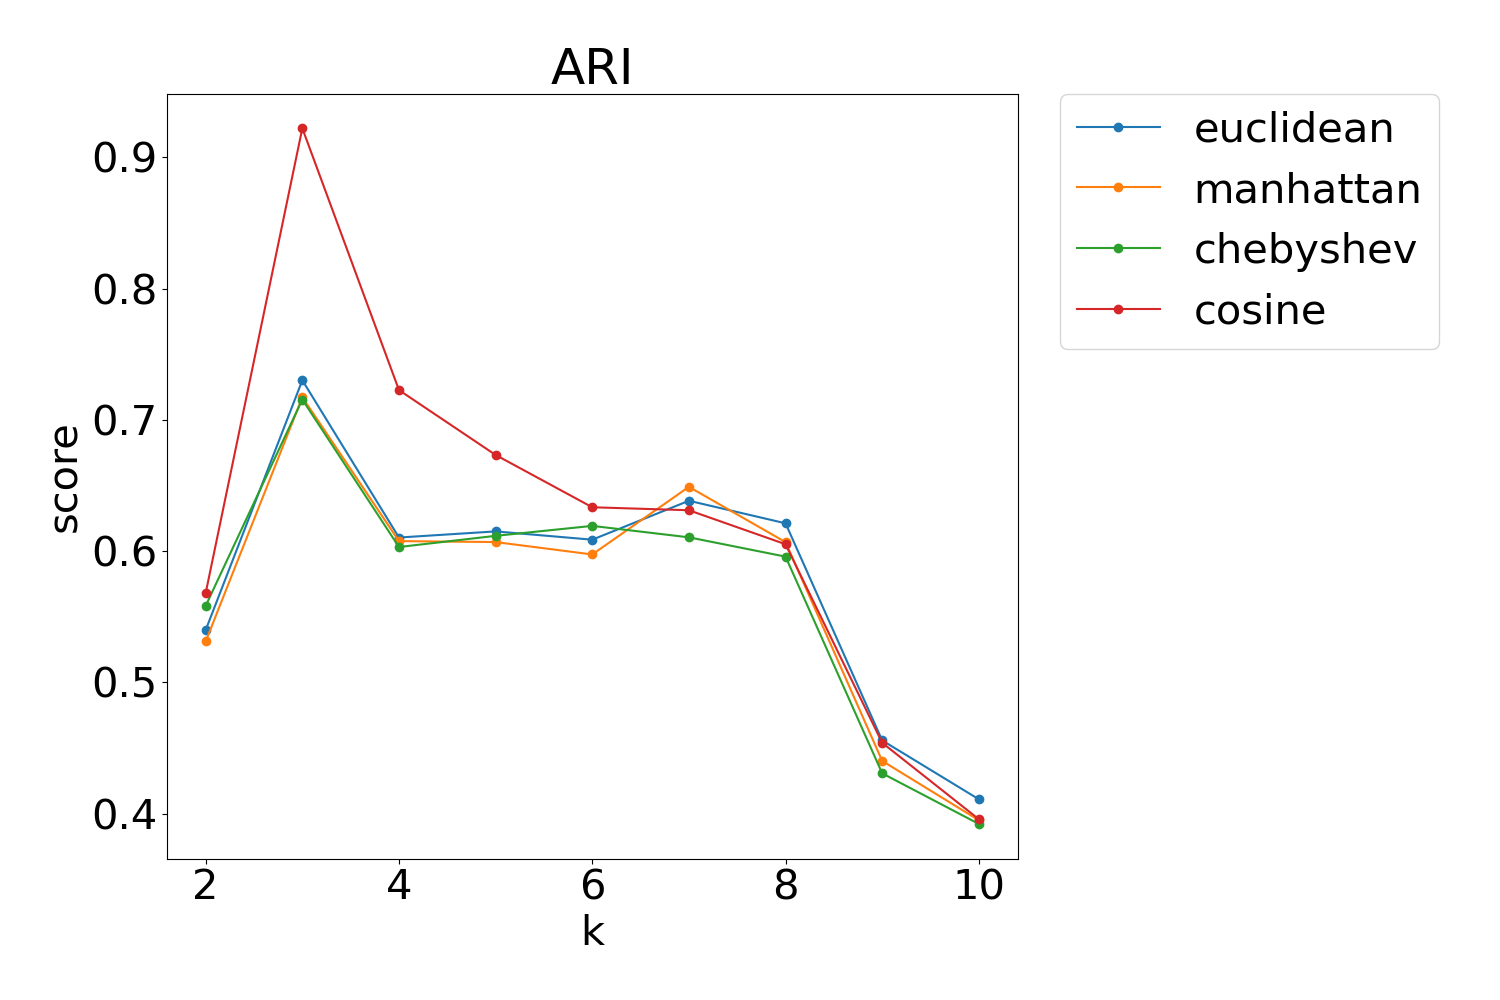
\includegraphics[width=0.45\textwidth]{../plots/iris/kmeans/ARI/k_1to10.png} }}%
	\qquad
	\subfloat[AMI ]{{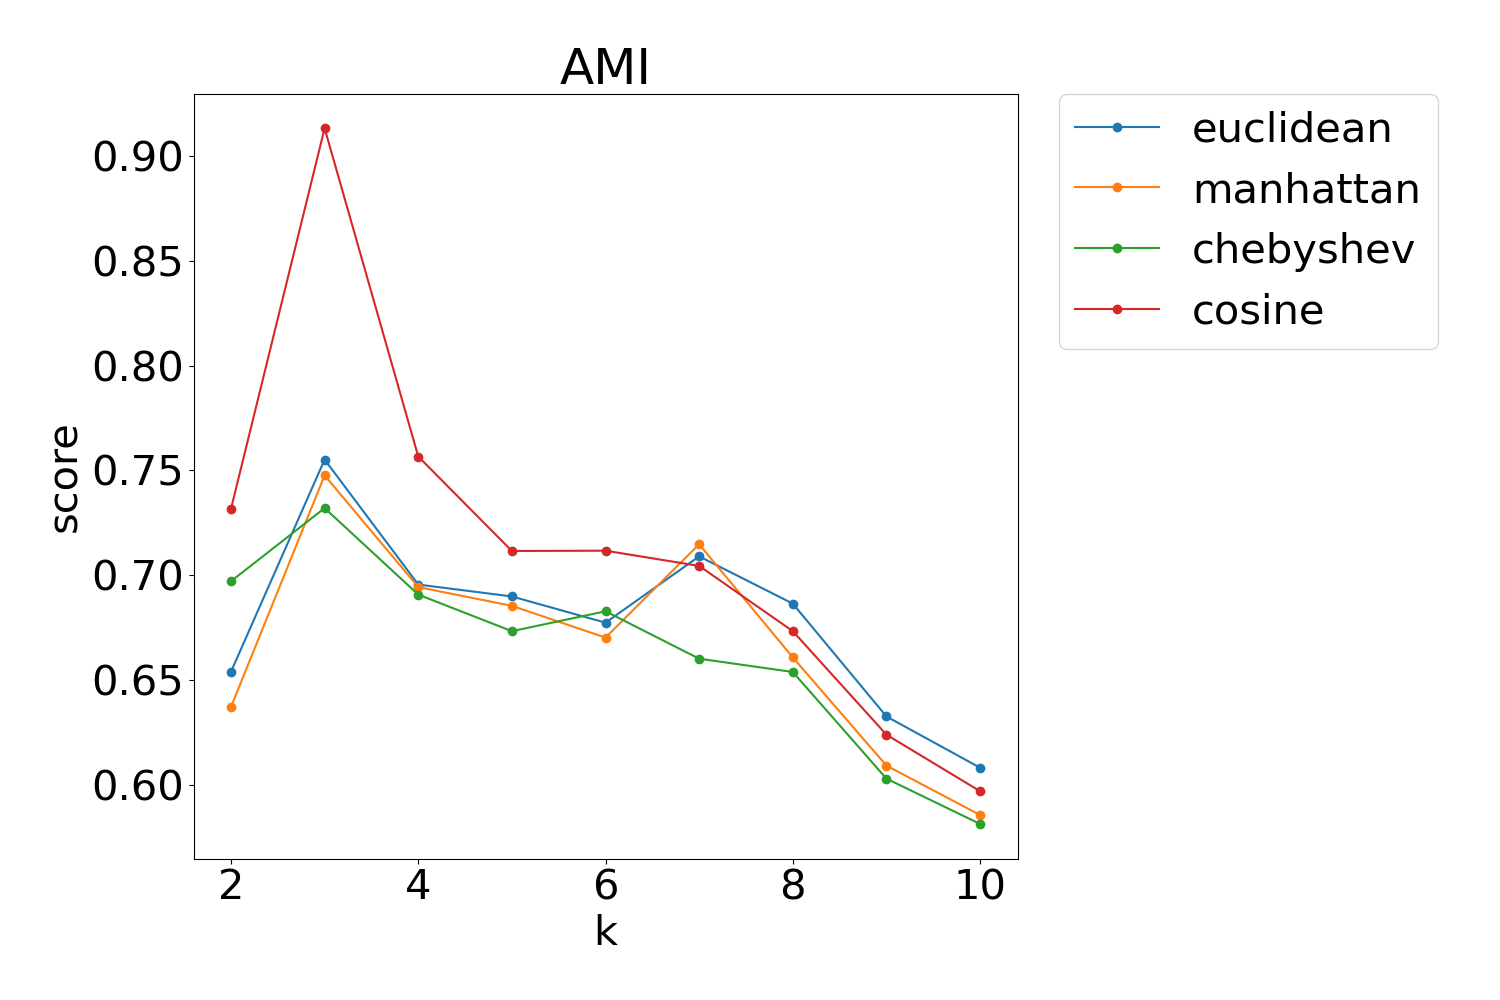
\includegraphics[width=0.45\textwidth]{../plots/iris/kmeans/AMI/k_1to10.png} }}%
	\qquad
	\subfloat[Completeness Score ]{{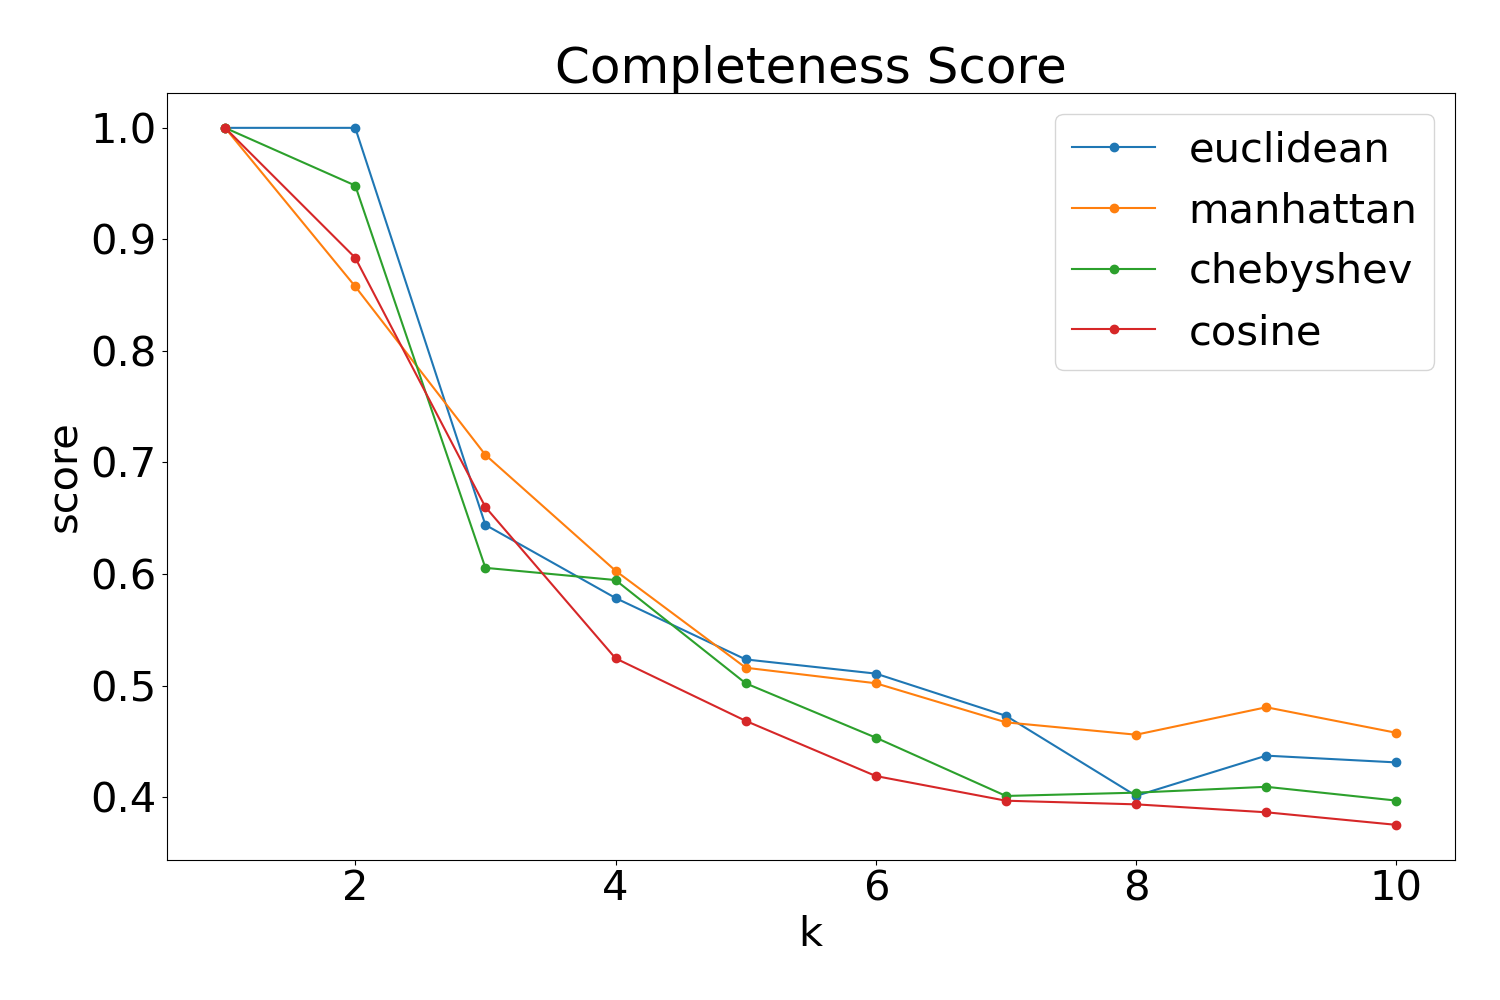
\includegraphics[width=0.45\textwidth]{../plots/iris/kmeans/Completeness Score/k_1to10.png} }}%
	\qquad
	\subfloat[Homogeneity Score ]{{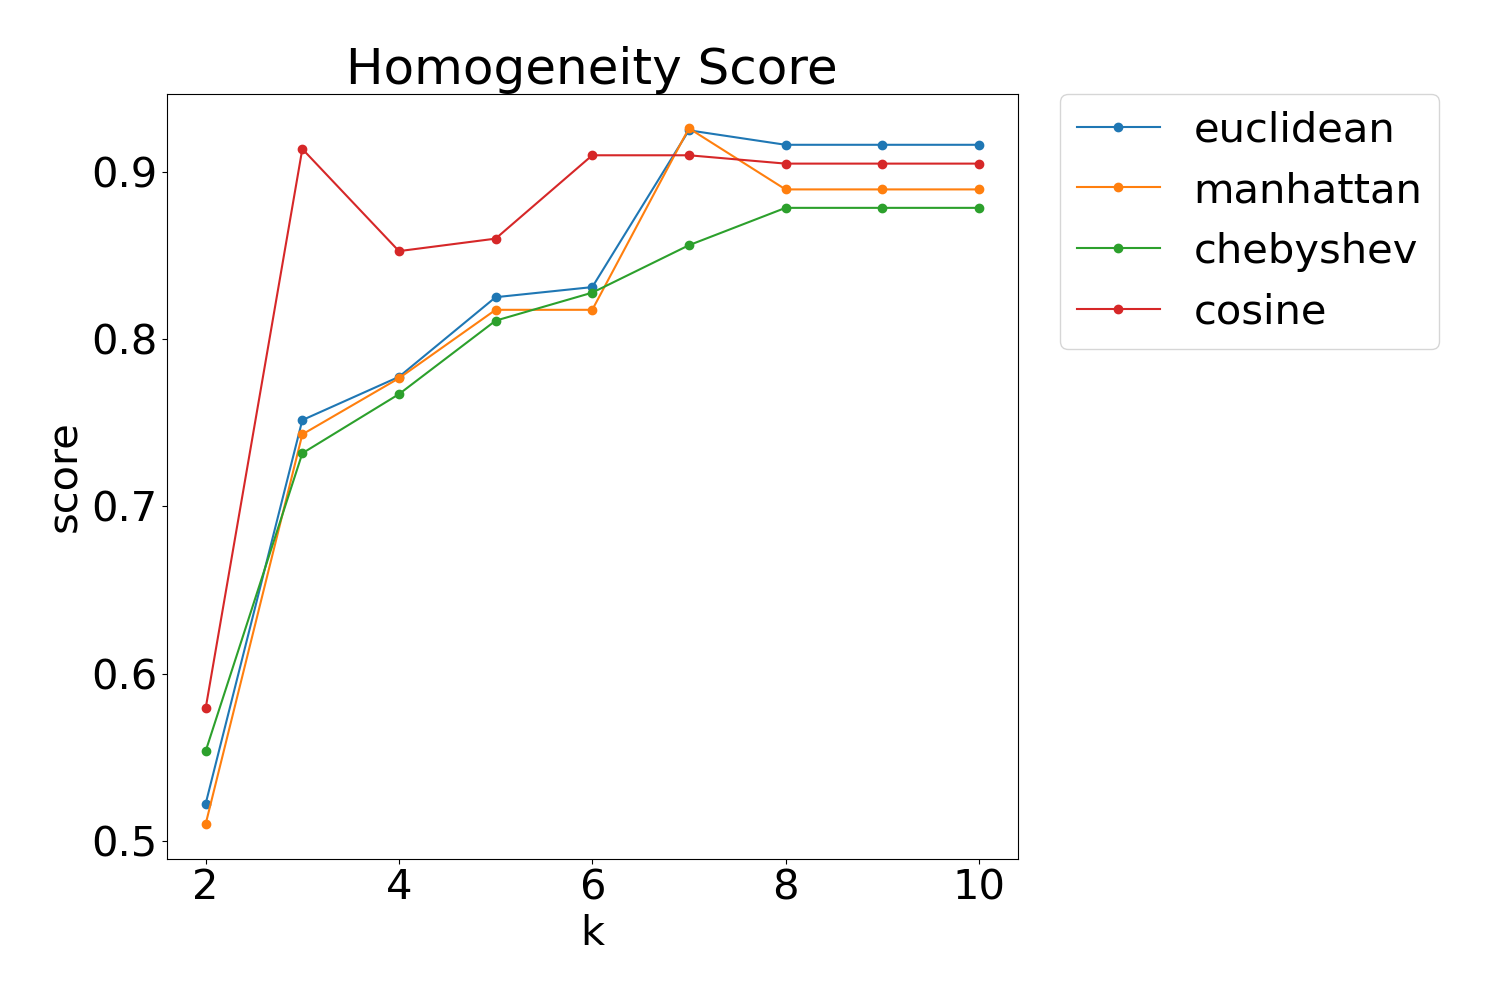
\includegraphics[width=0.45\textwidth]{../plots/iris/kmeans/Homogeneity Score/k_1to10.png} }}%
	\qquad
	\subfloat[Silhouette Score ]{{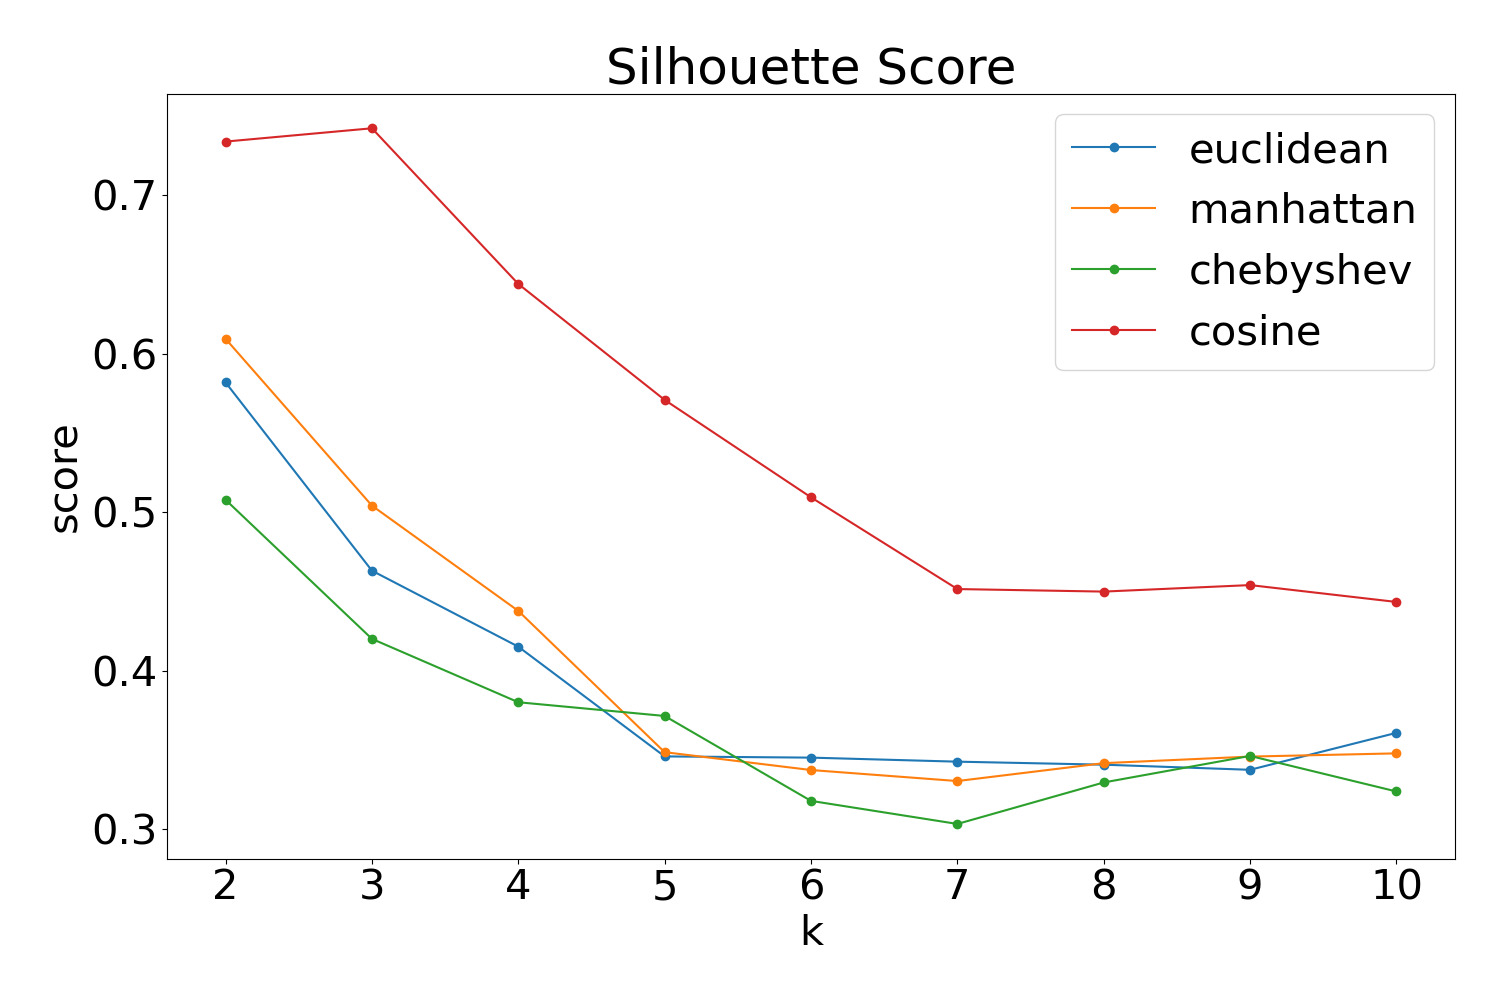
\includegraphics[width=1\textwidth]{../plots/iris/kmeans/Silhouette Score/k_1to10.png} }}%
	
	\caption{Comparison of clustering scores for K-Means-clustering on Iris dataset}%
	\label{fig:kmeans_iris}
\end{figure}

\begin{figure}[H]
	\centering
	\subfloat[ARI ]{{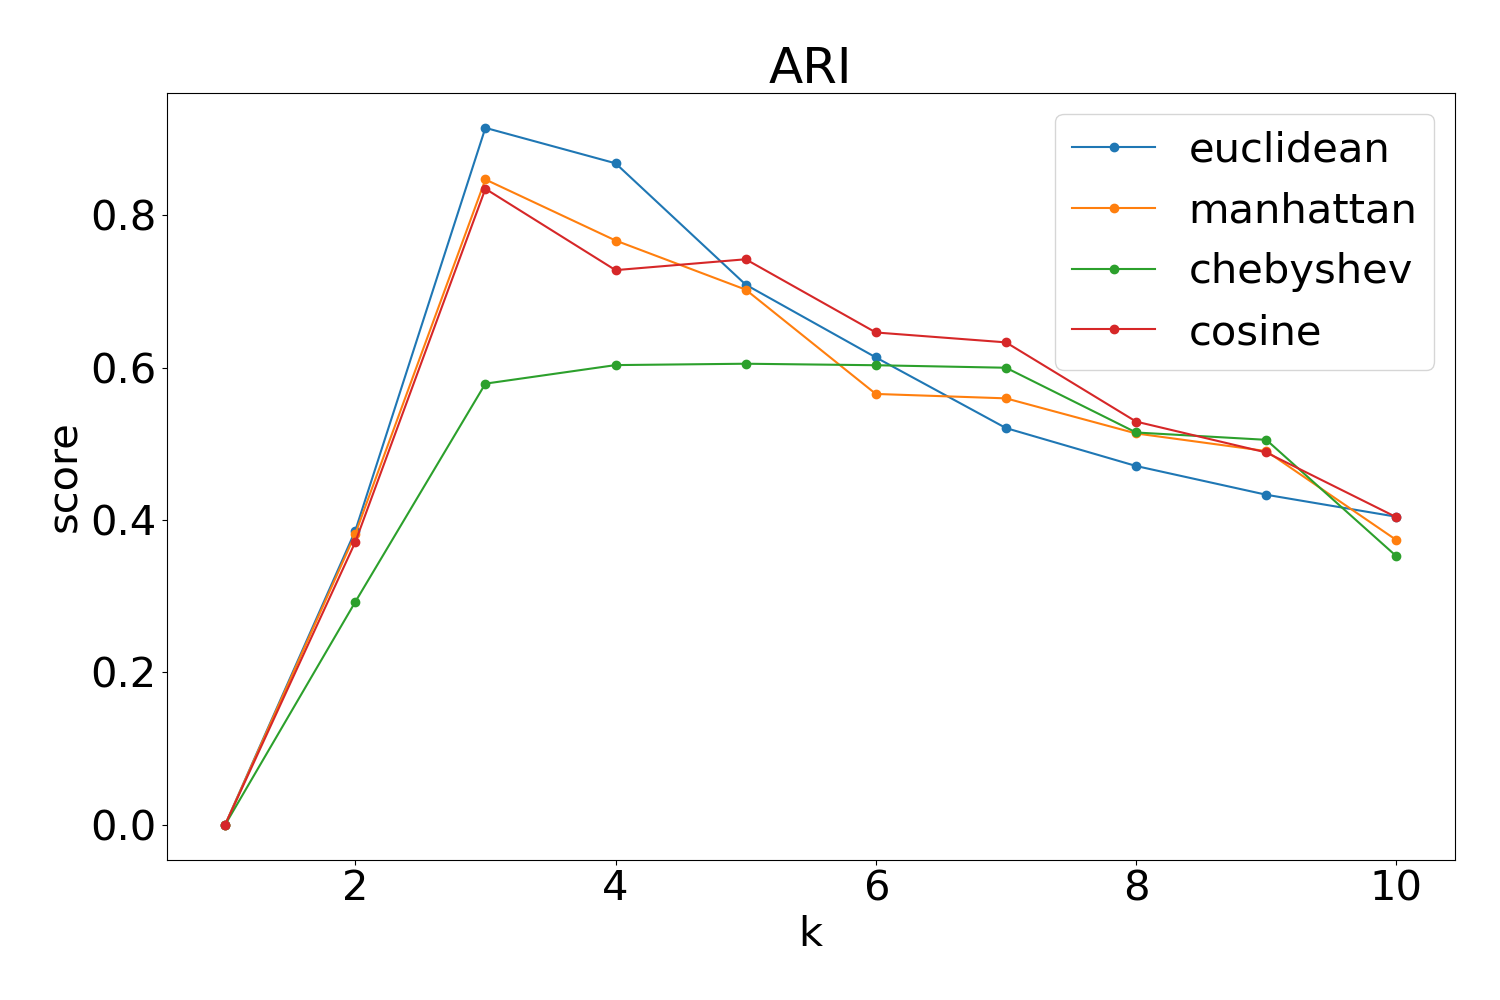
\includegraphics[width=0.45\textwidth]{../plots/wine/kmeans/ARI/k_1to10.png} }}%
	\qquad
	\subfloat[AMI ]{{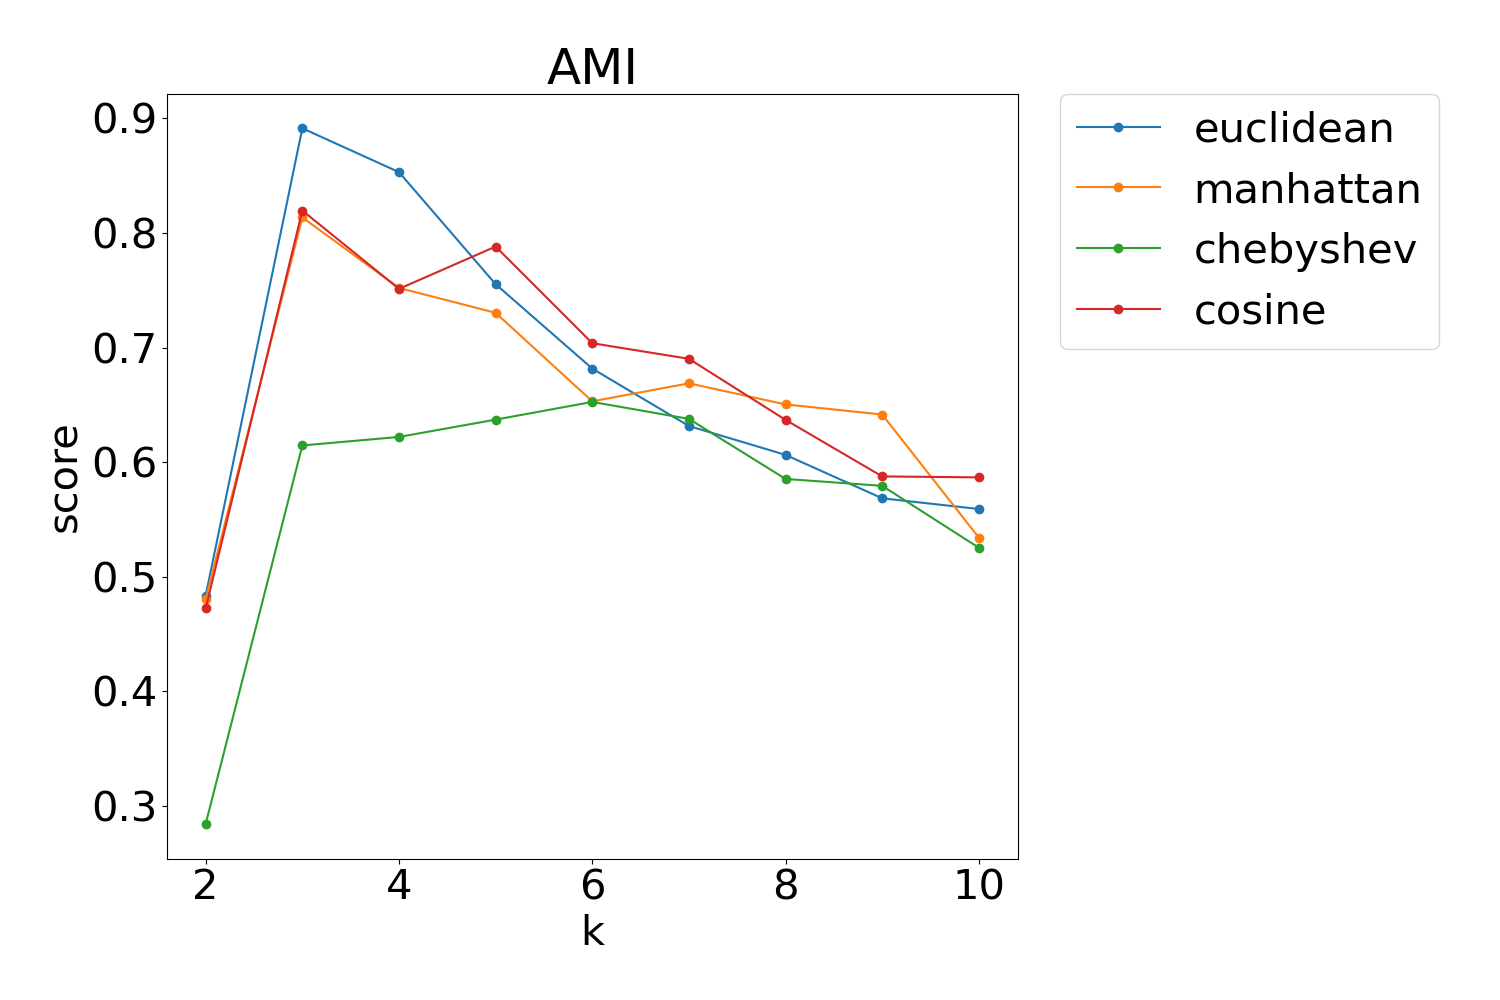
\includegraphics[width=0.45\textwidth]{../plots/wine/kmeans/AMI/k_1to10.png} }}%
	\qquad
	\subfloat[Completeness Score ]{{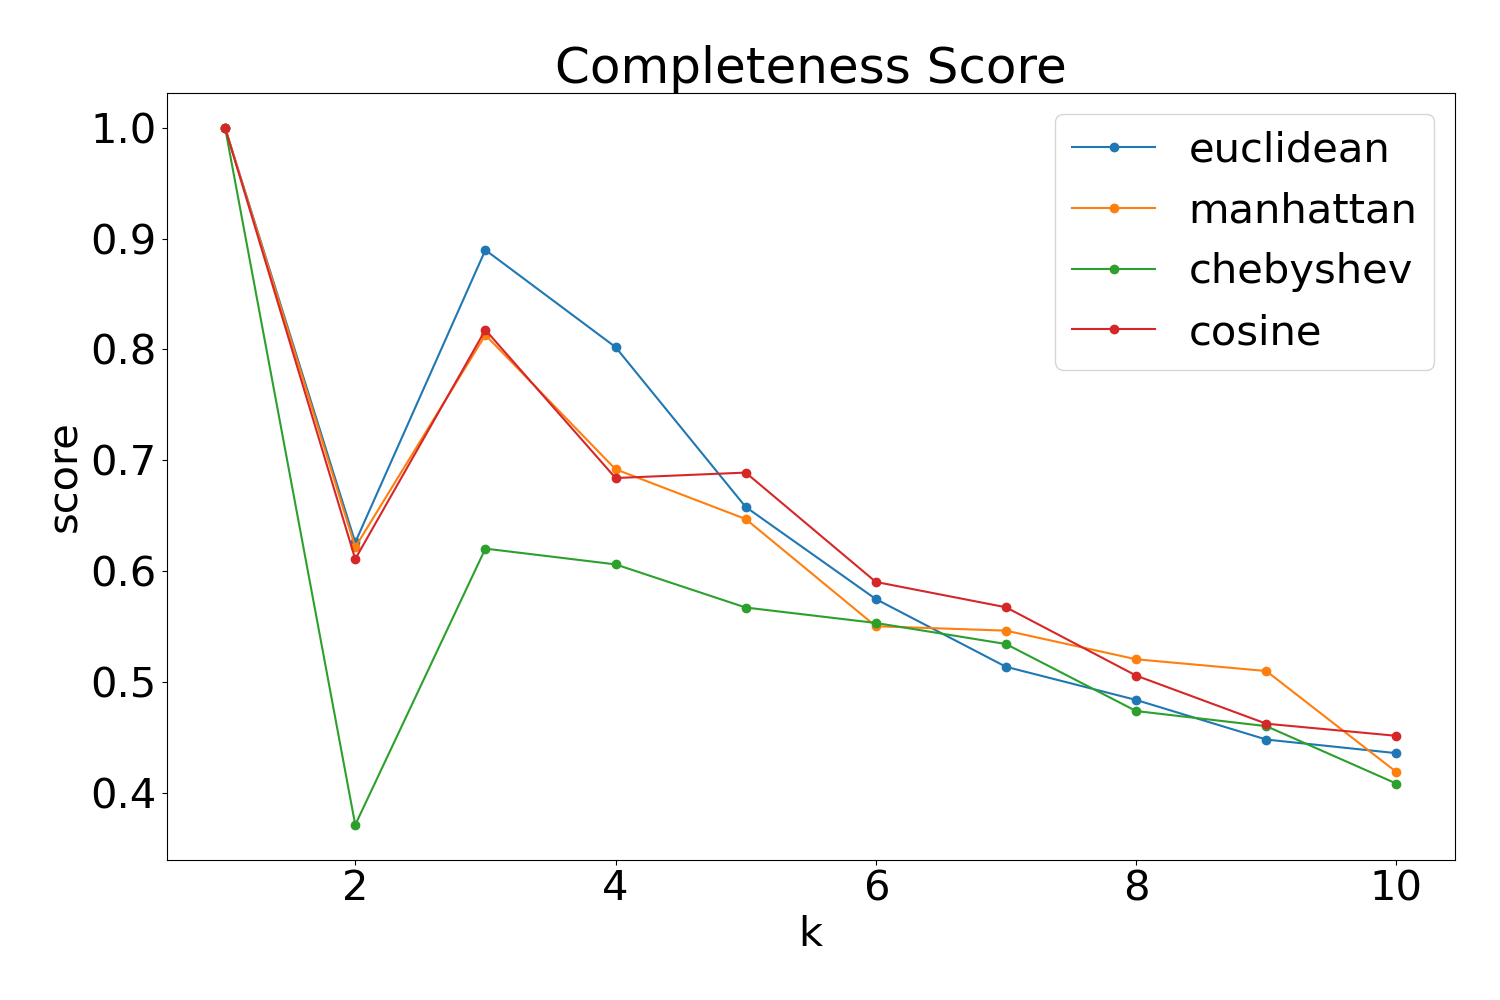
\includegraphics[width=0.45\textwidth]{../plots/wine/kmeans/Completeness Score/k_1to10.png} }}%
	\qquad
	\subfloat[Homogeneity Score ]{{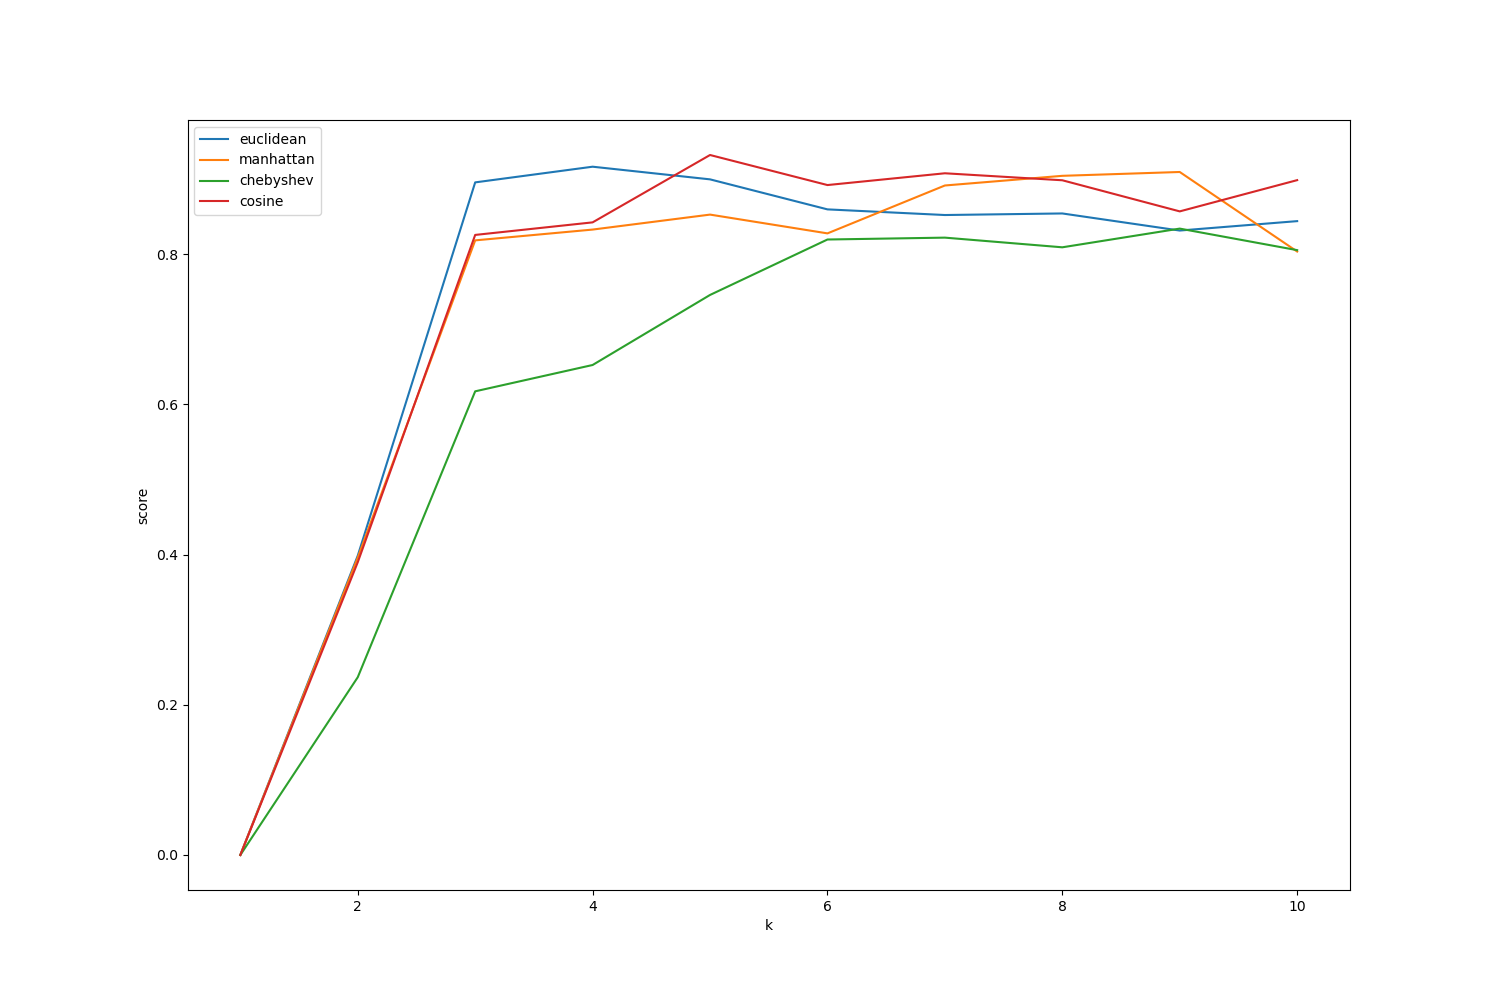
\includegraphics[width=0.45\textwidth]{../plots/wine/kmeans/Homogeneity Score/k_1to10.png} }}%
	\qquad
	\subfloat[Silhouette Score ]{{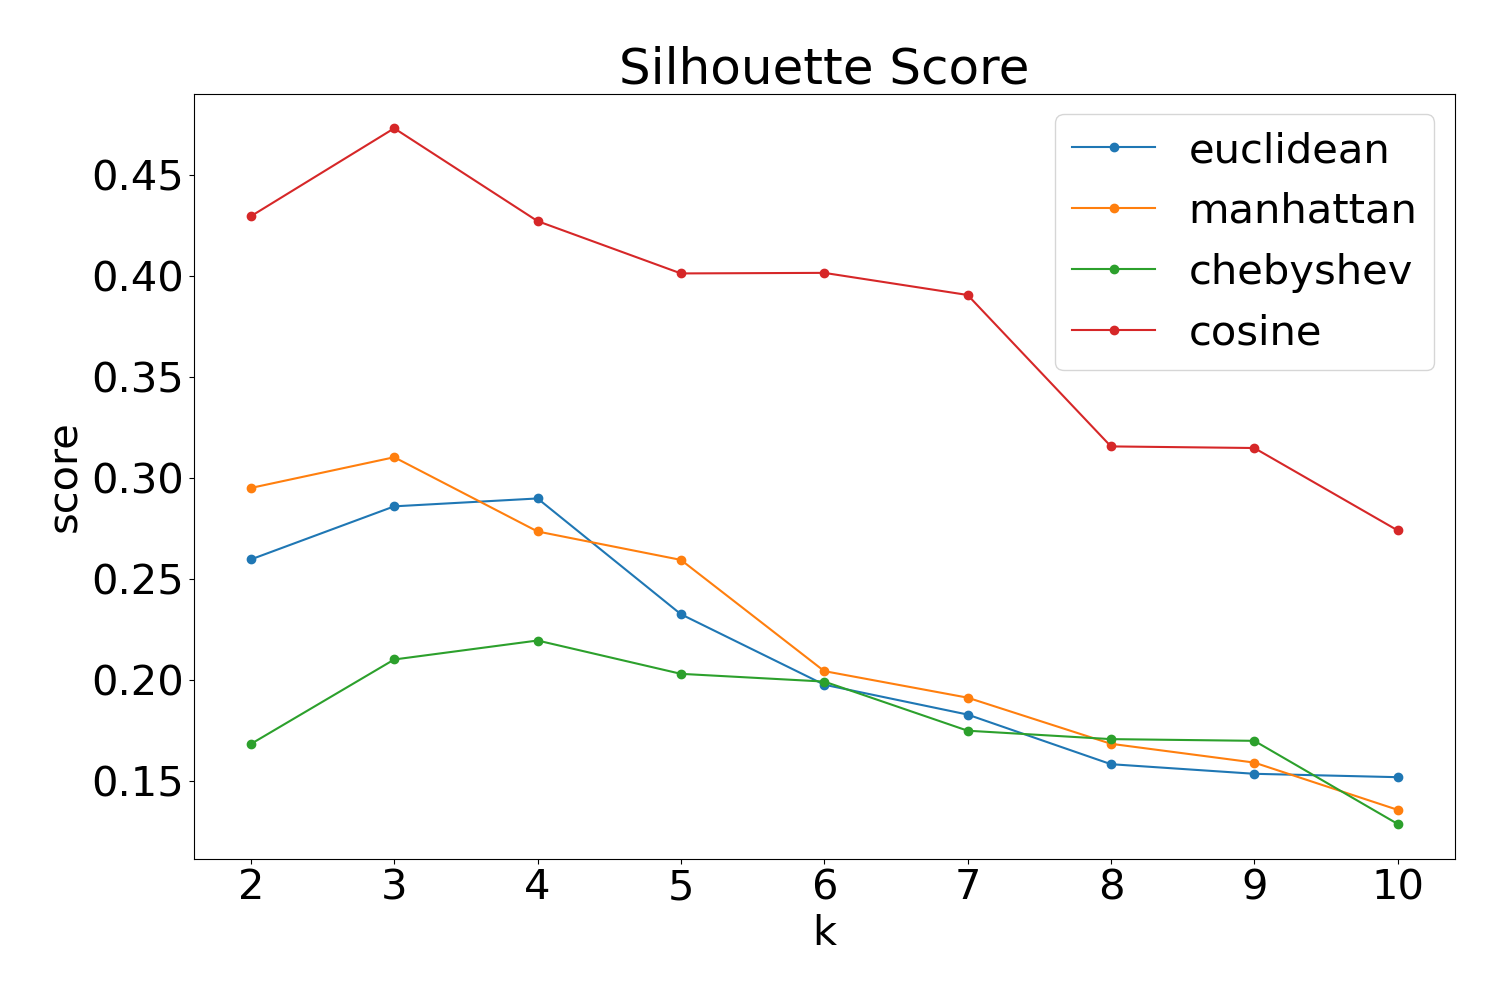
\includegraphics[width=1\textwidth]{../plots/wine/kmeans/Silhouette Score/k_1to10.png} }}%
	
	\caption{Comparison of clustering scores for K-Means-clustering on Wine dataset}%
	\label{fig:kmeans_wine}
\end{figure}

\begin{figure}[H]
	\centering
	\subfloat[Silhouette Score ]{{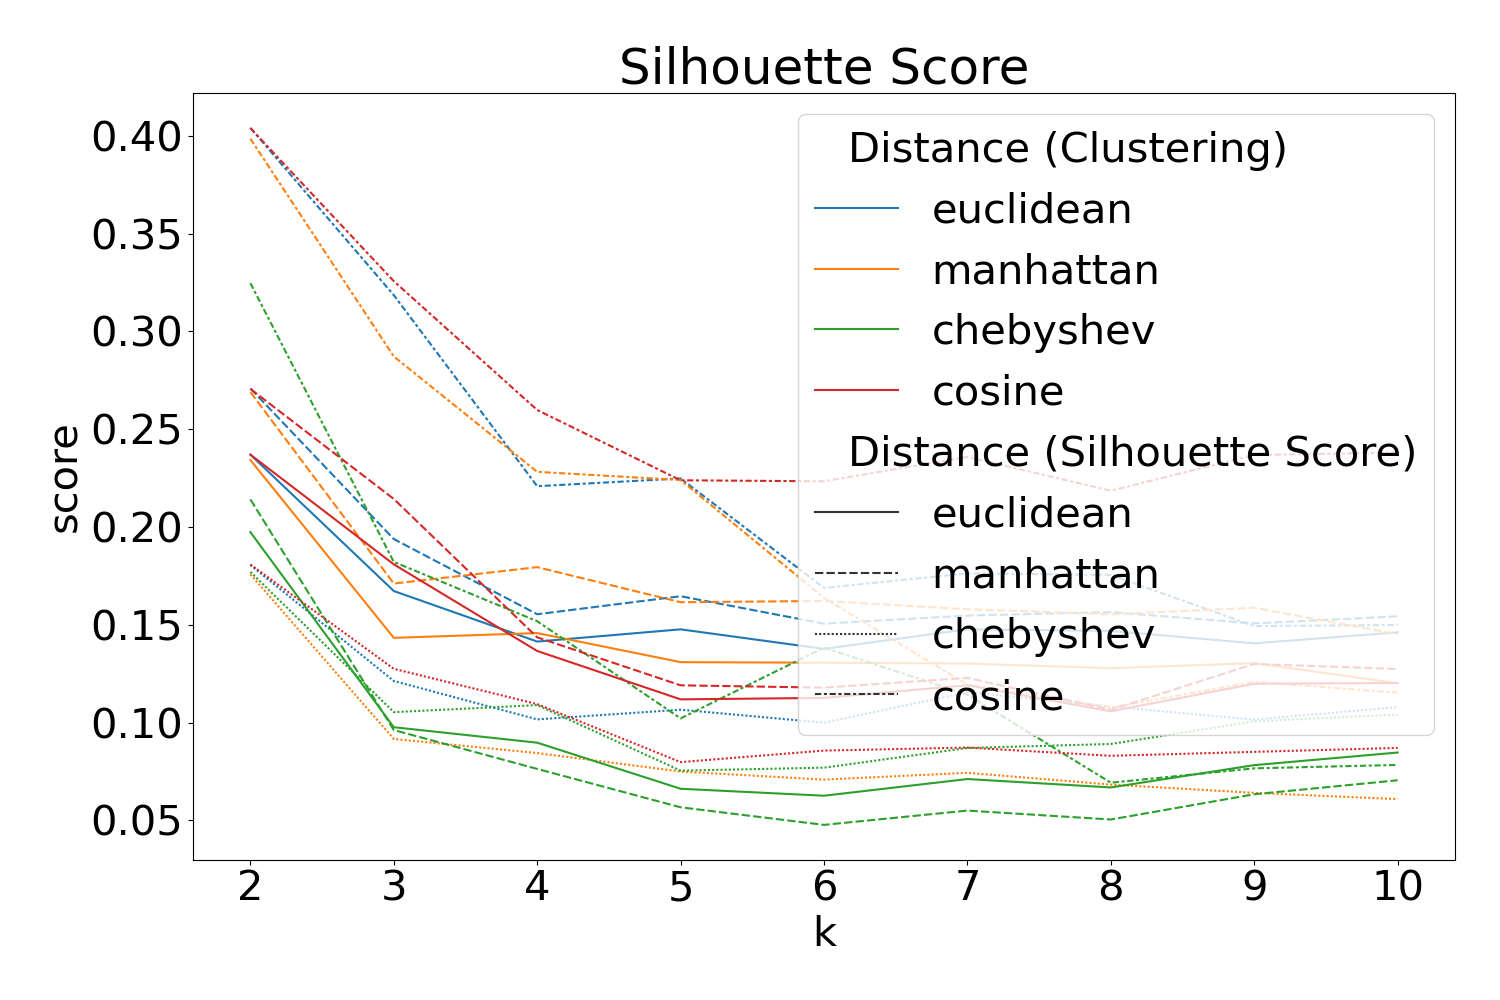
\includegraphics[width=1\textwidth]{../plots/diabetes/kmeans/Silhouette Score/k_1to10.png} }}%
	
	\caption{Comparison of clustering scores for K-Means-clustering on Diabetes dataset}%
	\label{fig:kmeans_diabetes}
\end{figure}

\begin{figure}[H]
	\centering
	\subfloat[ARI ]{{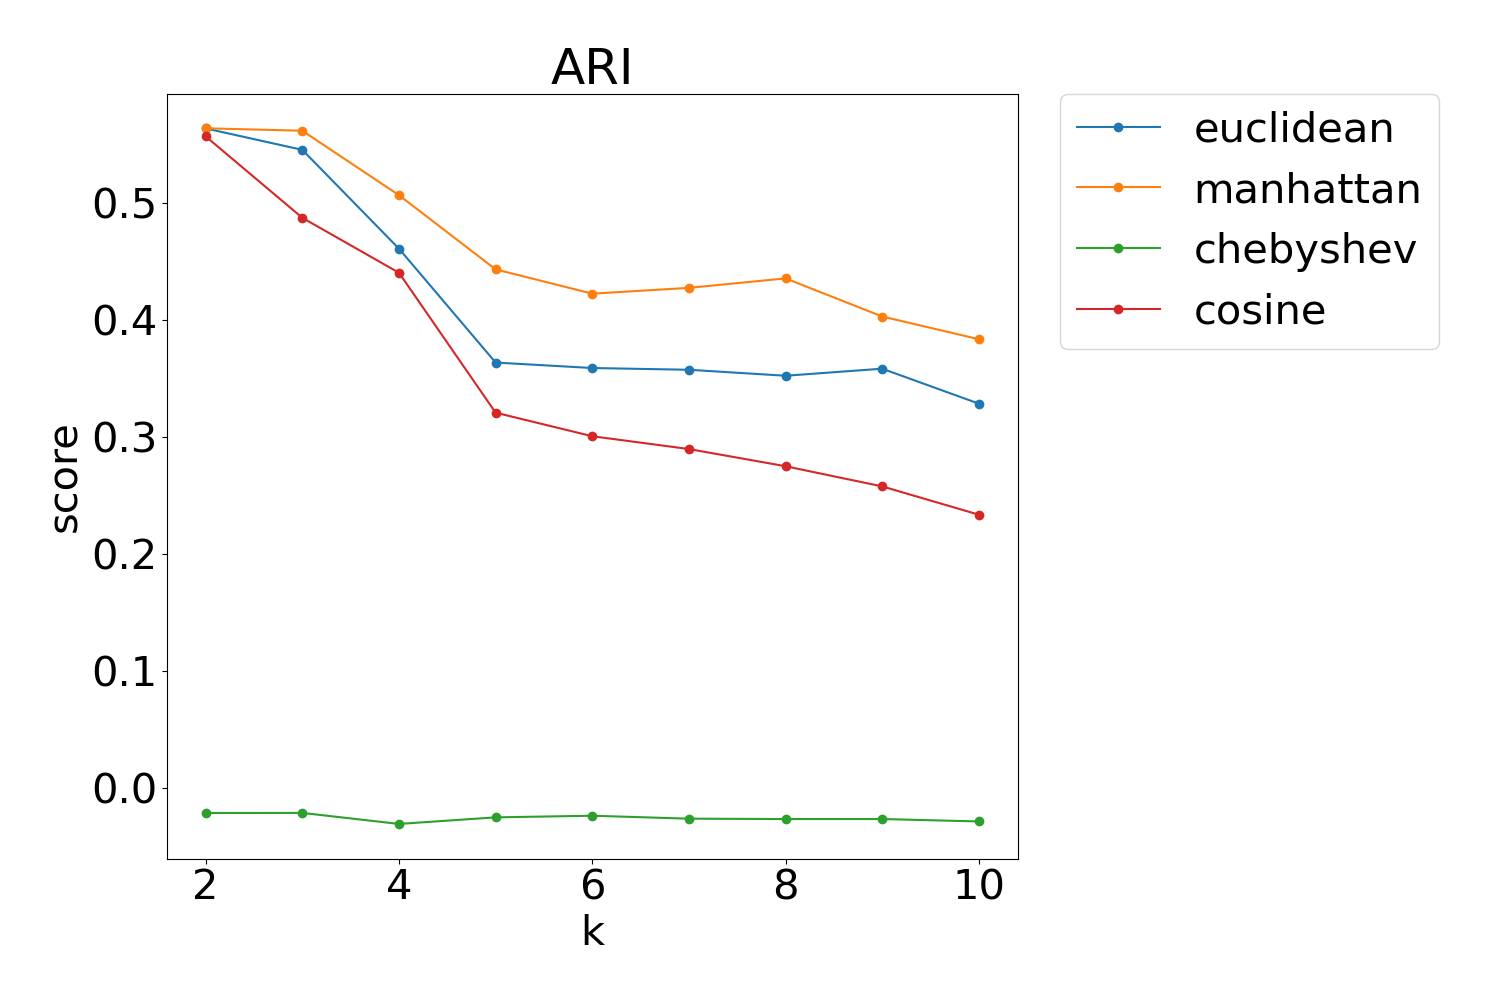
\includegraphics[width=0.45\textwidth]{../plots/housevotes/kmeans/ARI/k_1to10.png} }}%
	\qquad
	\subfloat[AMI ]{{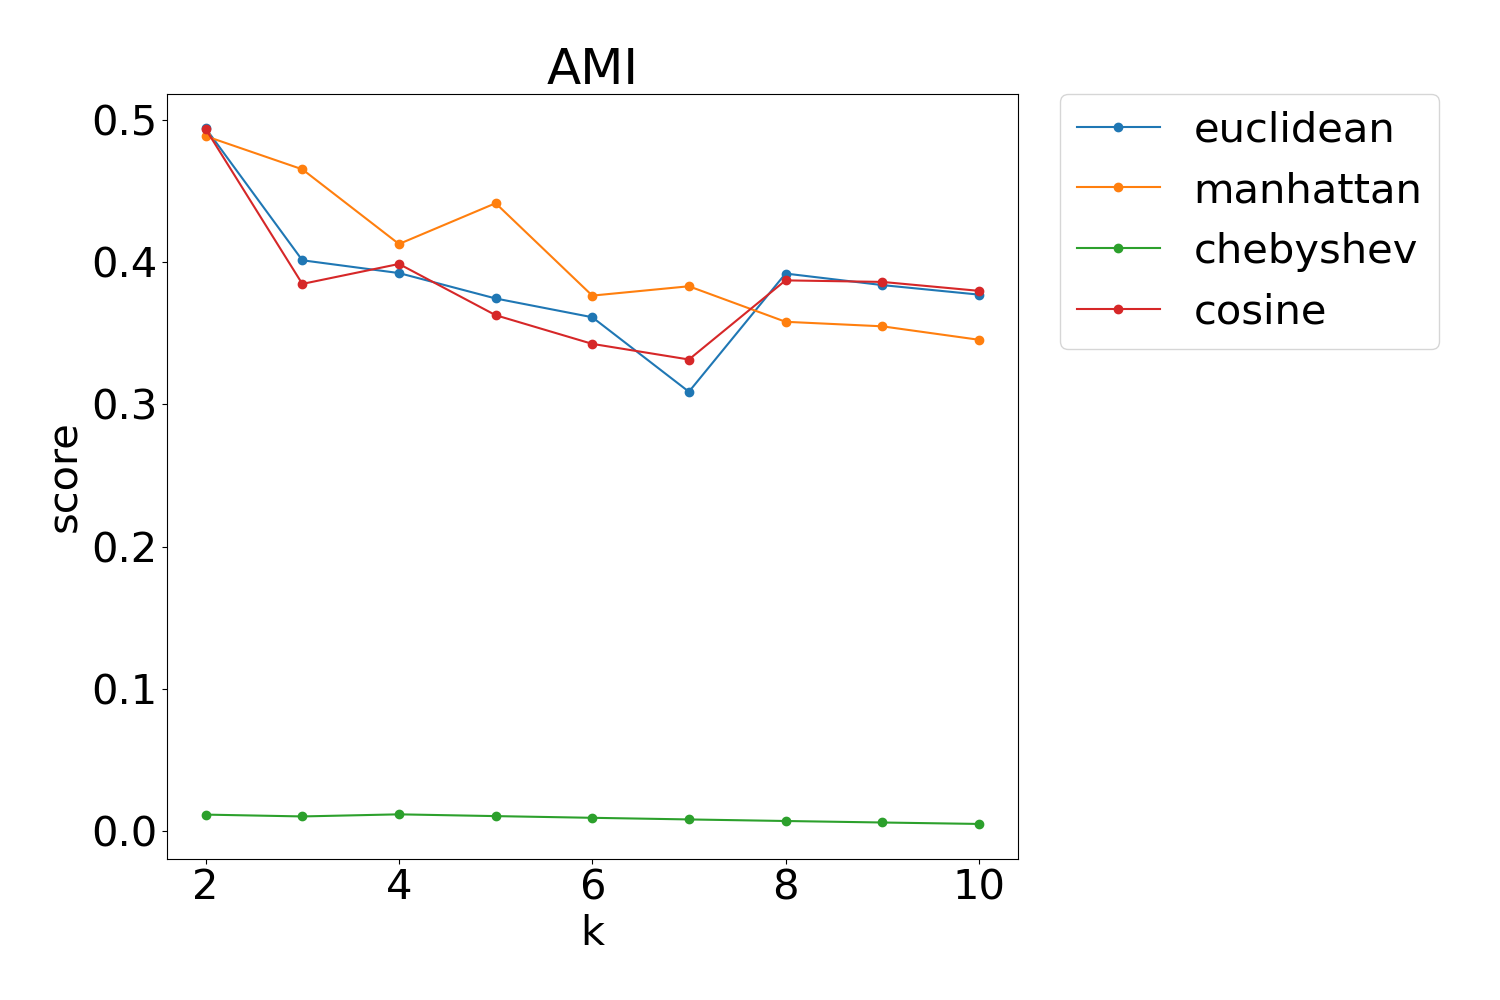
\includegraphics[width=0.45\textwidth]{../plots/housevotes/kmeans/AMI/k_1to10.png} }}%
	\qquad
	\subfloat[Completeness Score ]{{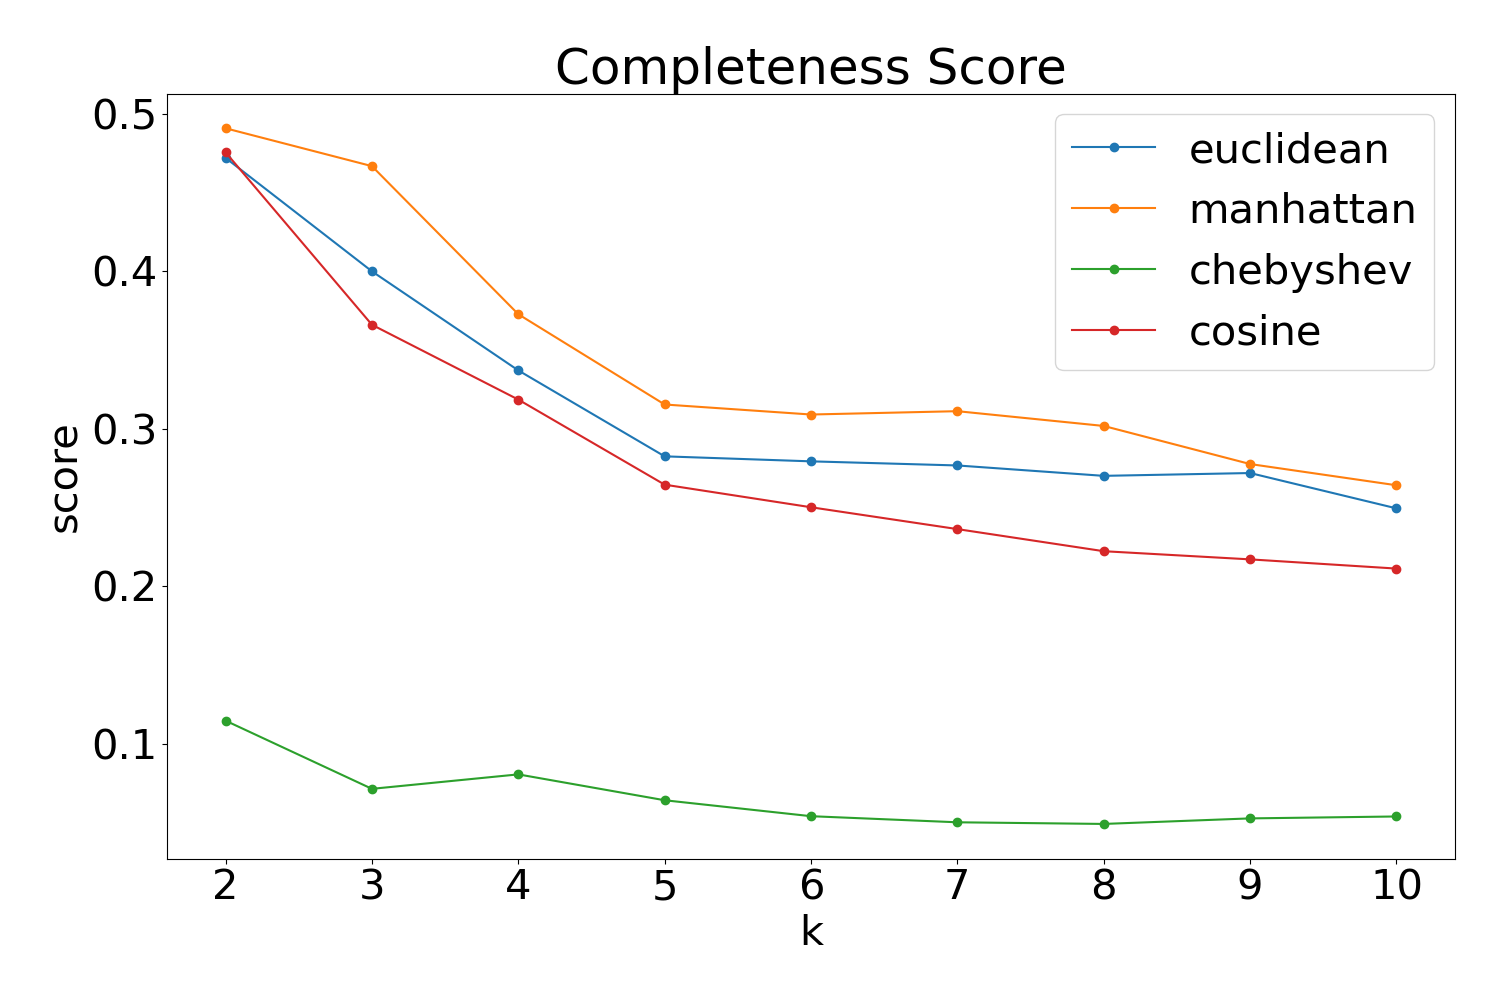
\includegraphics[width=0.45\textwidth]{../plots/housevotes/kmeans/Completeness Score/k_1to10.png} }}%
	\qquad
	\subfloat[Homogeneity Score ]{{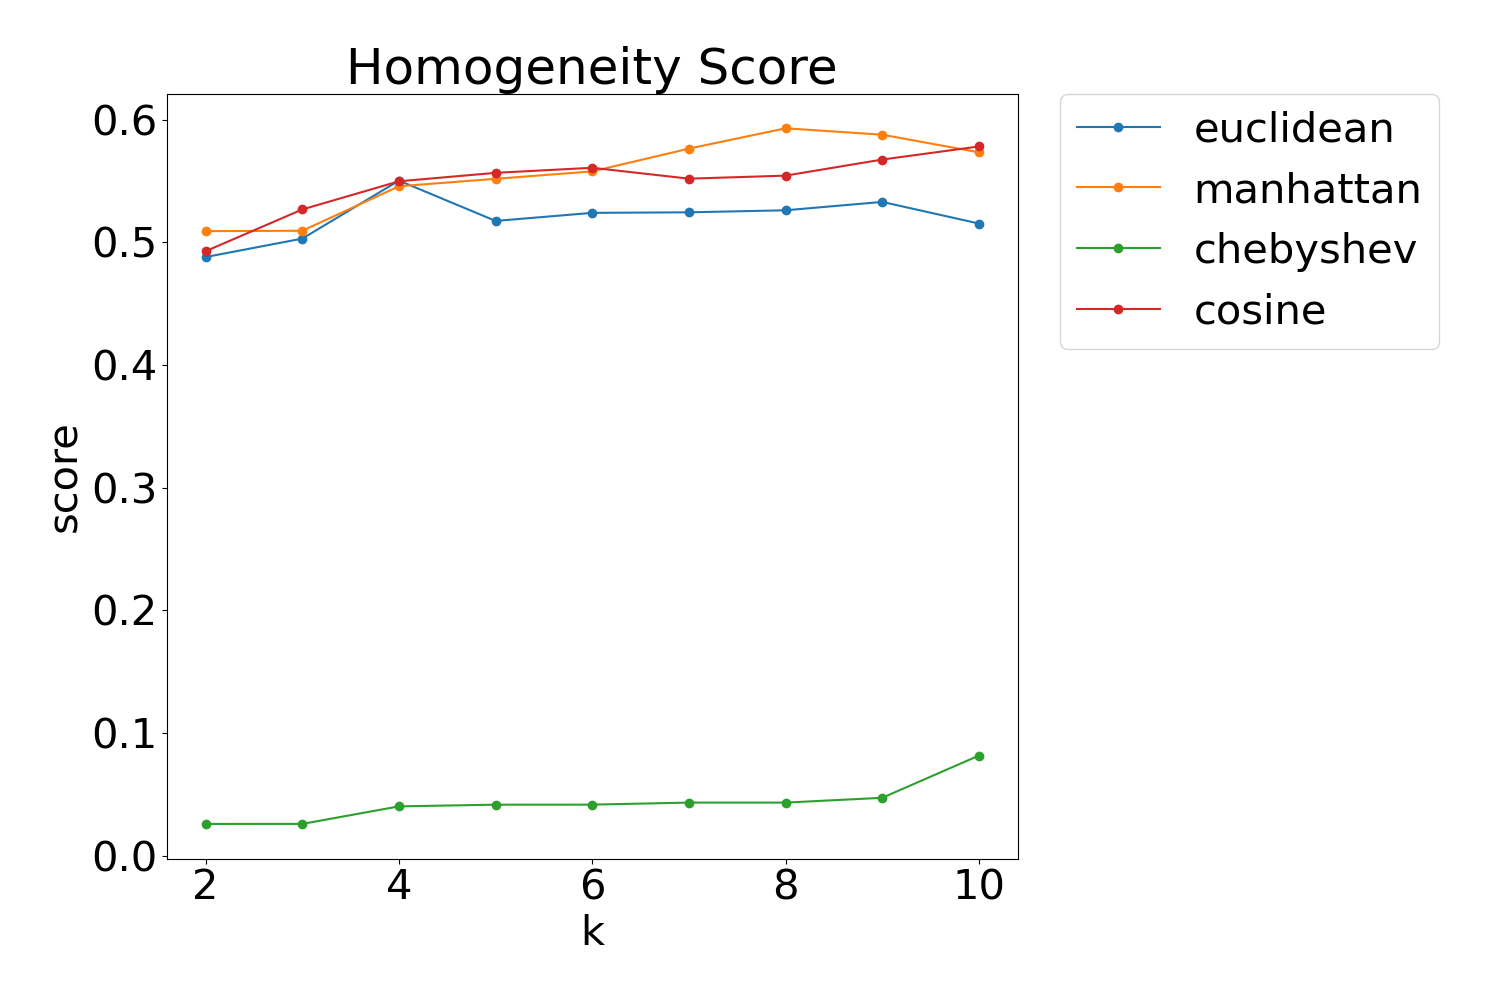
\includegraphics[width=0.45\textwidth]{../plots/housevotes/kmeans/Homogeneity Score/k_1to10.png} }}%
	\qquad
	\subfloat[Silhouette Score ]{{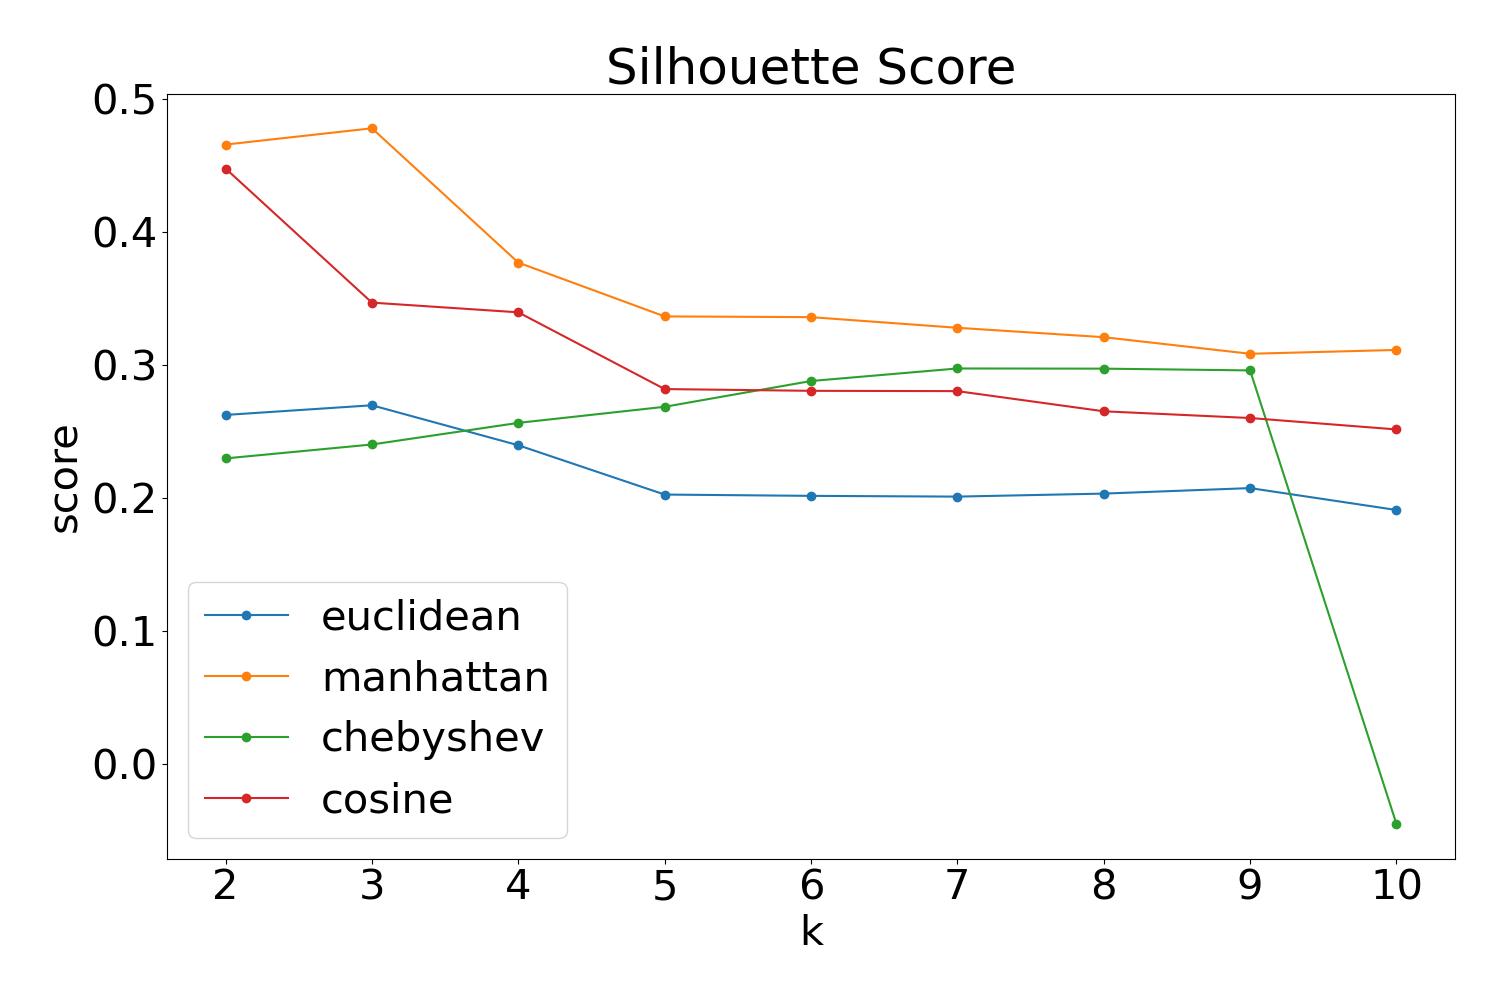
\includegraphics[width=1\textwidth]{../plots/housevotes/kmeans/Silhouette Score/k_1to10.png} }}%
	
	\caption{Comparison of clustering scores for K-Means-clustering on Housevotes dataset}%
	\label{fig:kmeans_housevotes}
\end{figure}

\begin{figure}[H]
	\centering
	\subfloat[ARI ]{{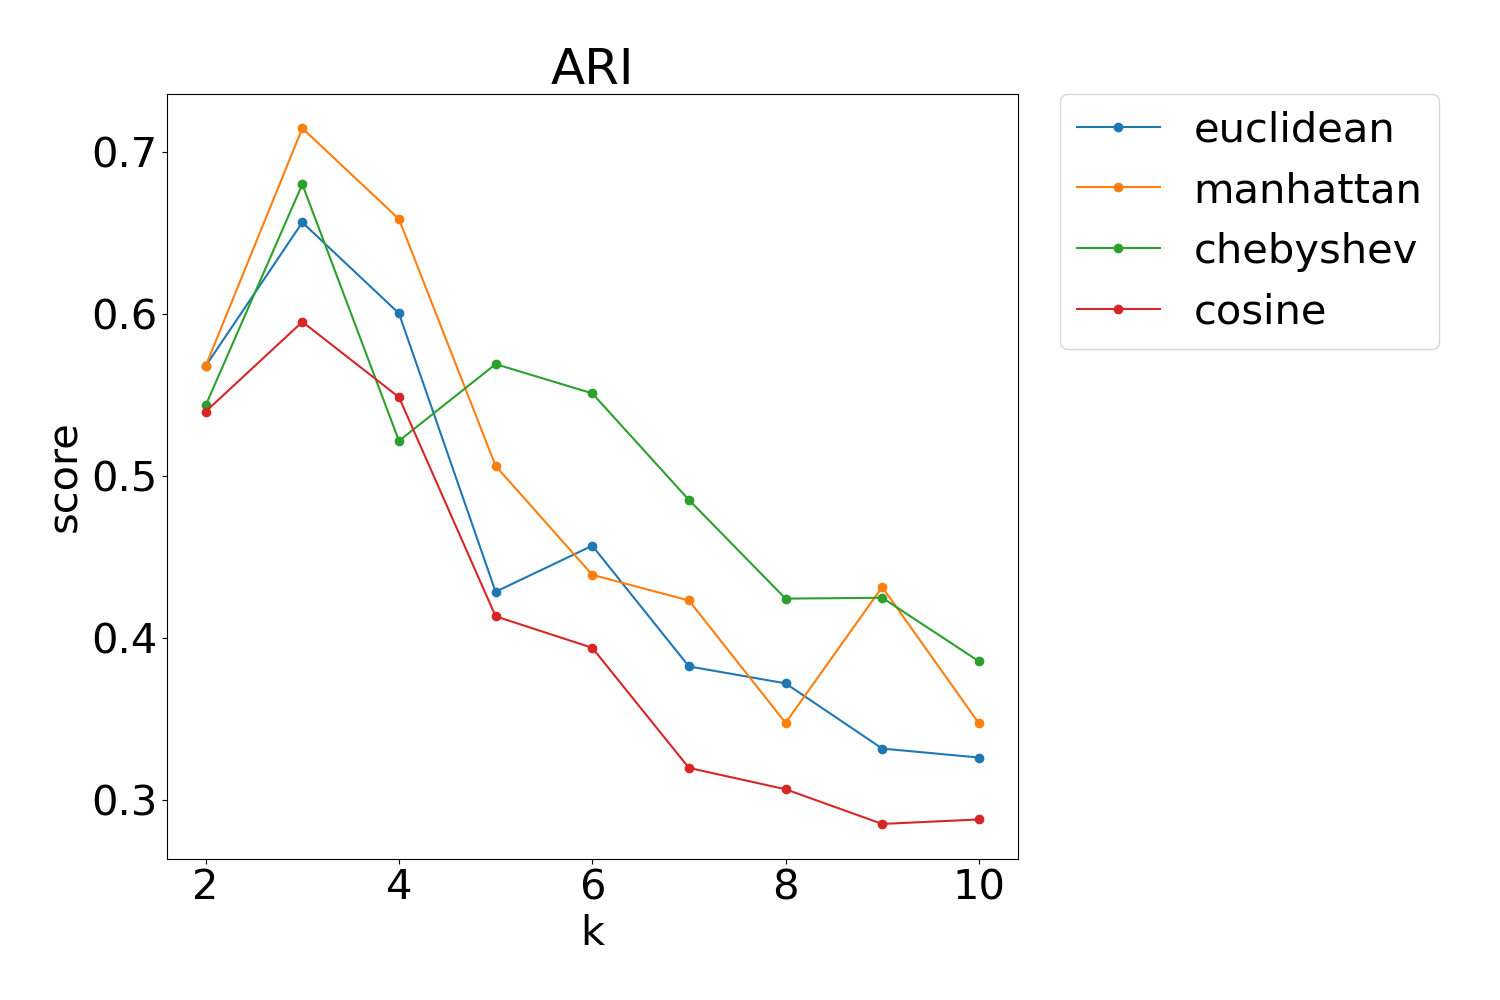
\includegraphics[width=0.45\textwidth]{../plots/iris/kmedians/ARI/k_1to10.png} }}%
	\qquad
	\subfloat[AMI ]{{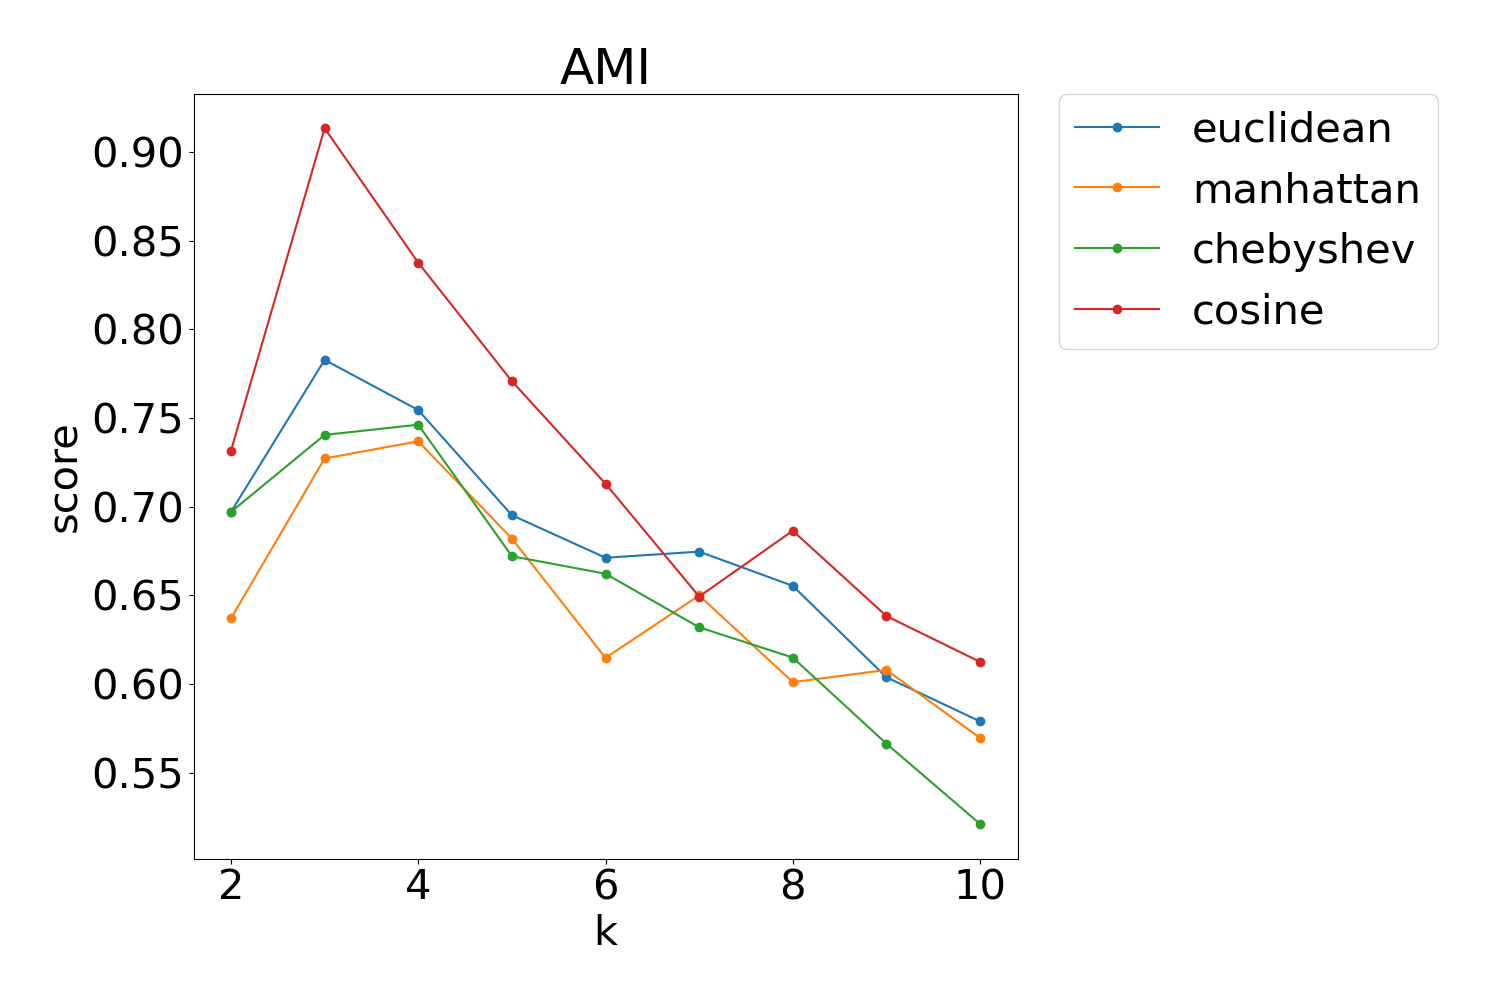
\includegraphics[width=0.45\textwidth]{../plots/iris/kmedians/AMI/k_1to10.png} }}%
	\qquad
	\subfloat[Completeness Score ]{{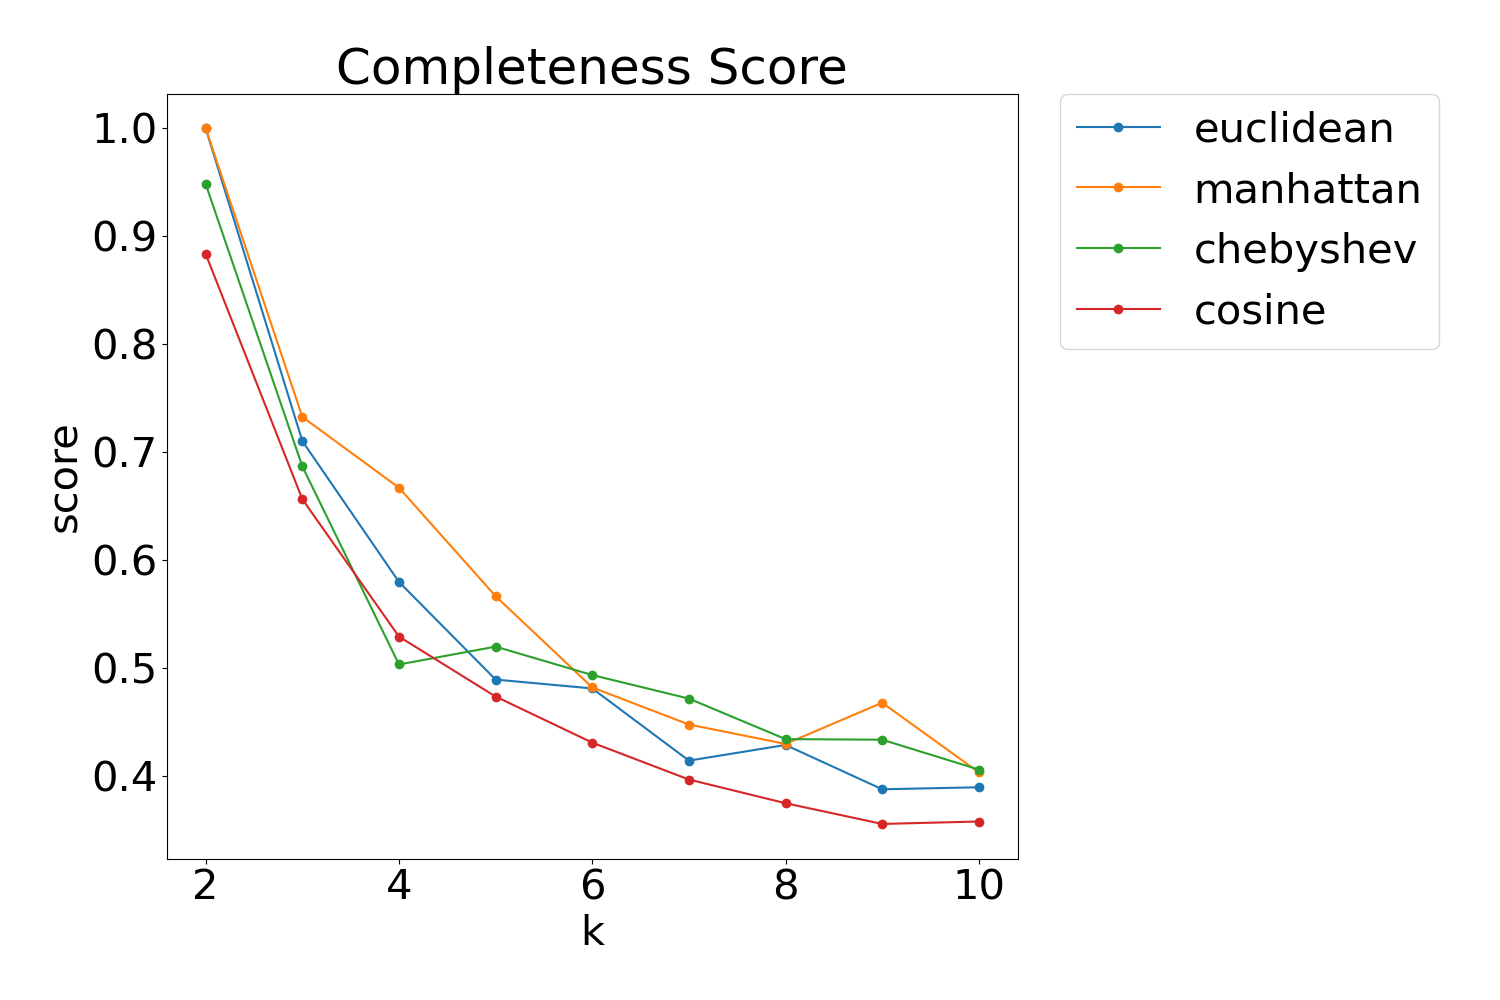
\includegraphics[width=0.45\textwidth]{../plots/iris/kmedians/Completeness Score/k_1to10.png} }}%
	\qquad
	\subfloat[Homogeneity Score ]{{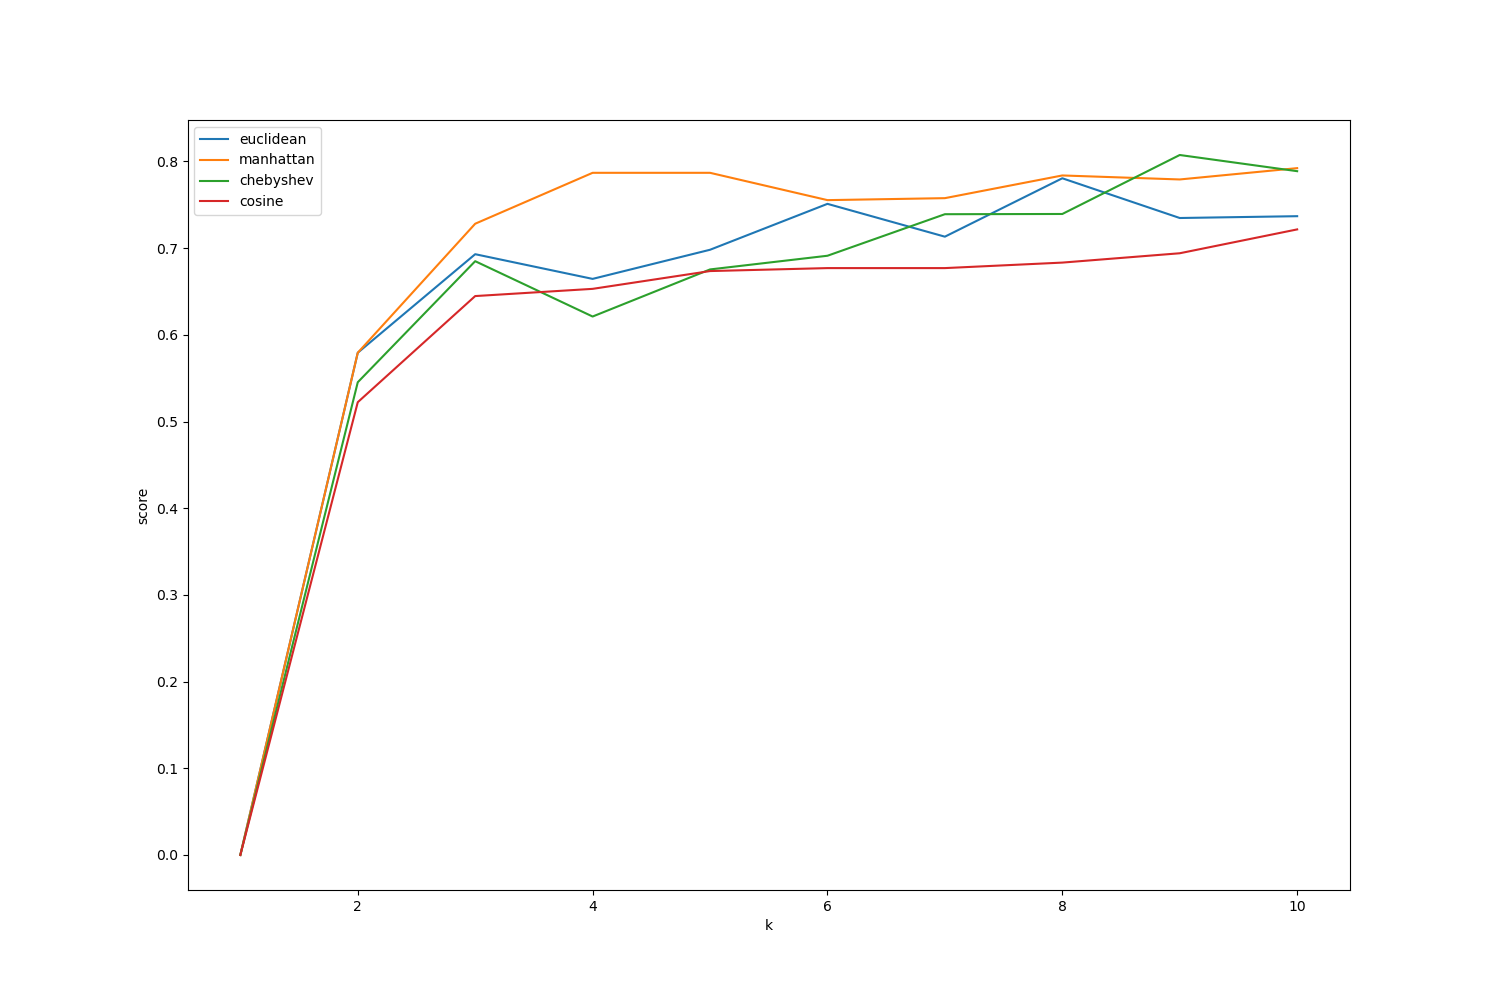
\includegraphics[width=0.45\textwidth]{../plots/iris/kmedians/Homogeneity Score/k_1to10.png} }}%
	\qquad
	\subfloat[Silhouette Score ]{{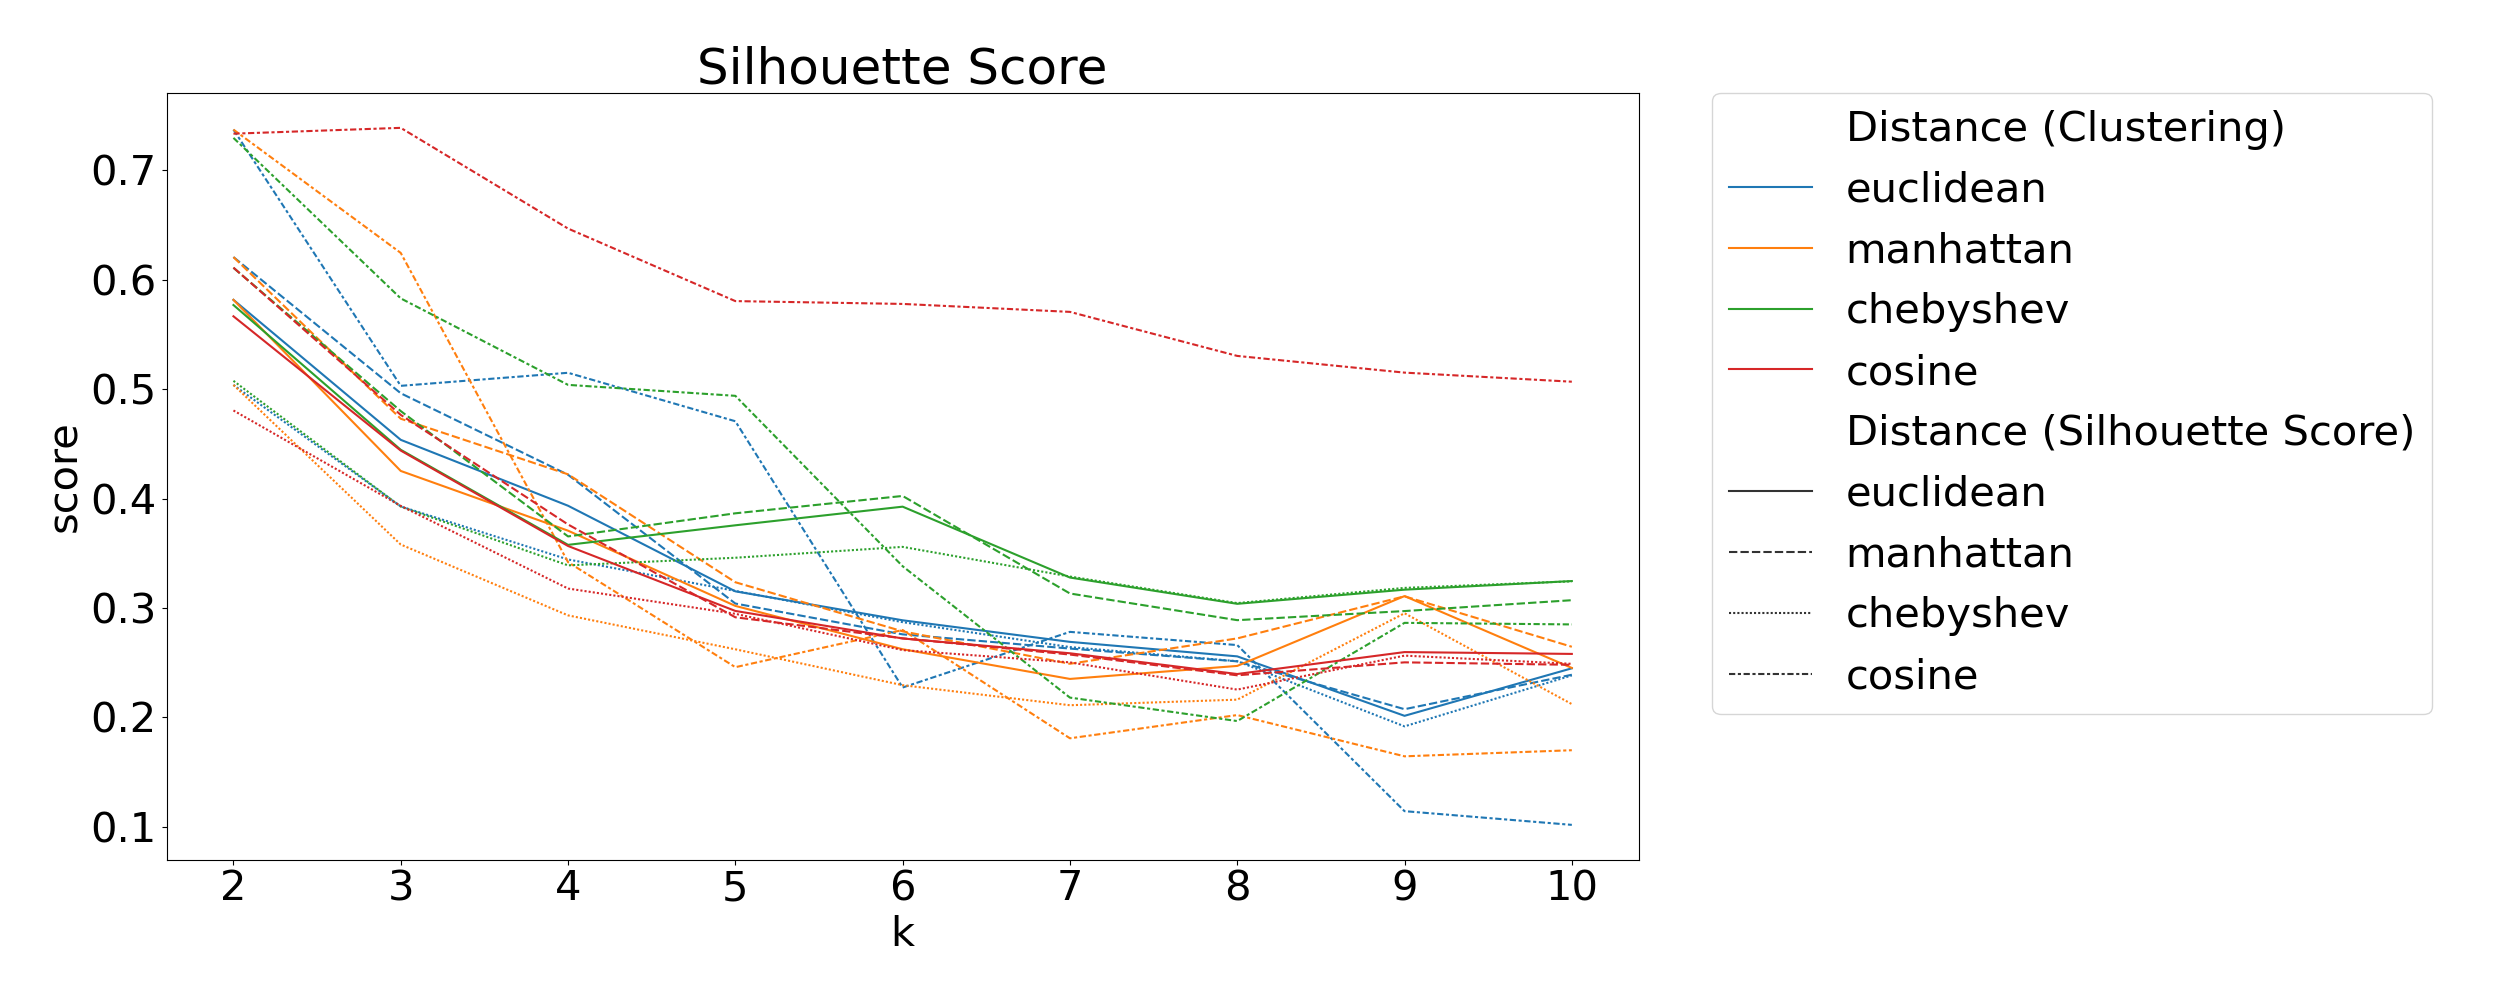
\includegraphics[width=1\textwidth]{../plots/iris/kmedians/Silhouette Score/k_1to10.png} }}%
	
	\caption{Comparison of clustering scores for K-Medians-clustering on Iris dataset}%
	\label{fig:kmedians_iris}
\end{figure}

\begin{figure}[H]
	\centering
	\subfloat[ARI ]{{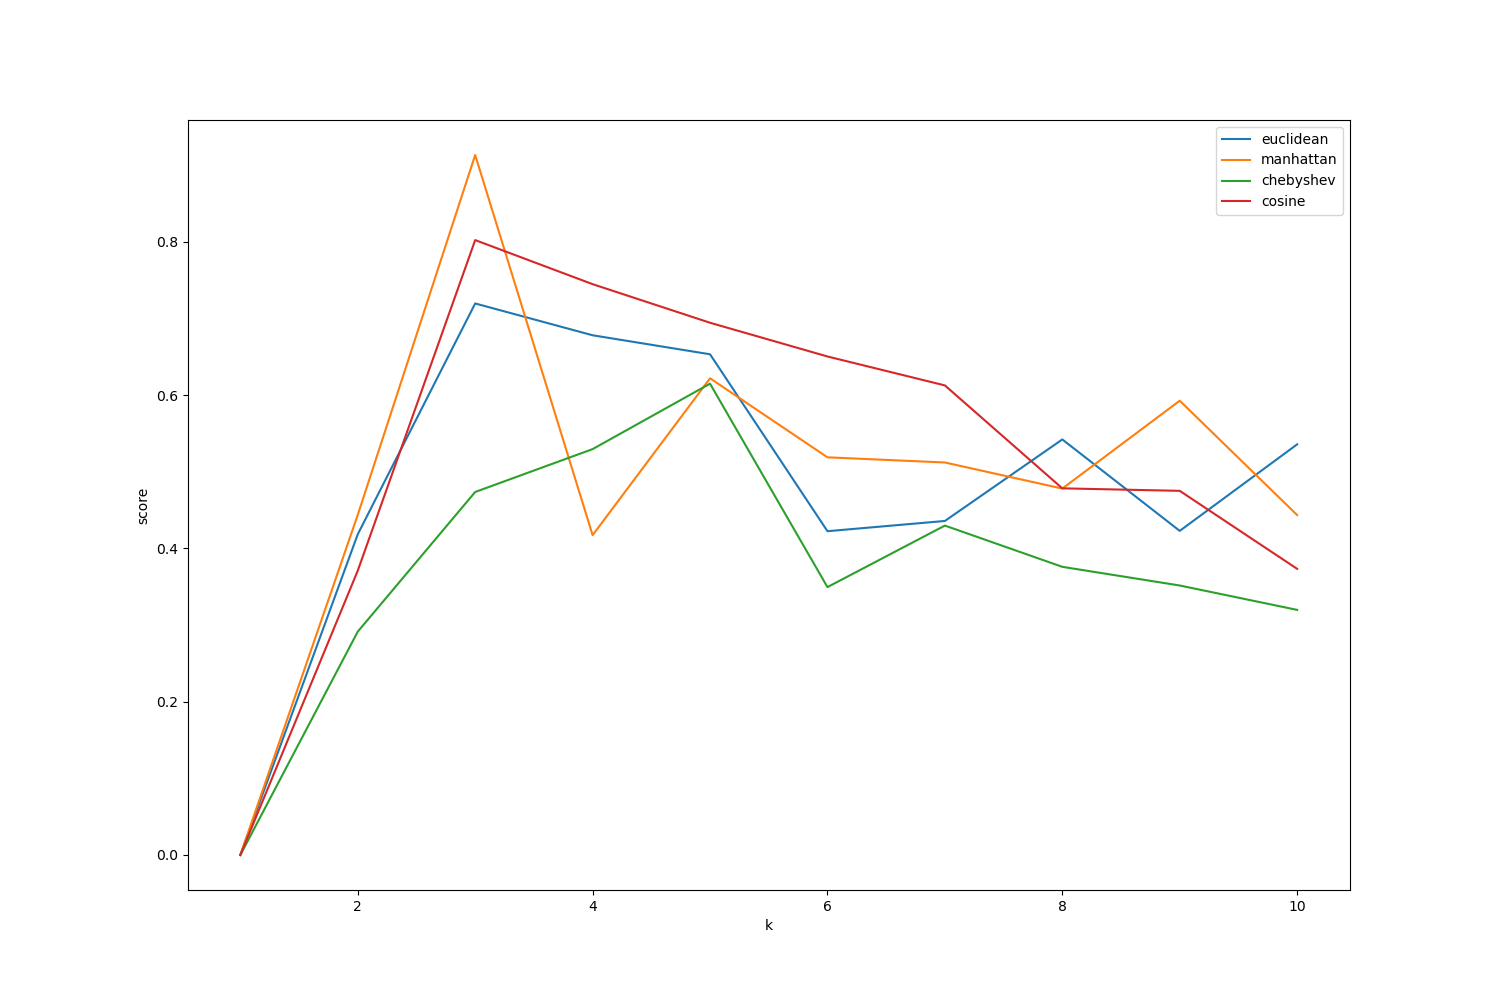
\includegraphics[width=0.45\textwidth]{../plots/wine/kmedians/ARI/k_1to10.png} }}%
	\qquad
	\subfloat[AMI ]{{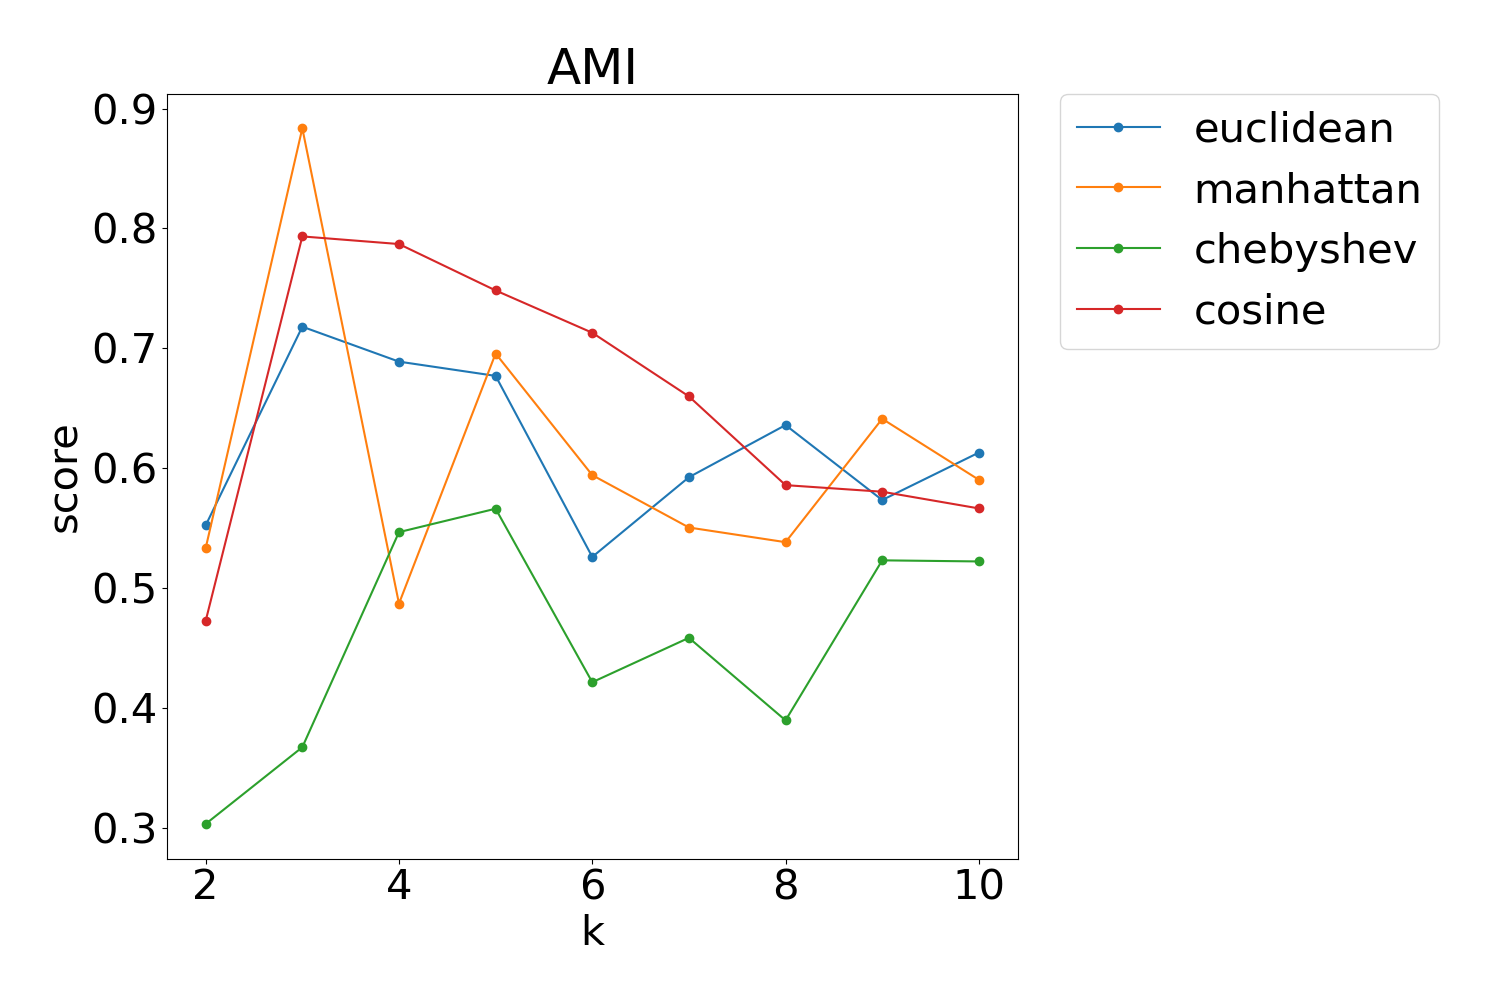
\includegraphics[width=0.45\textwidth]{../plots/wine/kmedians/AMI/k_1to10.png} }}%
	\qquad
	\subfloat[Completeness Score ]{{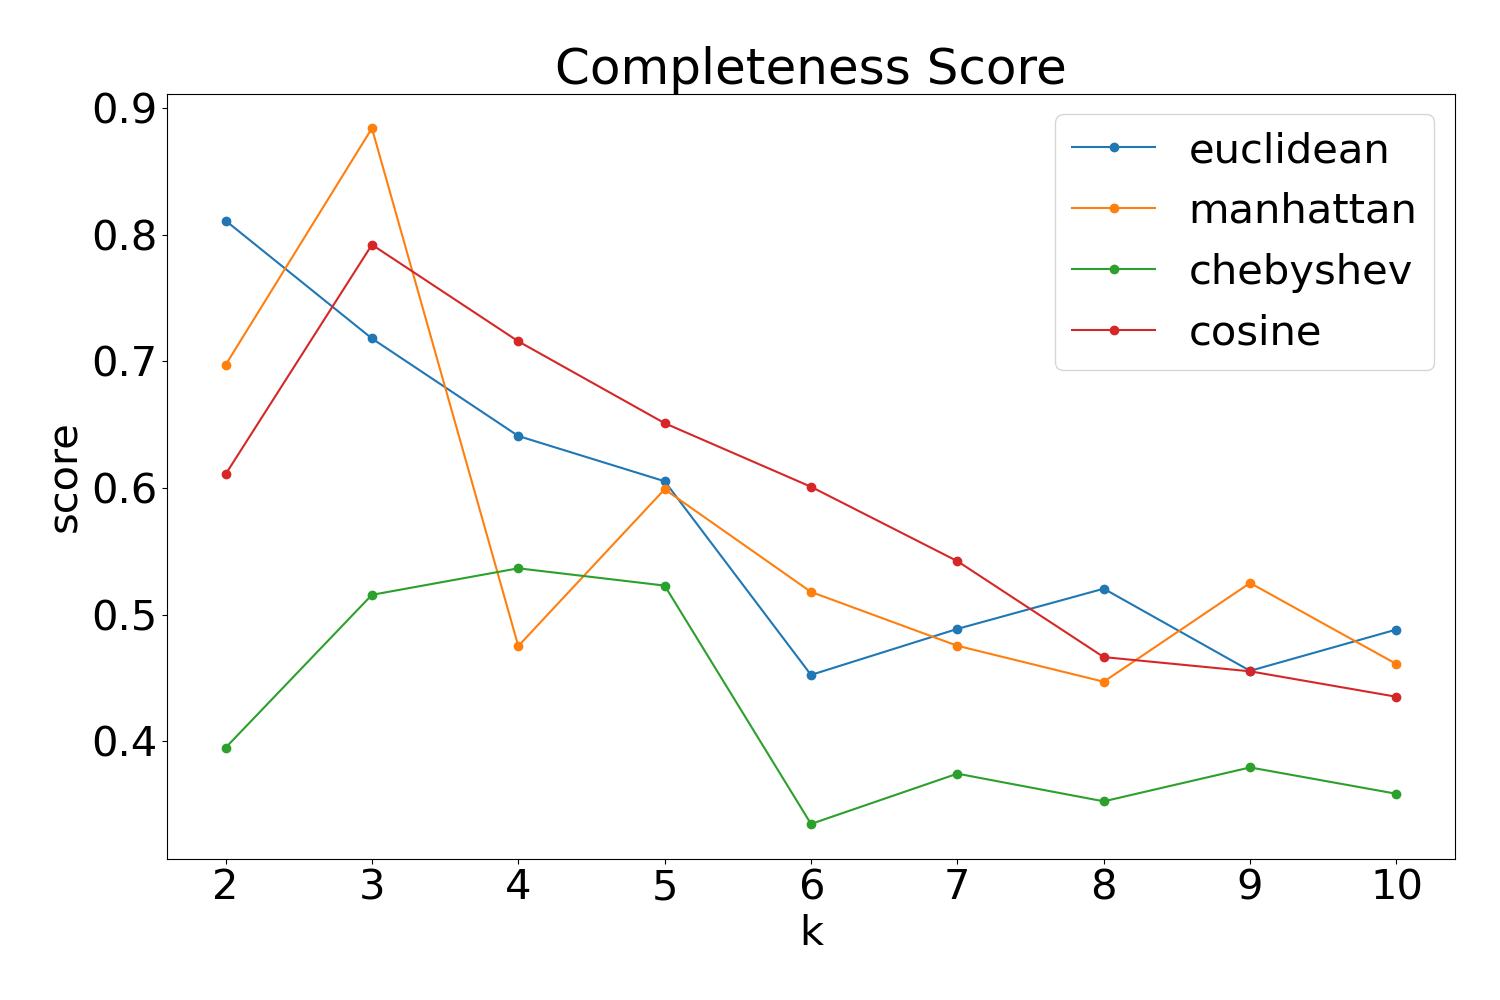
\includegraphics[width=0.45\textwidth]{../plots/wine/kmedians/Completeness Score/k_1to10.png} }}%
	\qquad
	\subfloat[Homogeneity Score ]{{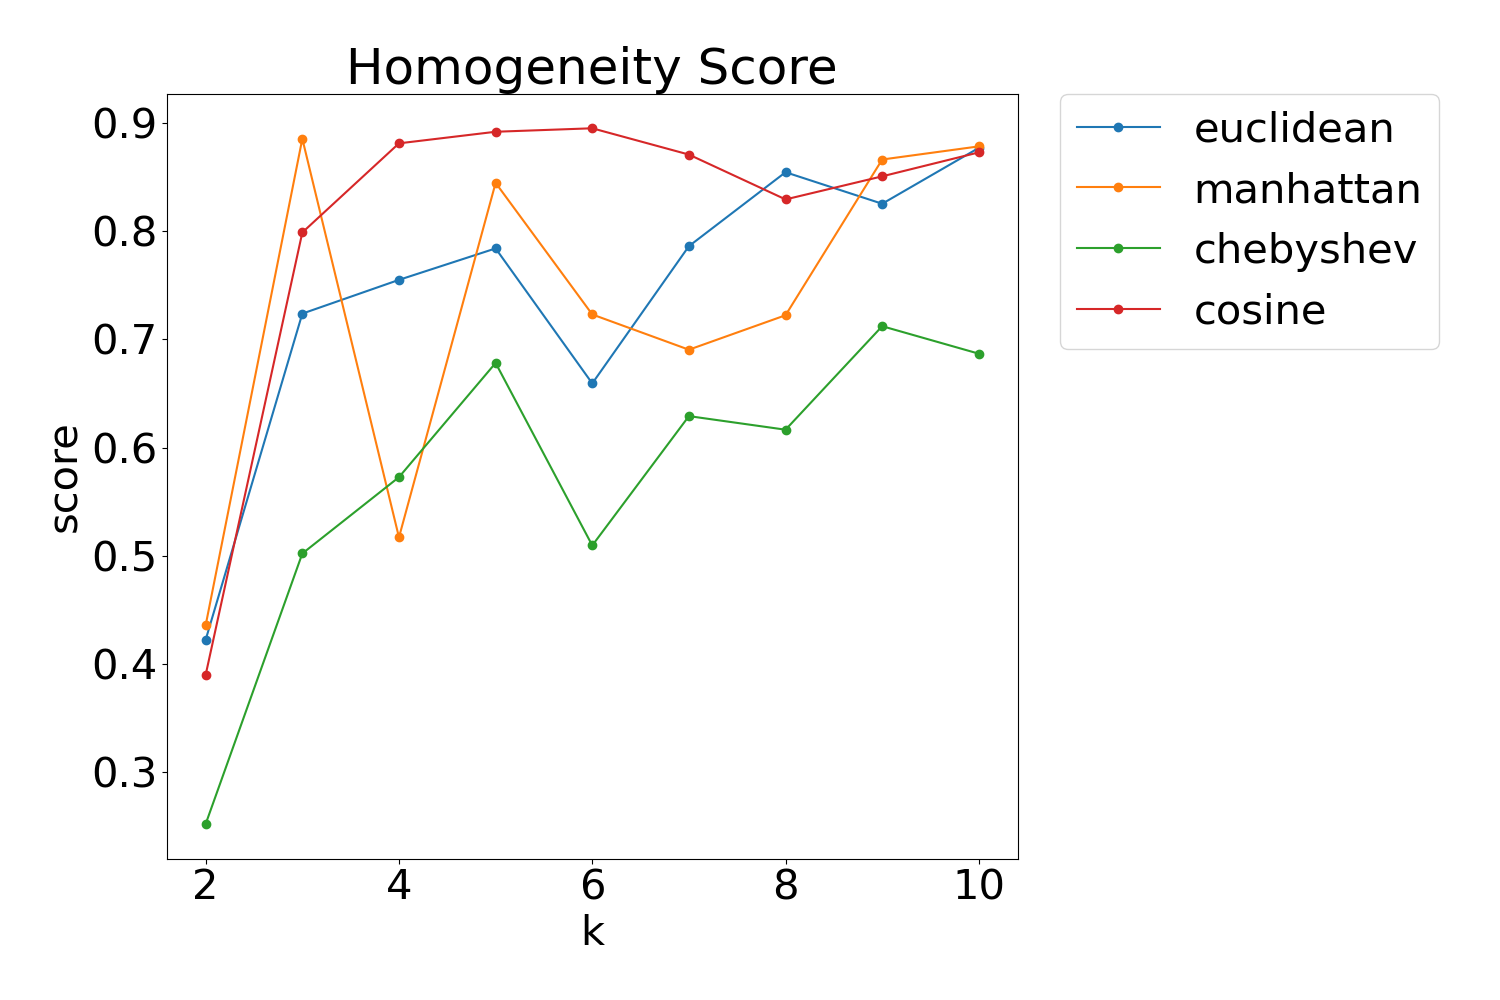
\includegraphics[width=0.45\textwidth]{../plots/wine/kmedians/Homogeneity Score/k_1to10.png} }}%
	\qquad
	\subfloat[Silhouette Score ]{{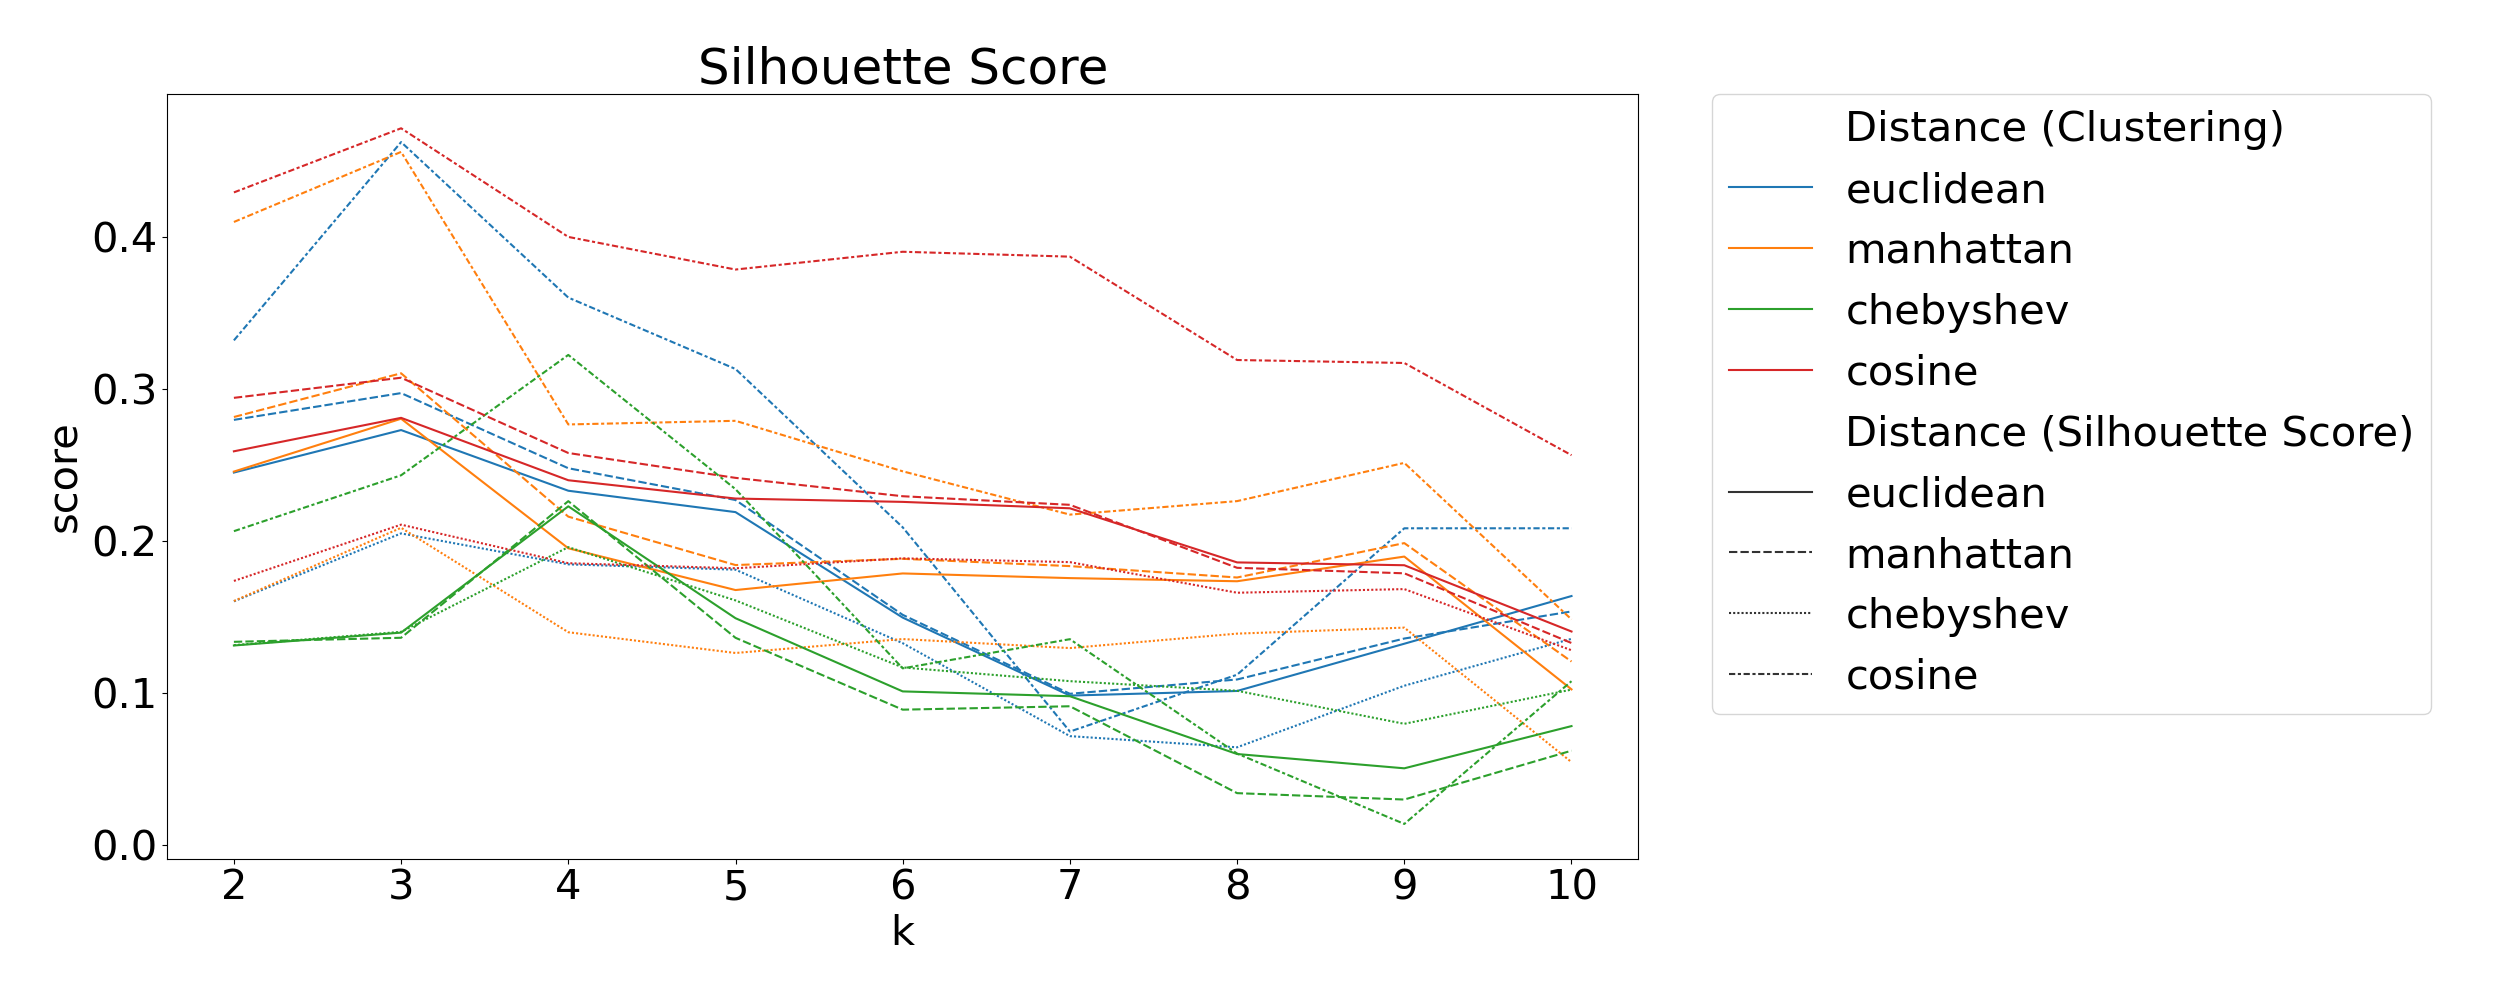
\includegraphics[width=1\textwidth]{../plots/wine/kmedians/Silhouette Score/k_1to10.png} }}%
	
	\caption{Comparison of clustering scores for K-Medians-clustering on Wine dataset}%
	\label{fig:kmedians_wine}
\end{figure}

\begin{figure}[H]
	\centering
	\subfloat[Silhouette Score ]{{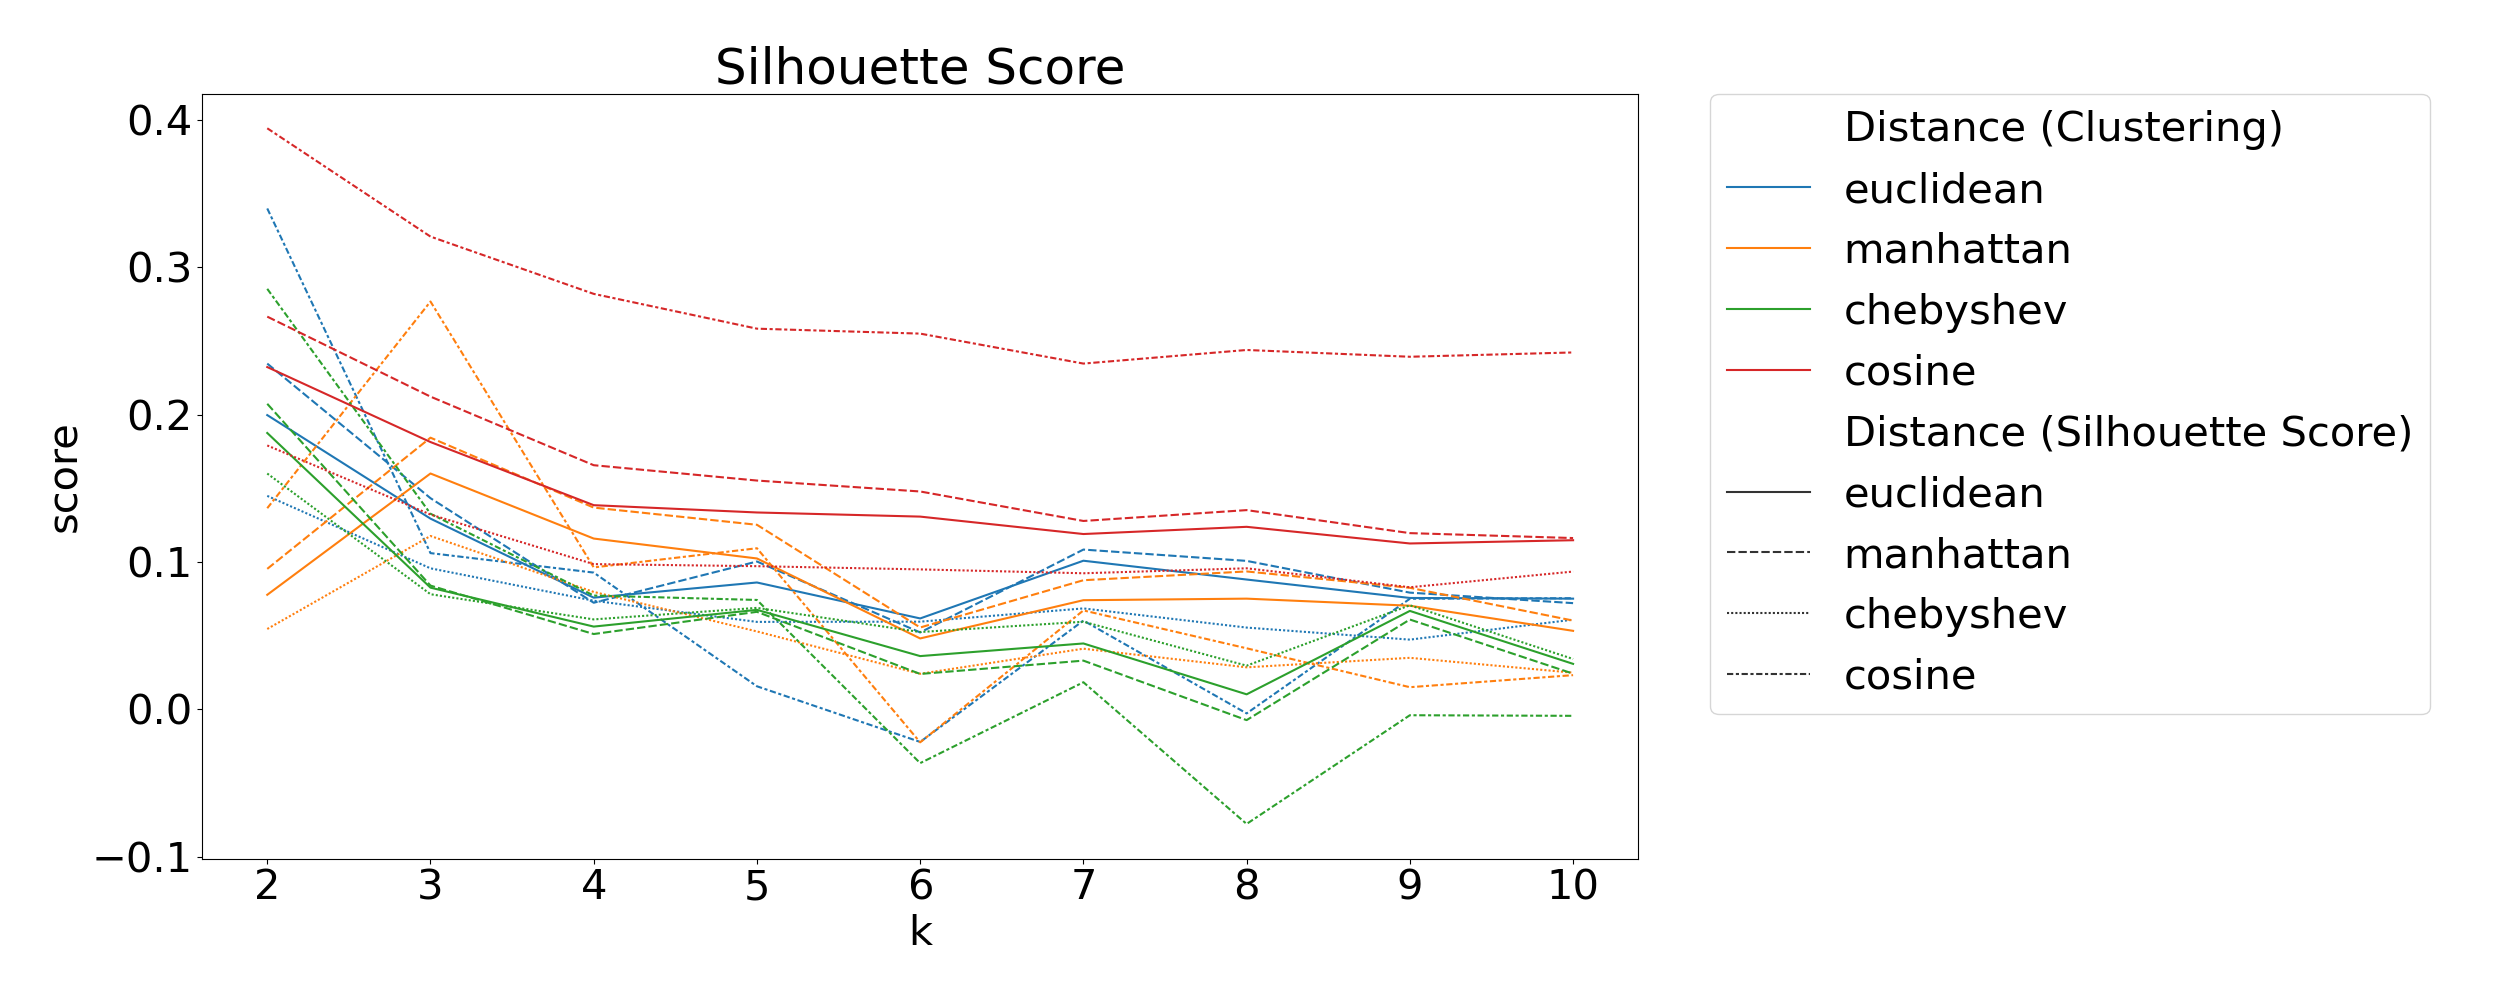
\includegraphics[width=1\textwidth]{../plots/diabetes/kmedians/Silhouette Score/k_1to10.png} }}%
	
	\caption{Comparison of clustering scores for K-Medians-clustering on Diabetes dataset}%
	\label{fig:kmedians_diabetes}
\end{figure}

\begin{figure}[H]
	\centering
	\subfloat[ARI ]{{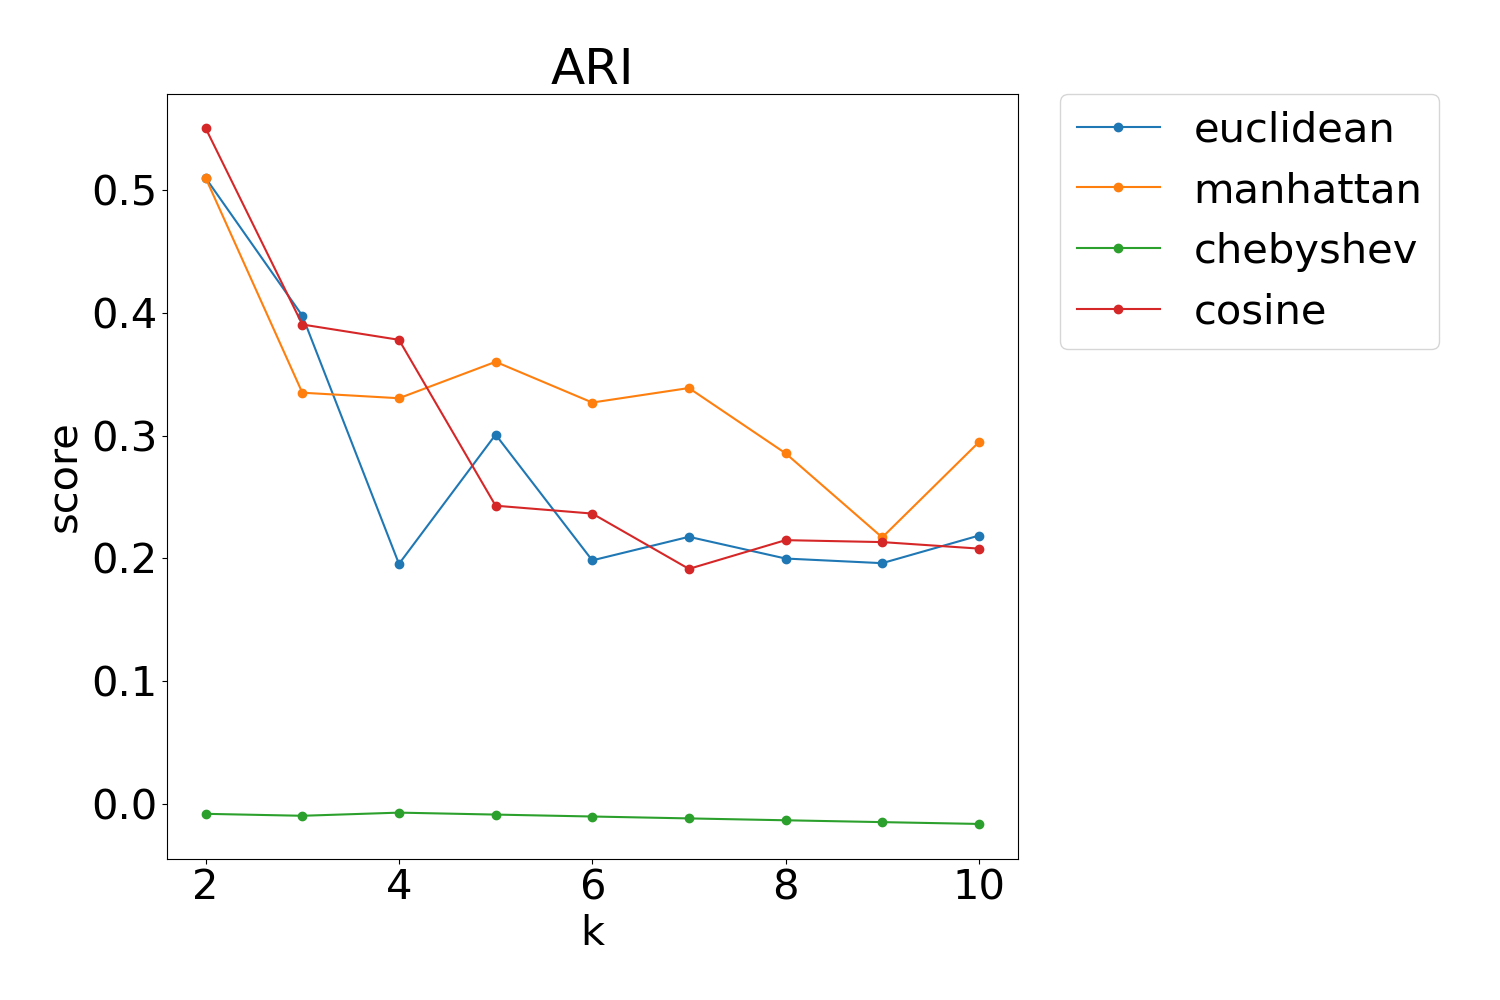
\includegraphics[width=0.45\textwidth]{../plots/housevotes/kmedians/ARI/k_1to10.png} }}%
	\qquad
	\subfloat[AMI ]{{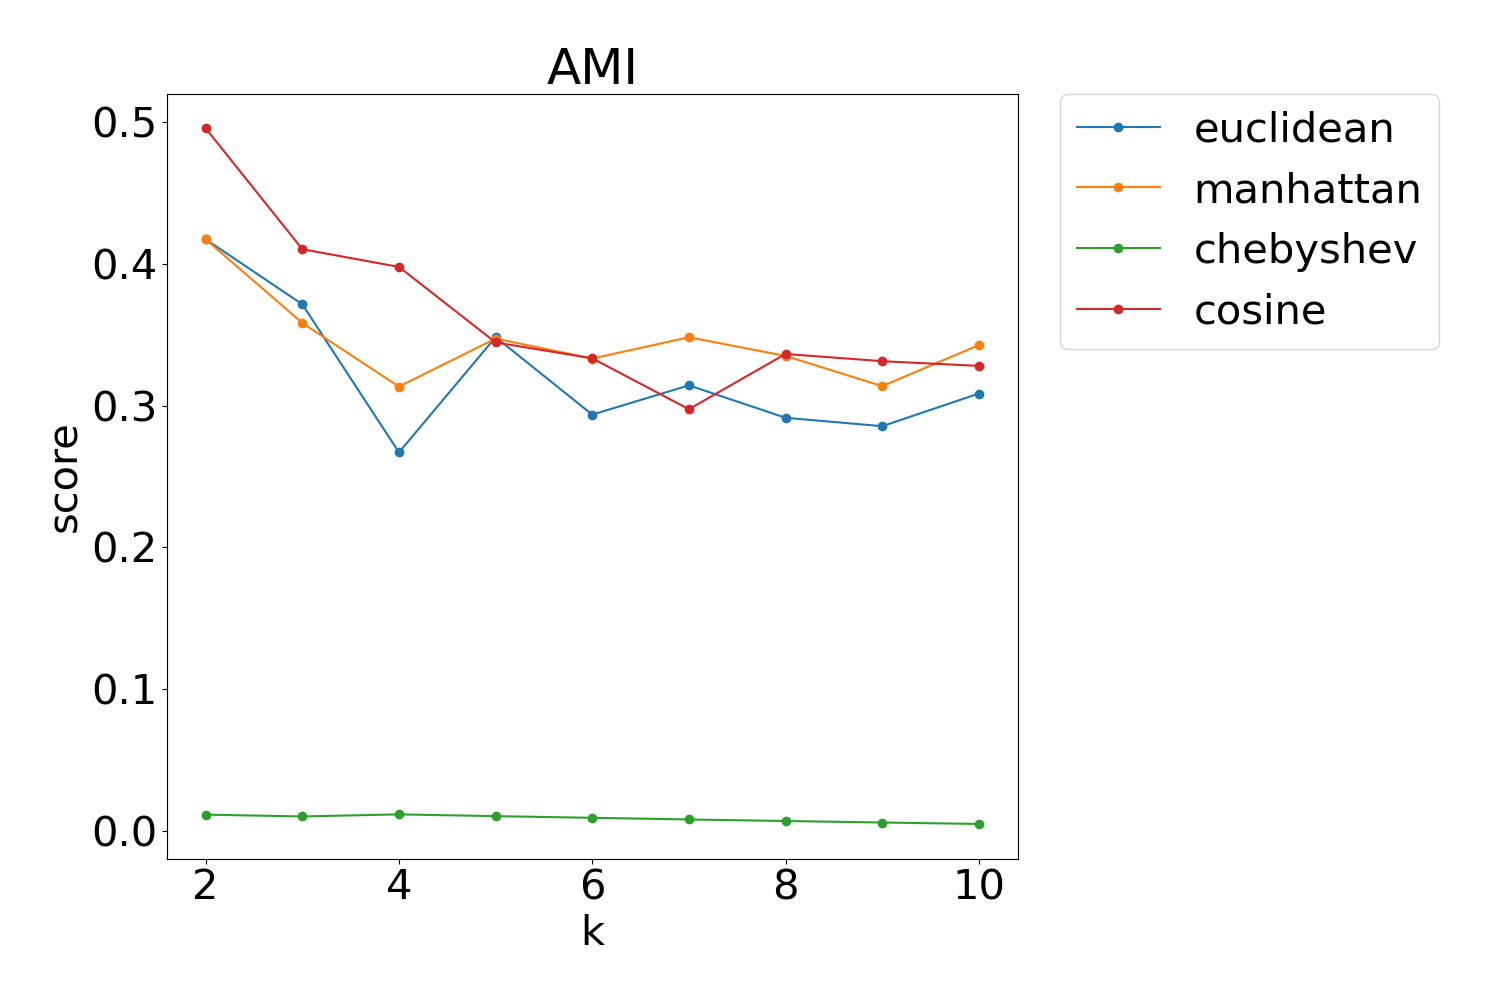
\includegraphics[width=0.45\textwidth]{../plots/housevotes/kmedians/AMI/k_1to10.png} }}%
	\qquad
	\subfloat[Completeness Score ]{{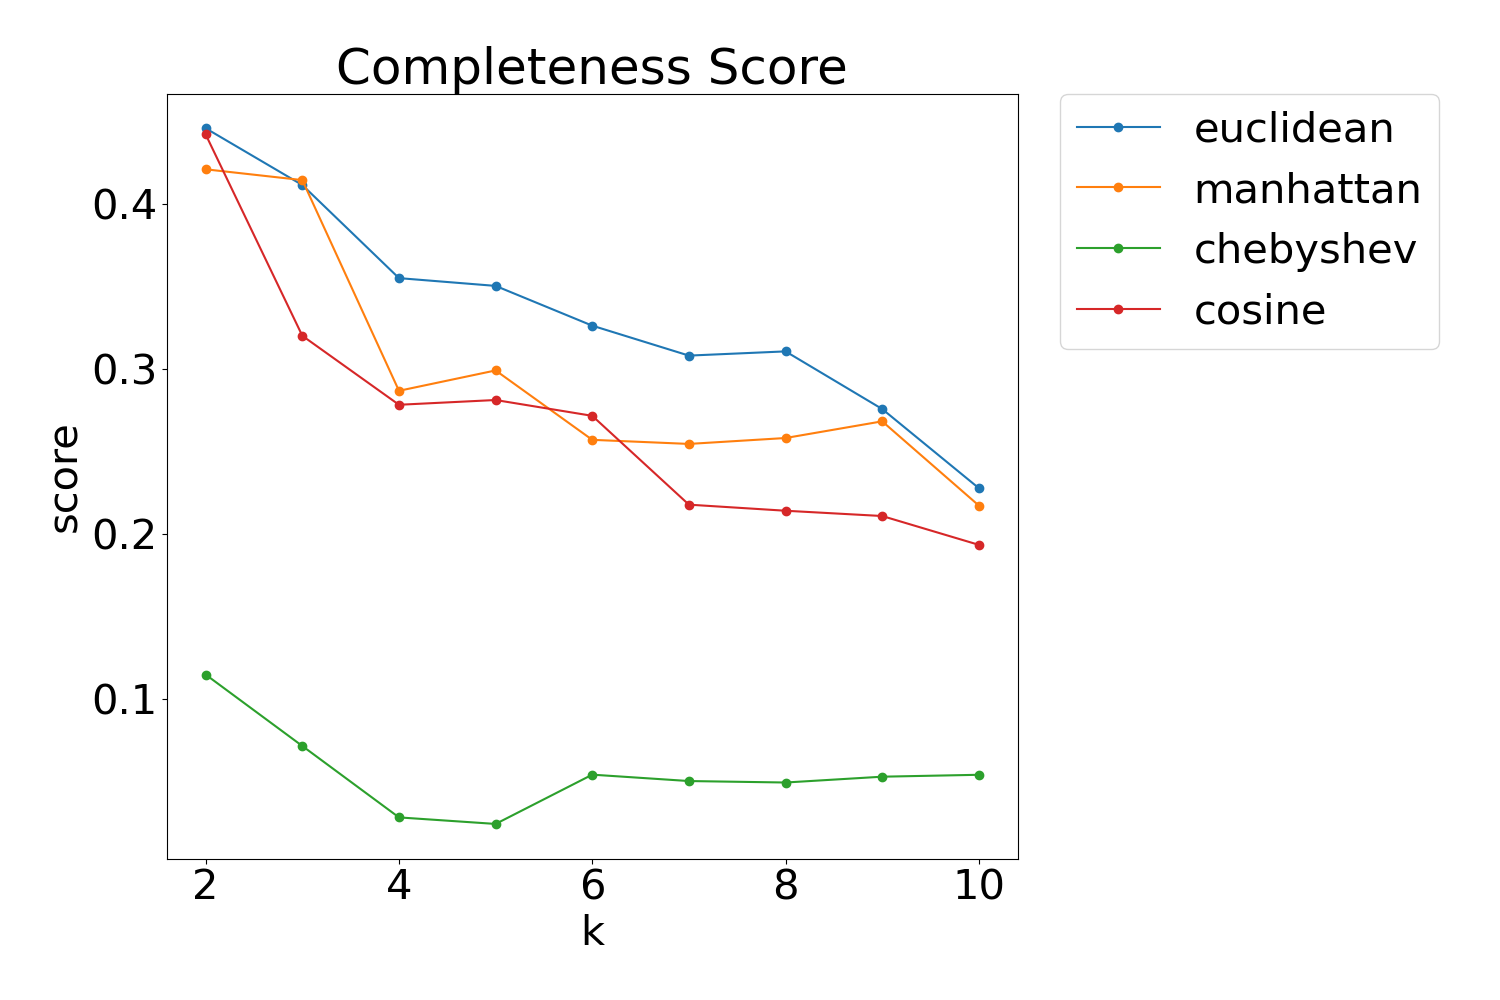
\includegraphics[width=0.45\textwidth]{../plots/housevotes/kmedians/Completeness Score/k_1to10.png} }}%
	\qquad
	\subfloat[Homogeneity Score ]{{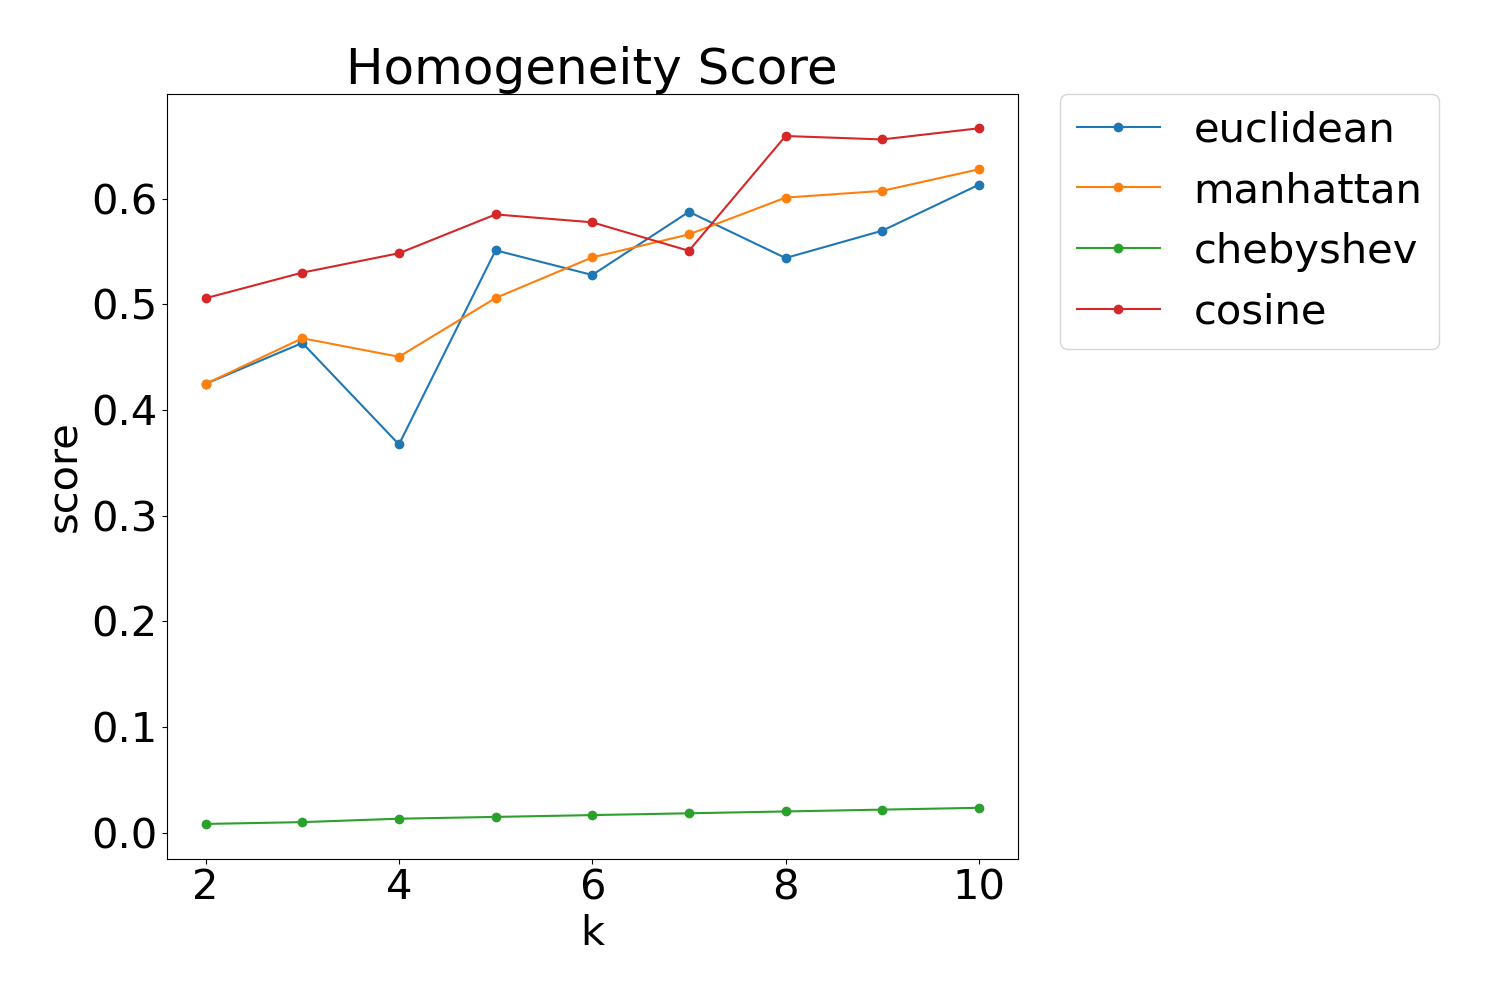
\includegraphics[width=0.45\textwidth]{../plots/housevotes/kmedians/Homogeneity Score/k_1to10.png} }}%
	\qquad
	\subfloat[Silhouette Score ]{{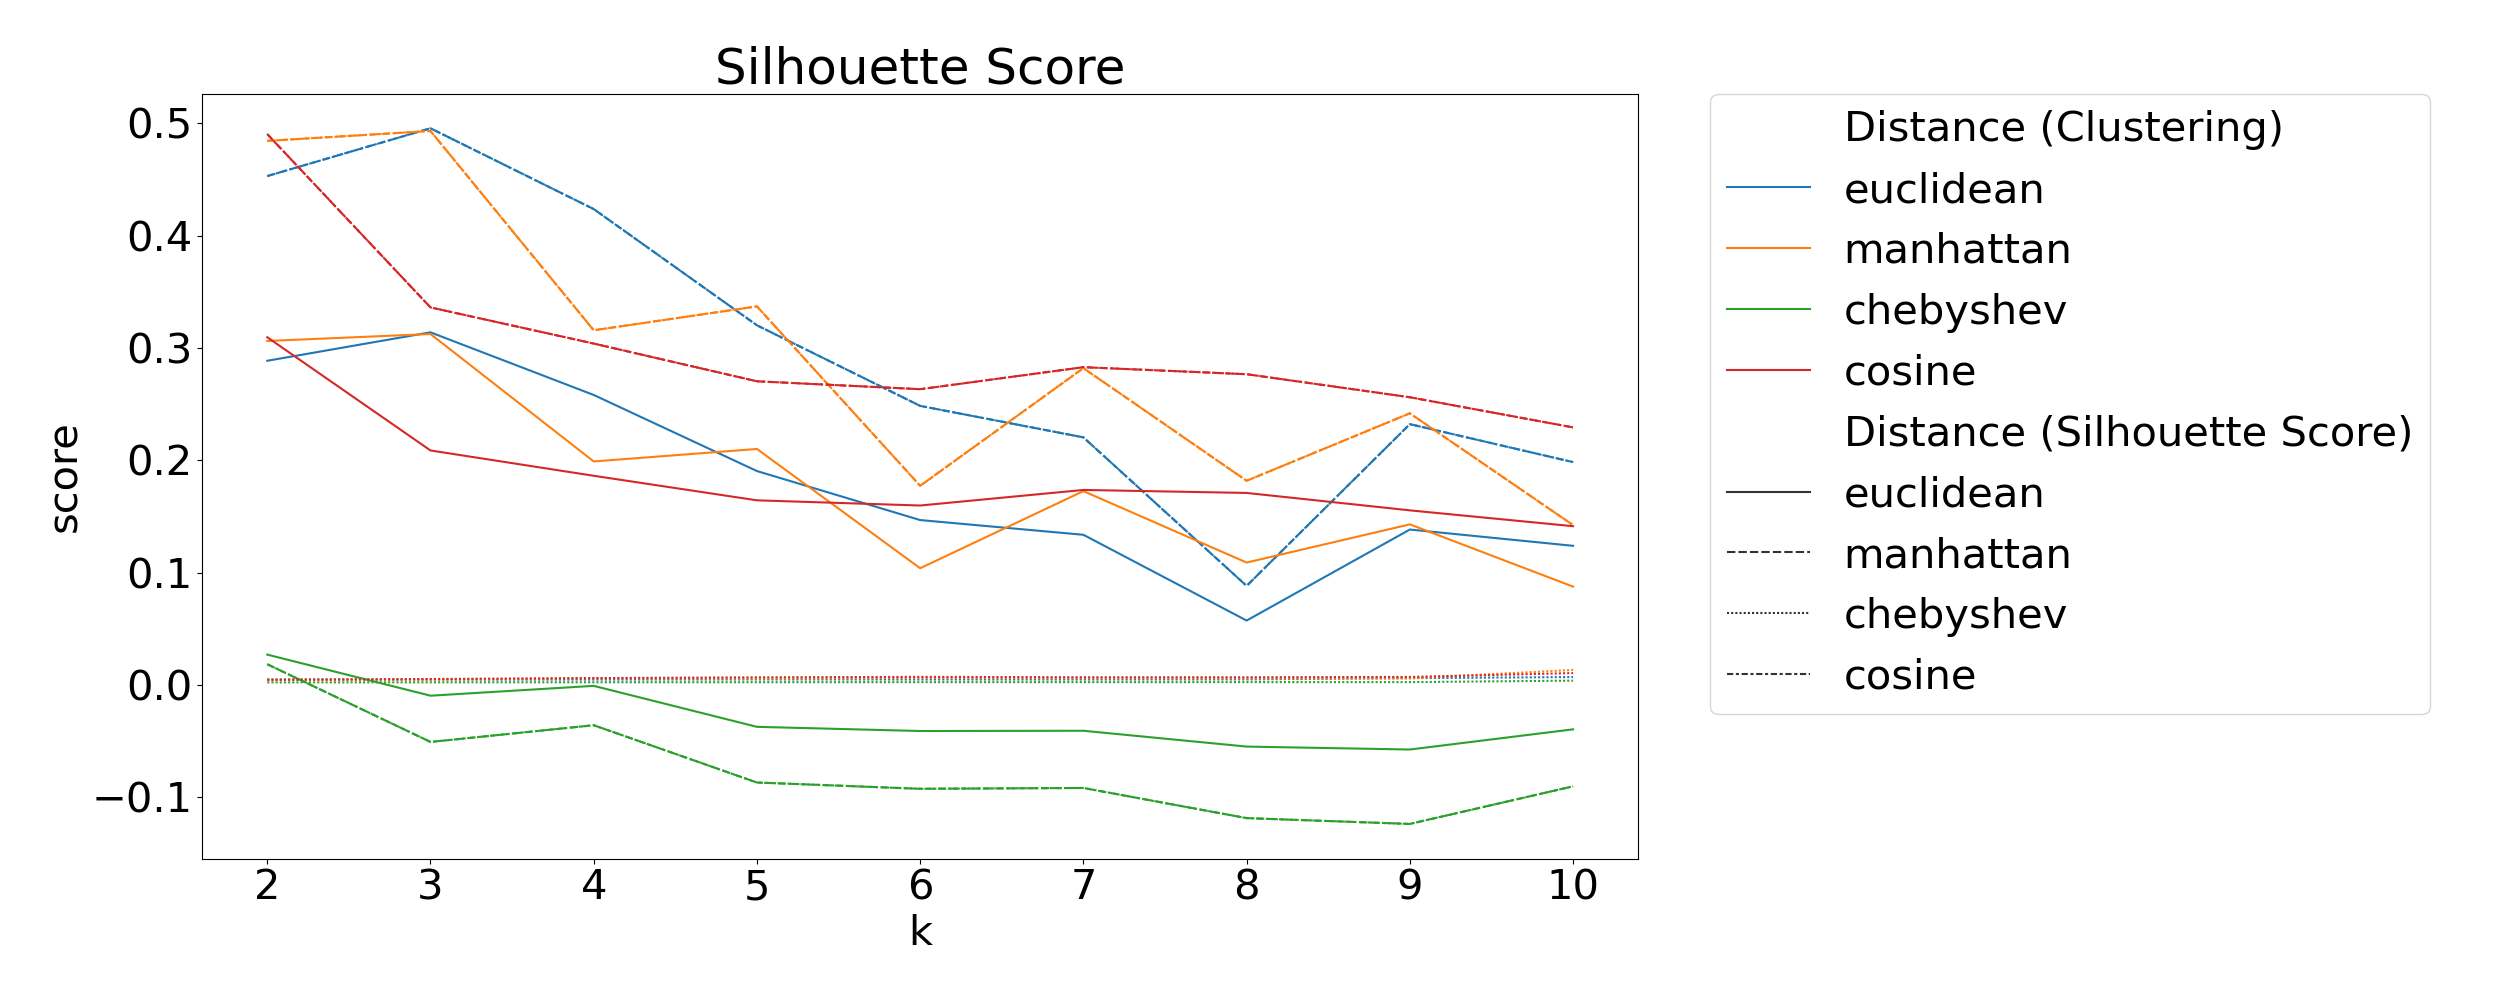
\includegraphics[width=1\textwidth]{../plots/housevotes/kmedians/Silhouette Score/k_1to10.png} }}%
	
	\caption{Comparison of clustering scores for K-Medians-clustering on Housevotes dataset}%
	\label{fig:kmedians_housevotes}
\end{figure}

\begin{figure}[H]
	\centering
	\subfloat[ARI ]{{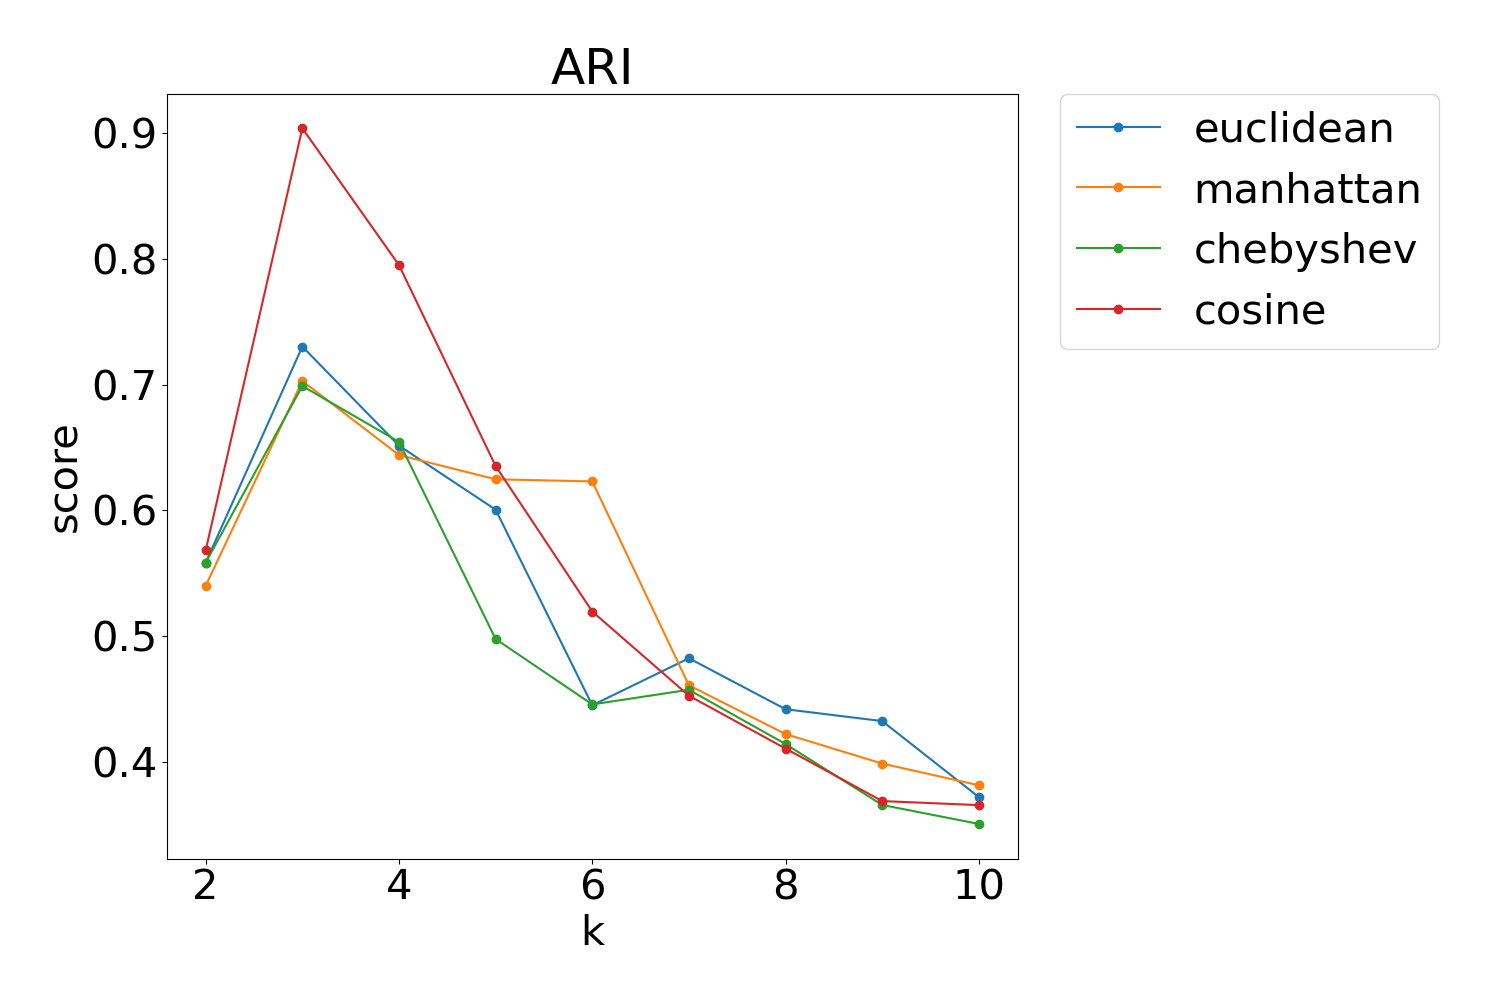
\includegraphics[width=0.45\textwidth]{../plots/iris/kmedoids/ARI/k_1to10.png} }}%
	\qquad
	\subfloat[AMI ]{{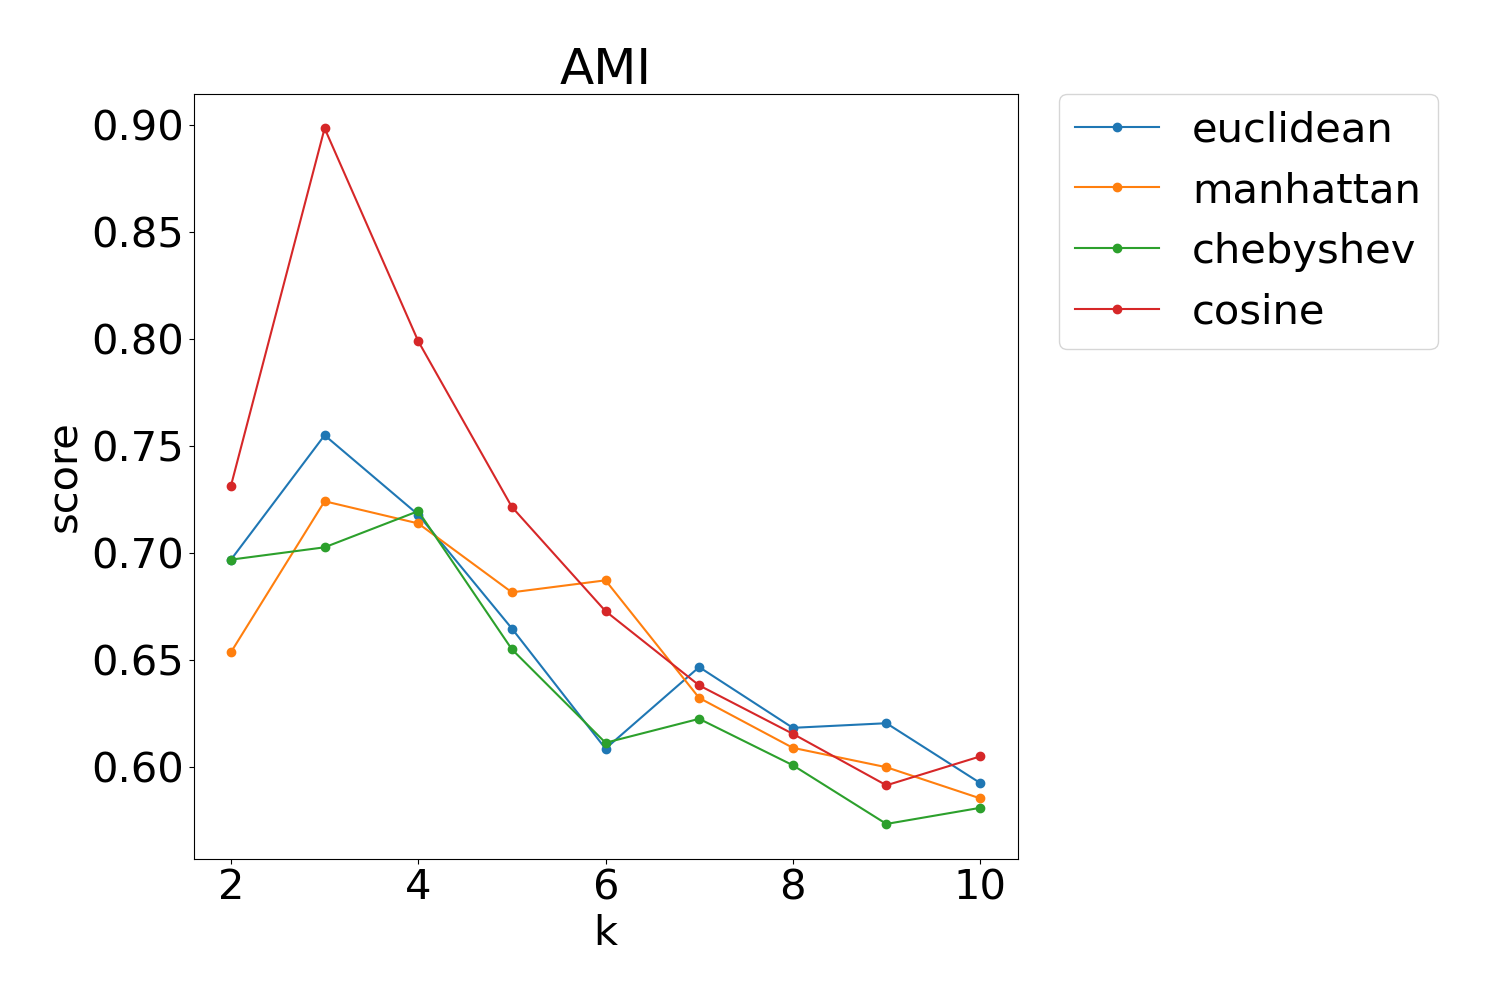
\includegraphics[width=0.45\textwidth]{../plots/iris/kmedoids/AMI/k_1to10.png} }}%
	\qquad
	\subfloat[Completeness Score ]{{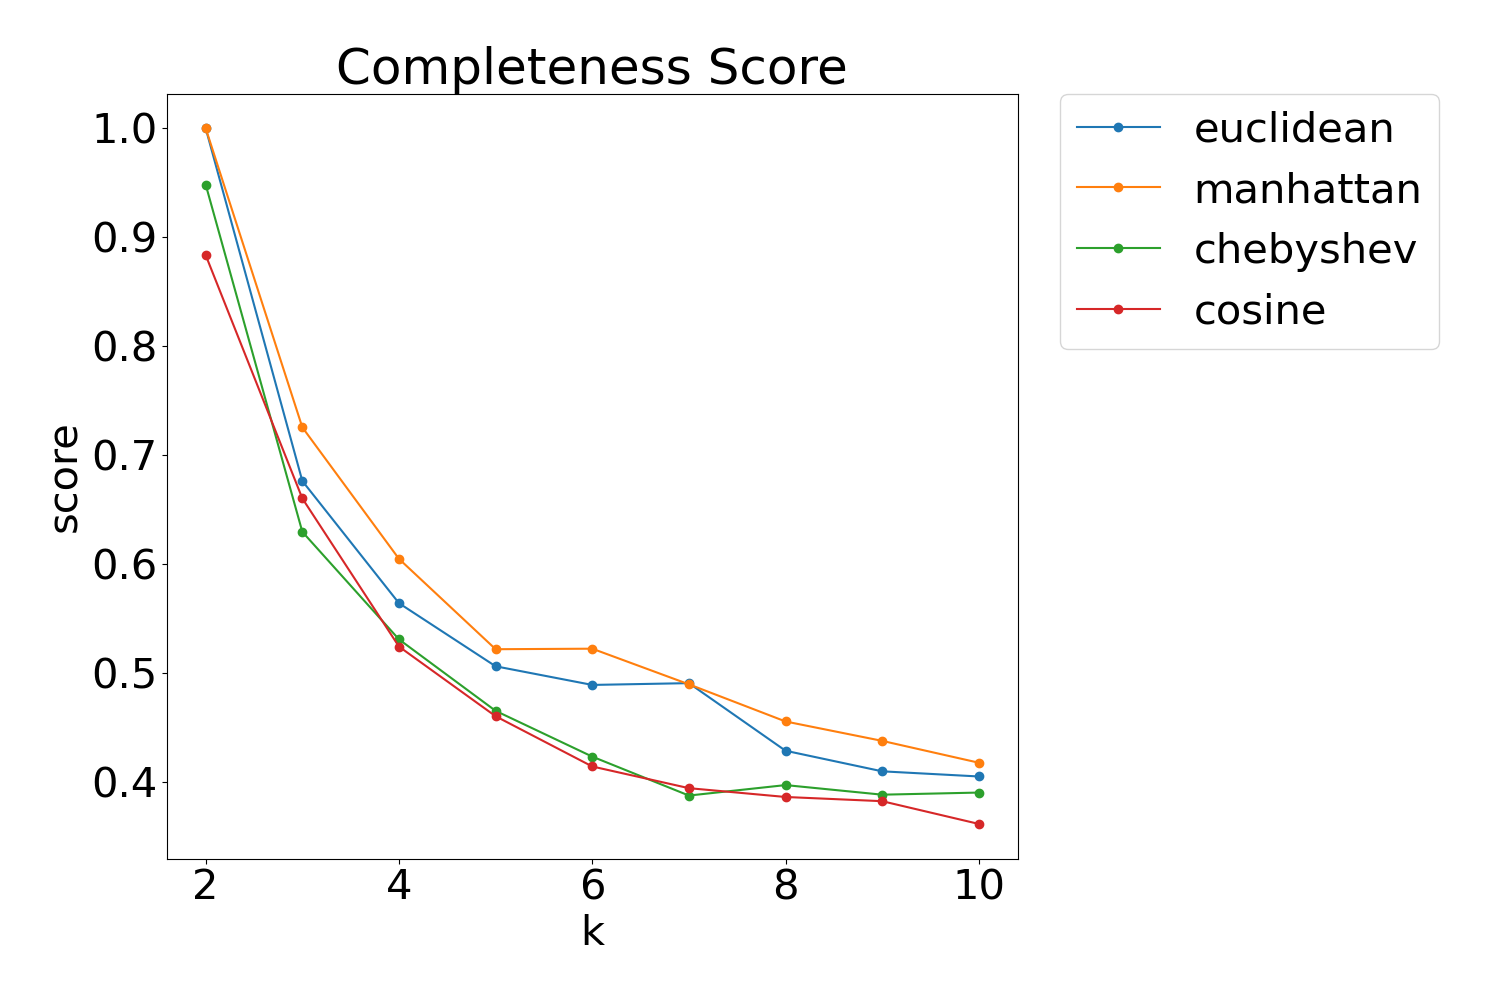
\includegraphics[width=0.45\textwidth]{../plots/iris/kmedoids/Completeness Score/k_1to10.png} }}%
	\qquad
	\subfloat[Homogeneity Score ]{{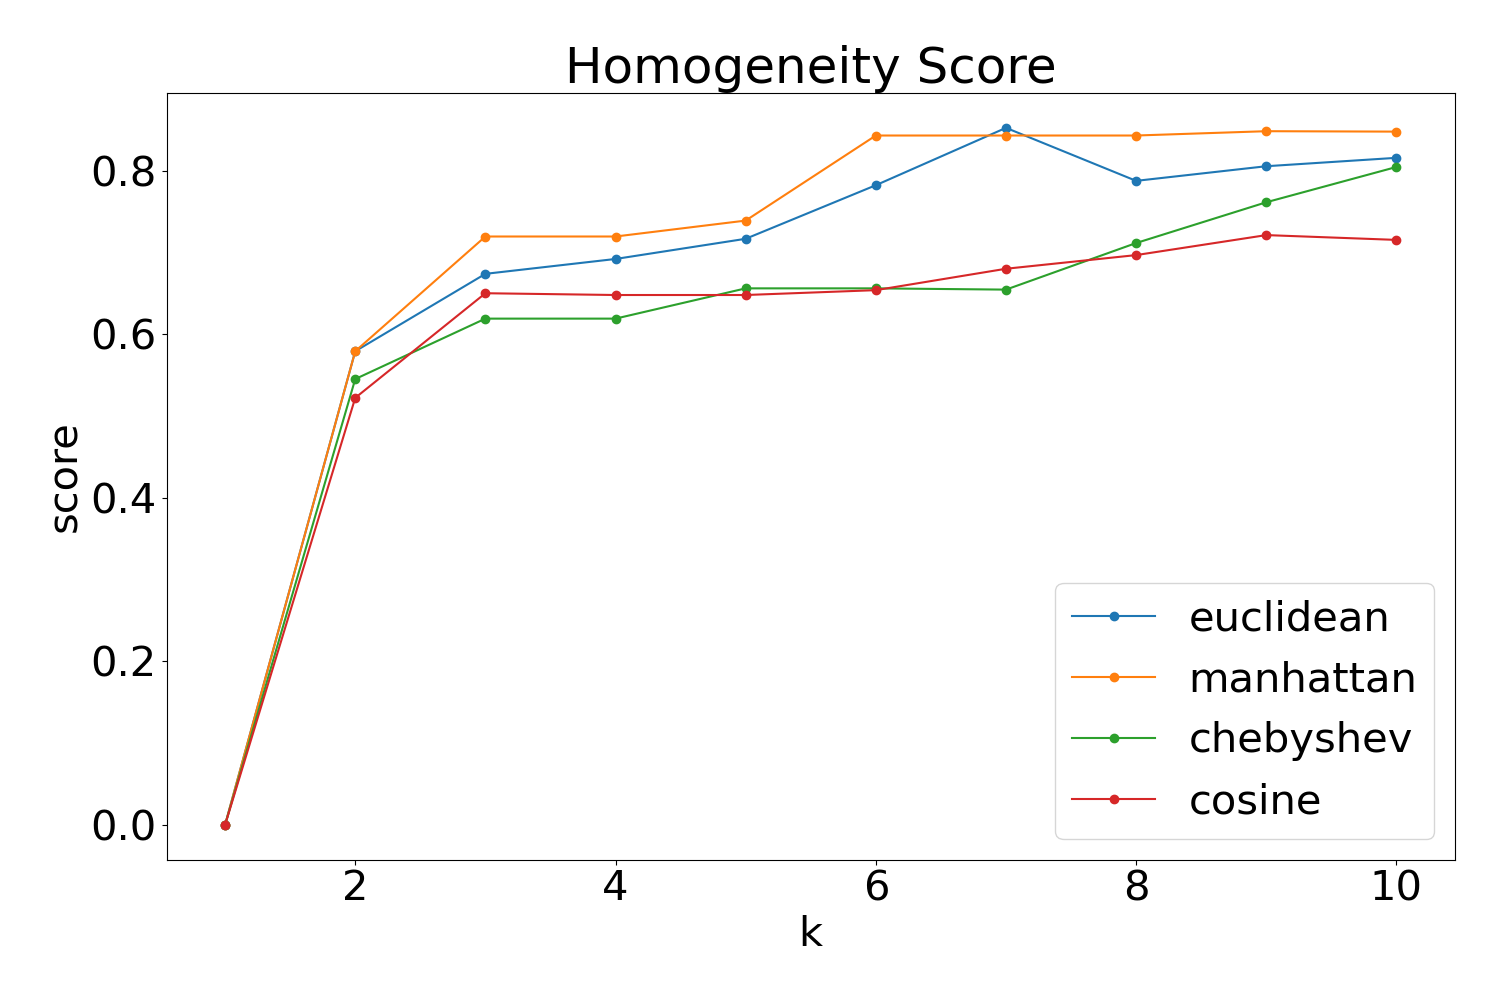
\includegraphics[width=0.45\textwidth]{../plots/iris/kmedoids/Homogeneity Score/k_1to10.png} }}%
	\qquad
	\subfloat[Silhouette Score ]{{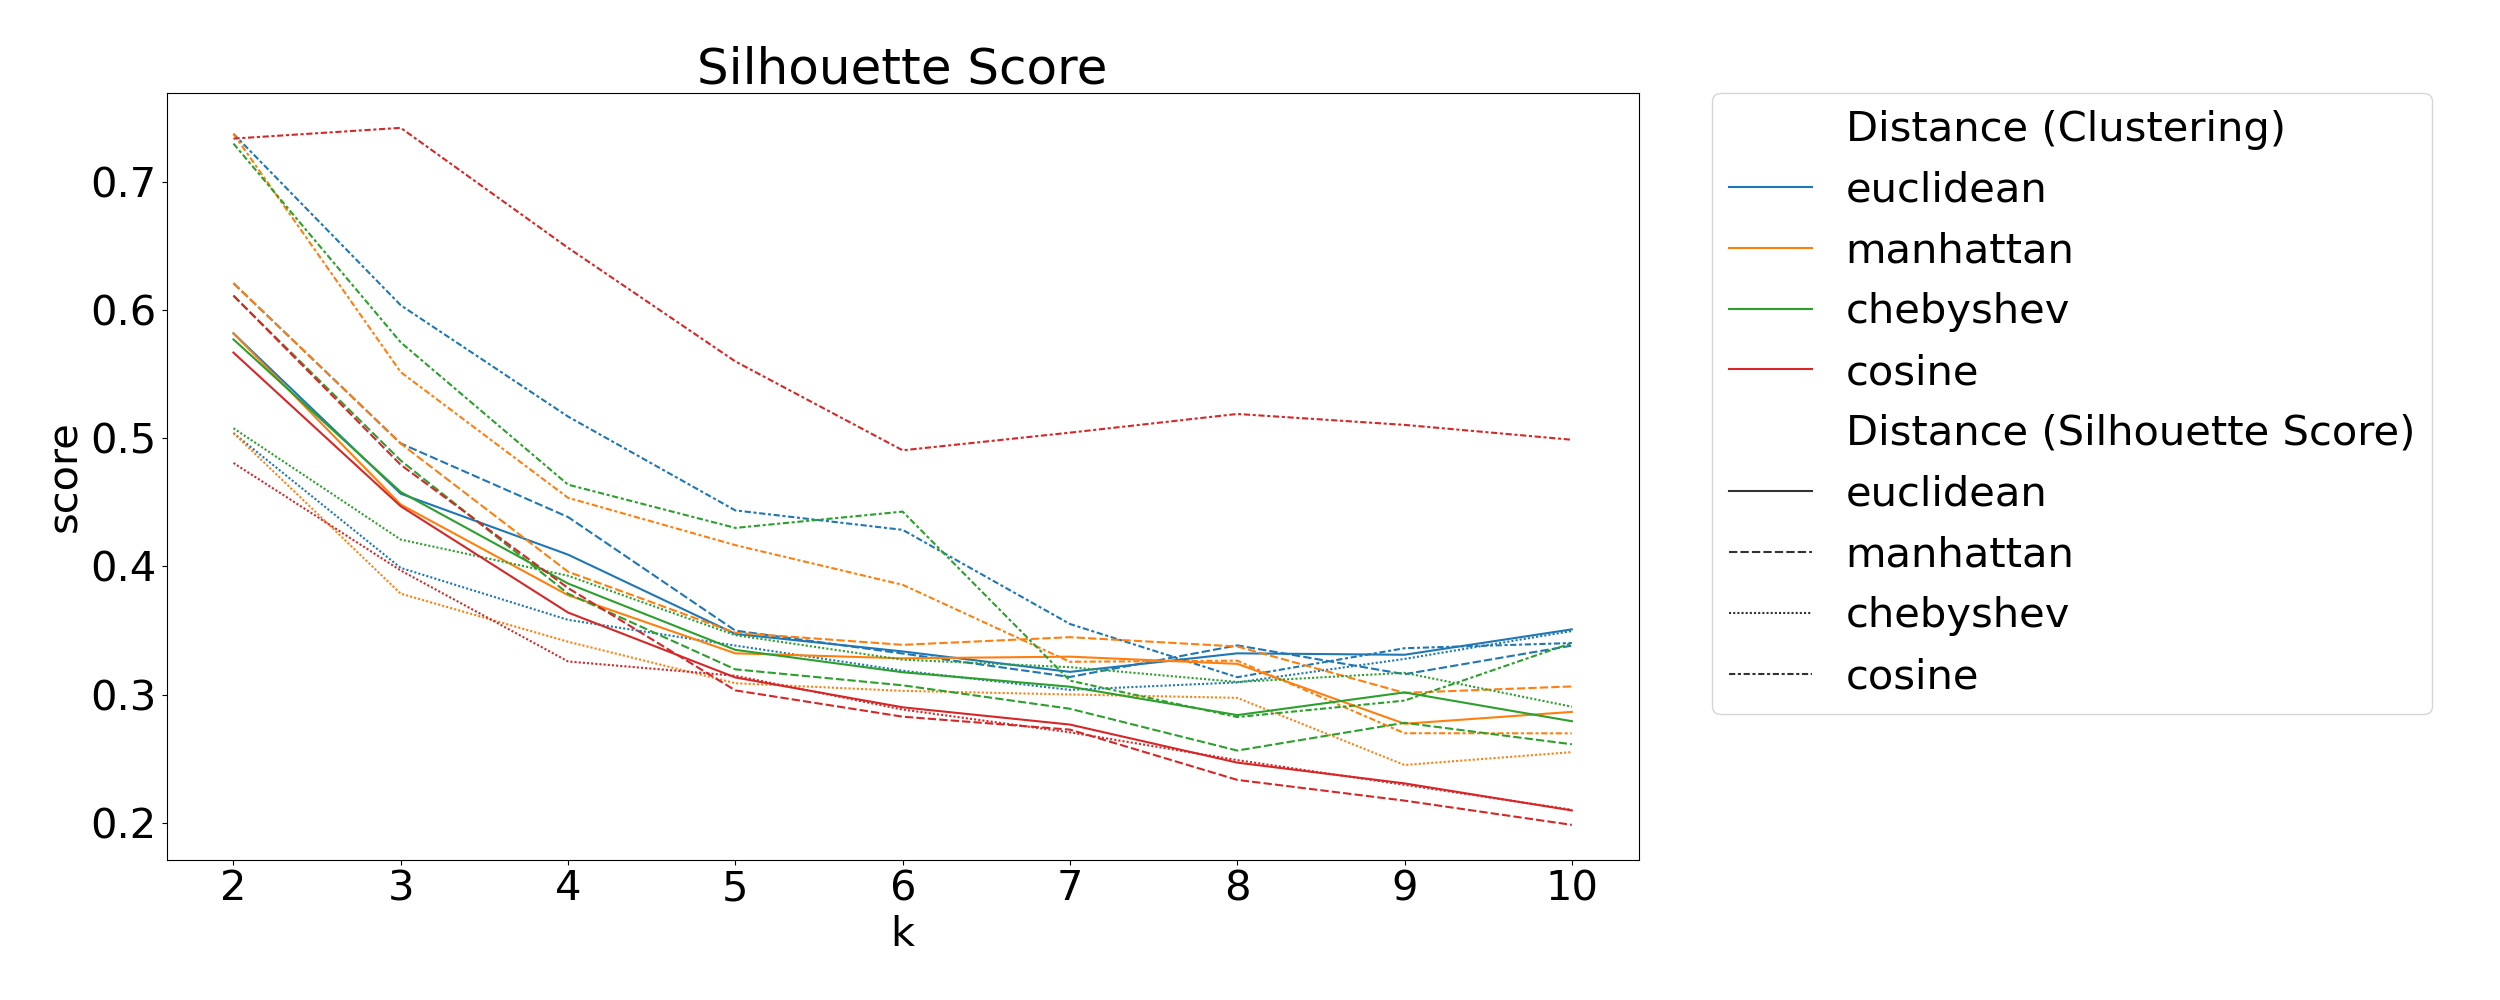
\includegraphics[width=1\textwidth]{../plots/iris/kmedoids/Silhouette Score/k_1to10.png} }}%
	
	\caption{Comparison of clustering scores for K-Medoids-clustering on Iris dataset}%
	\label{fig:kmedoids_iris}
\end{figure}

\begin{figure}[H]
	\centering
	\subfloat[ARI ]{{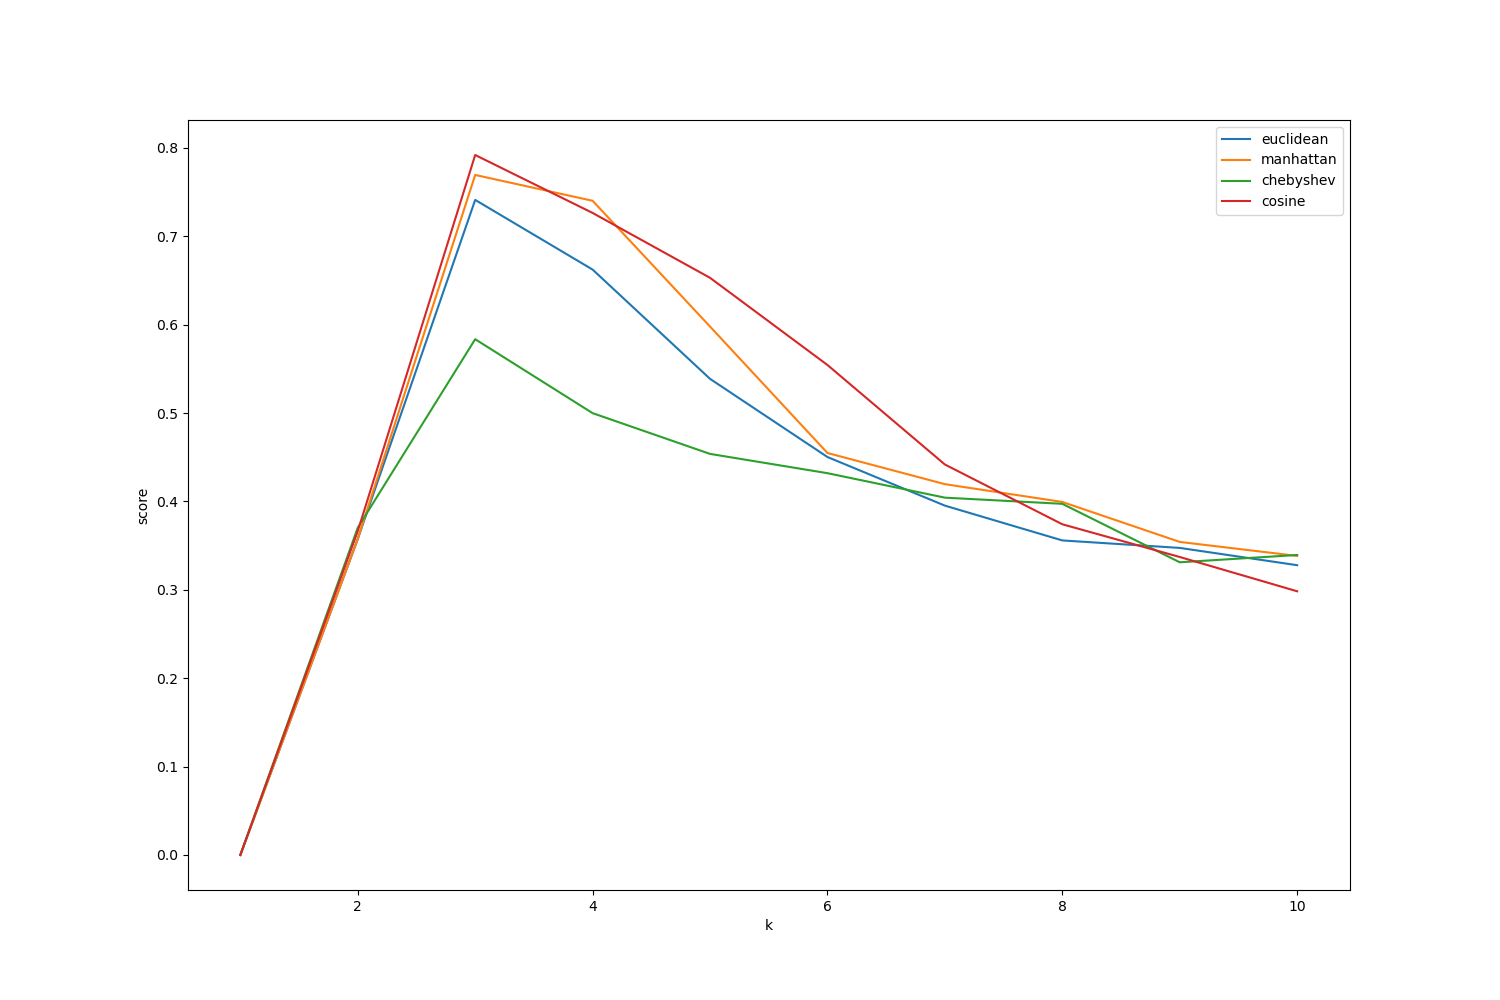
\includegraphics[width=0.45\textwidth]{../plots/wine/kmedoids/ARI/k_1to10.png} }}%
	\qquad
	\subfloat[AMI ]{{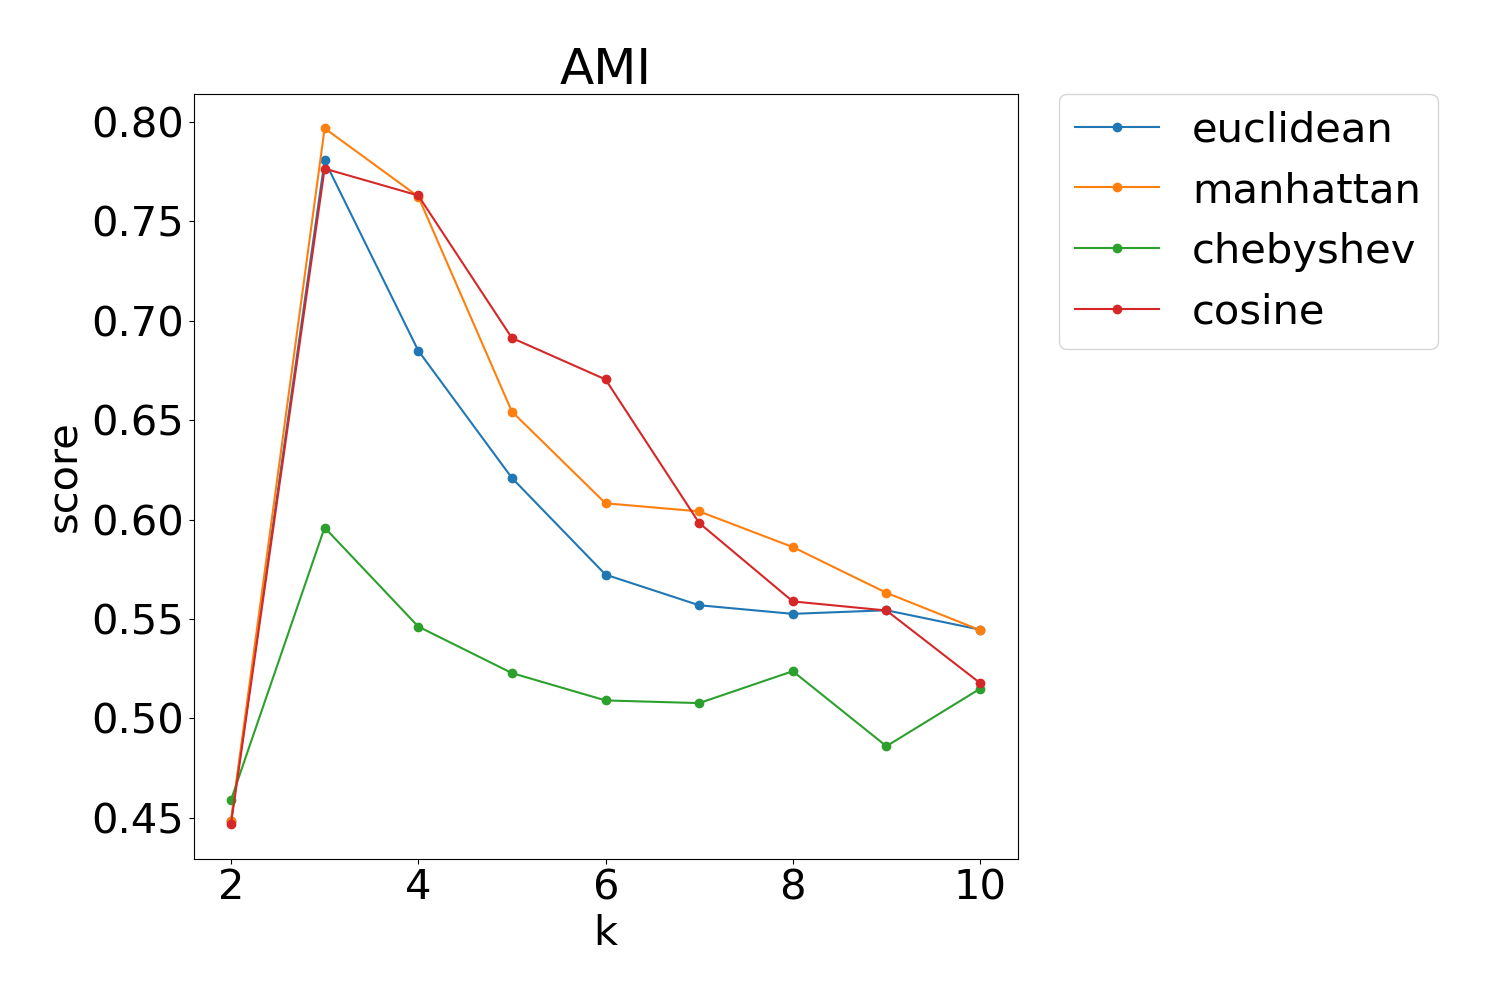
\includegraphics[width=0.45\textwidth]{../plots/wine/kmedoids/AMI/k_1to10.png} }}%
	\qquad
	\subfloat[Completeness Score ]{{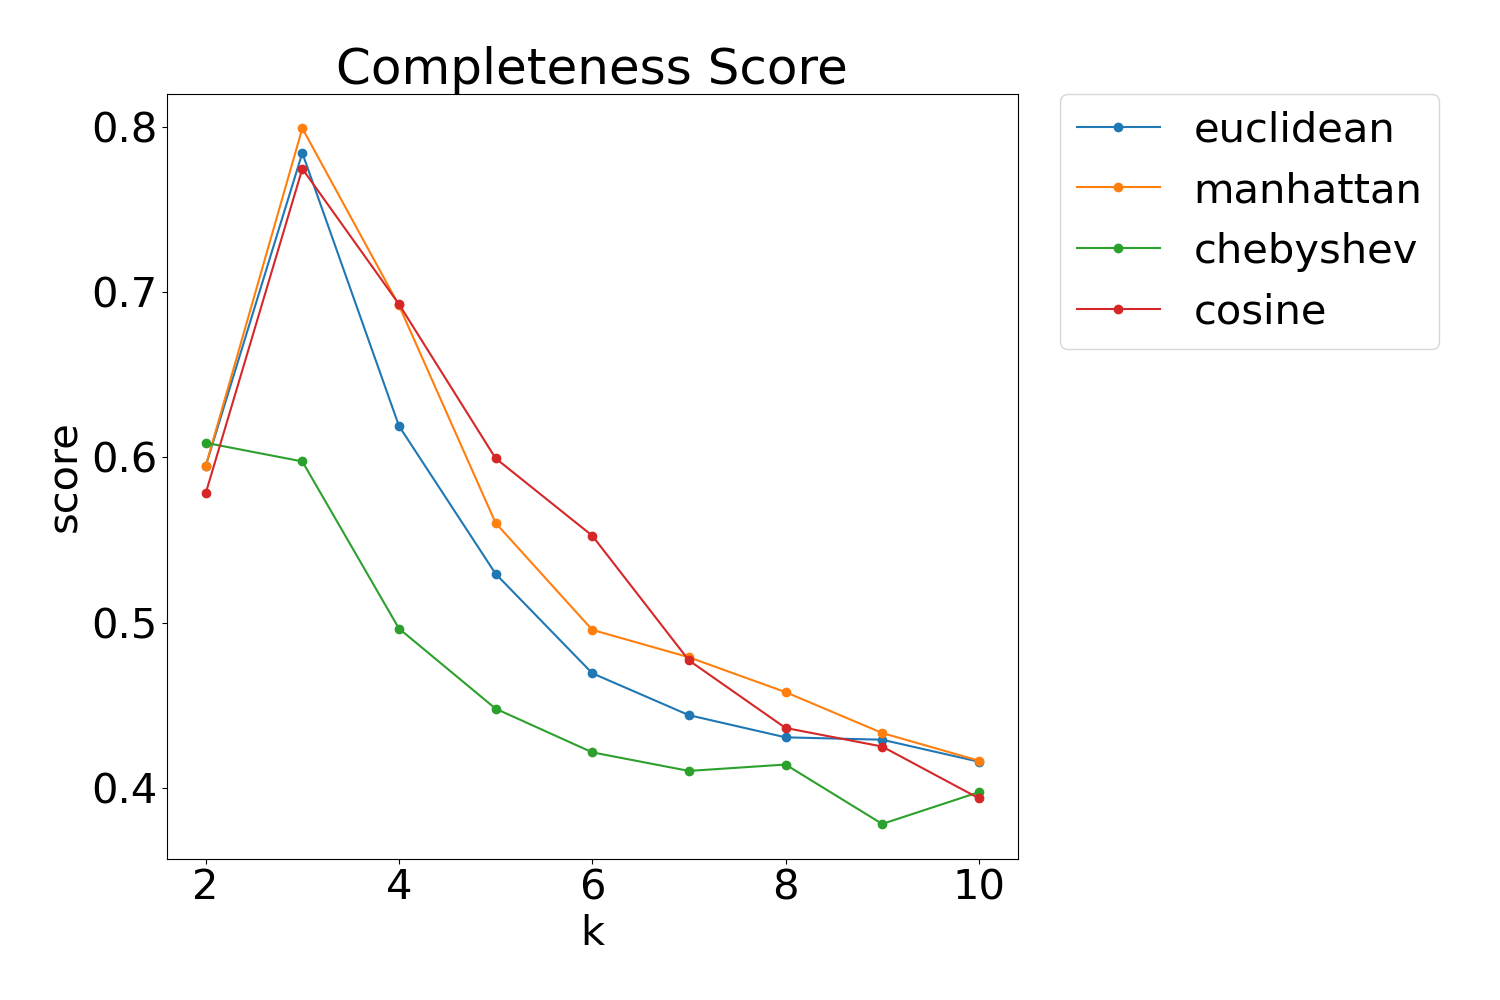
\includegraphics[width=0.45\textwidth]{../plots/wine/kmedoids/Completeness Score/k_1to10.png} }}%
	\qquad
	\subfloat[Homogeneity Score ]{{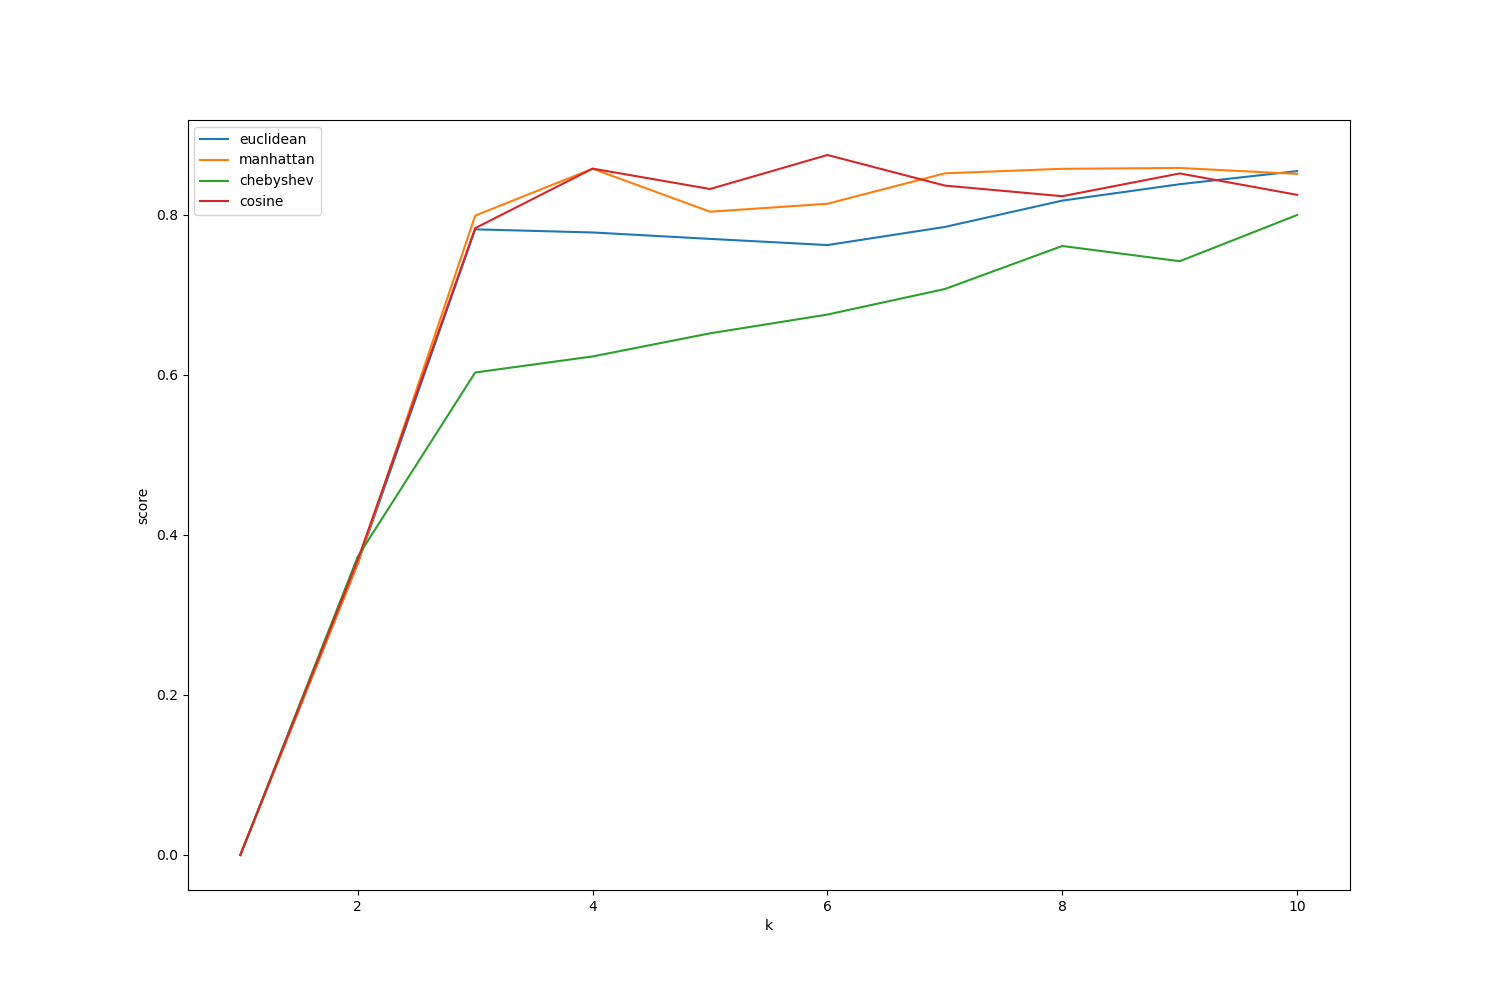
\includegraphics[width=0.45\textwidth]{../plots/wine/kmedoids/Homogeneity Score/k_1to10.png} }}%
	\qquad
	\subfloat[Silhouette Score ]{{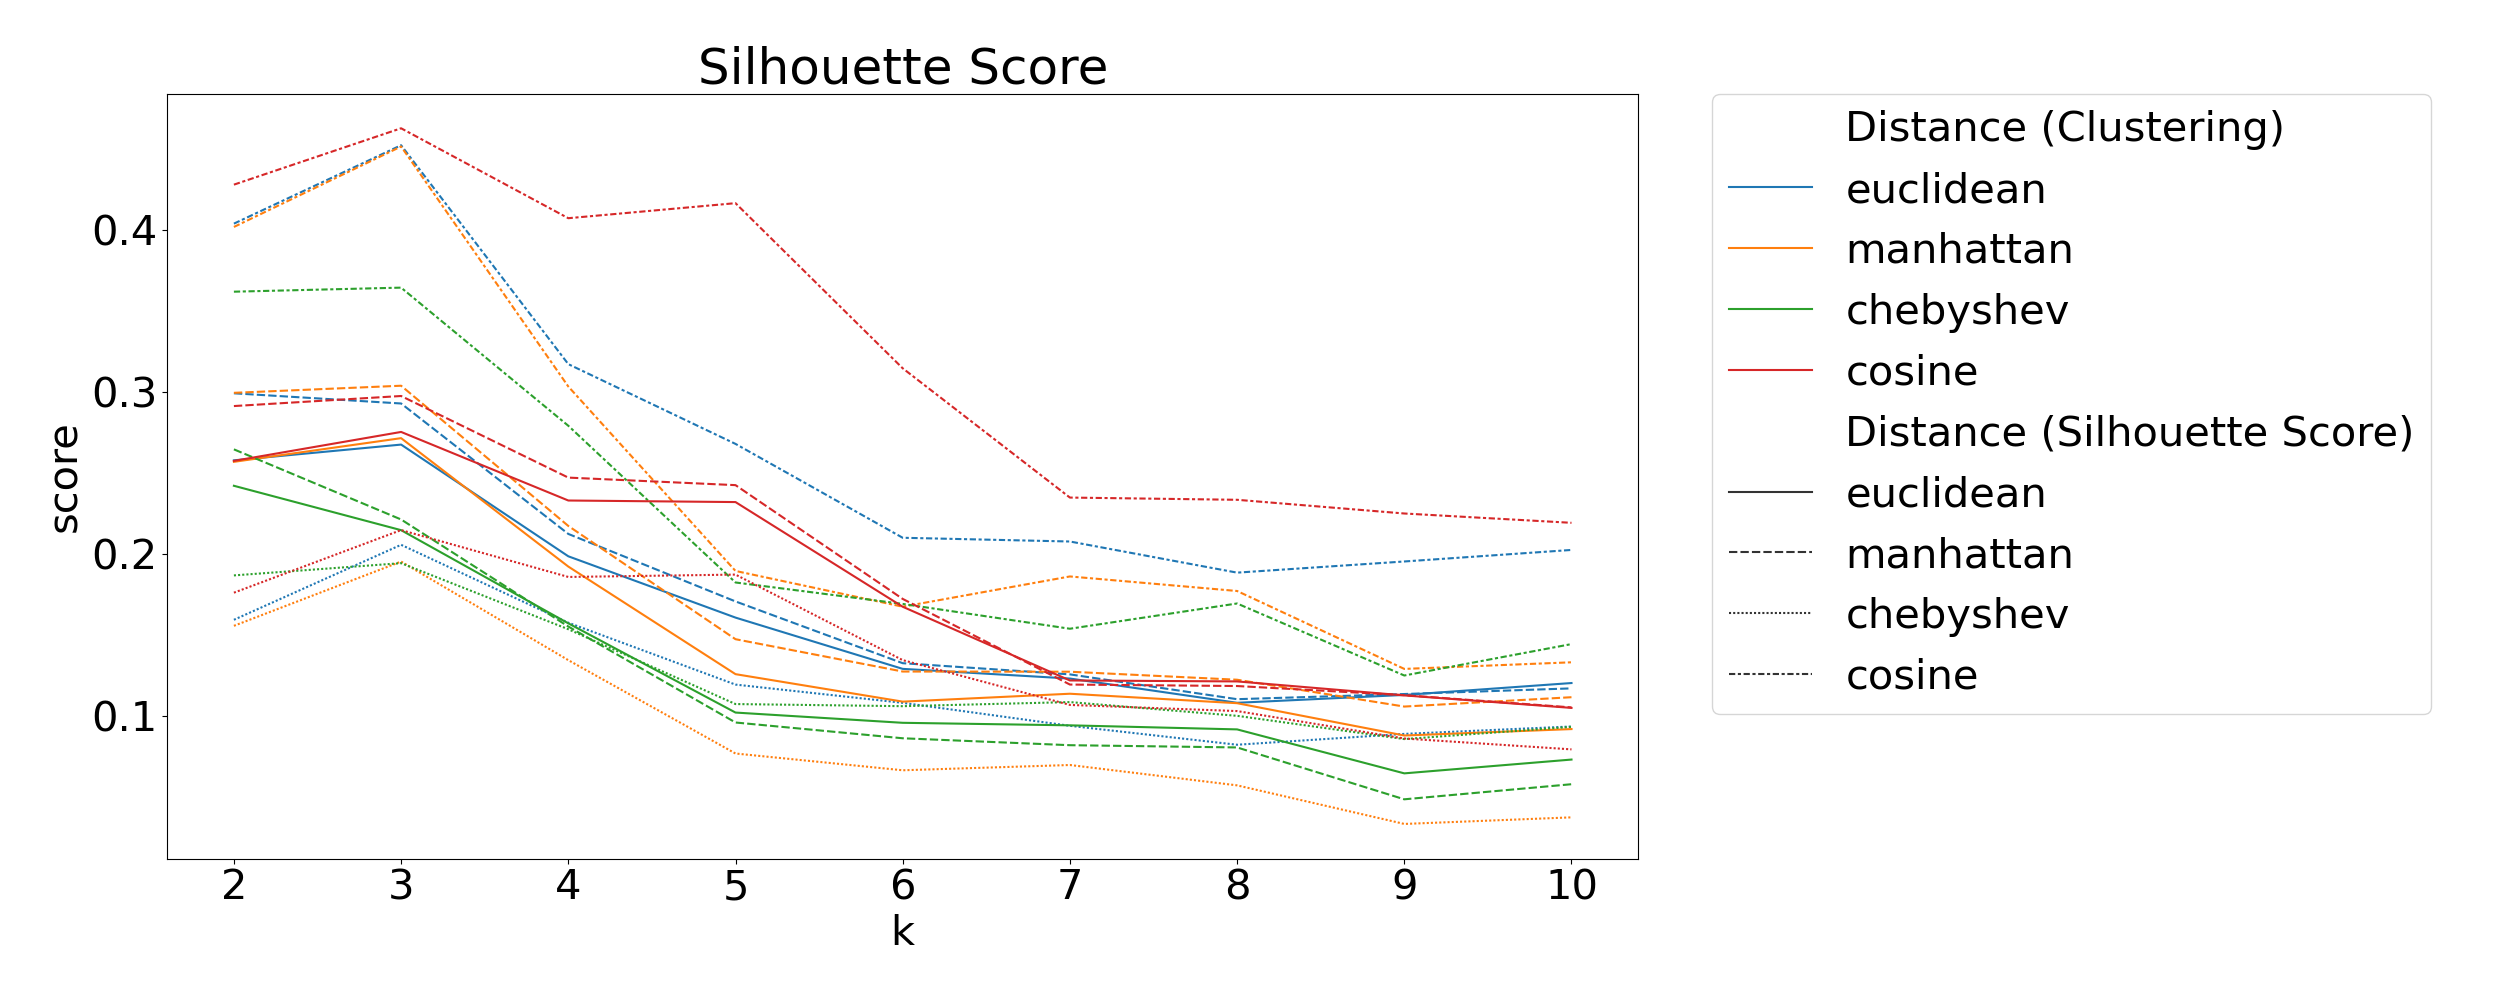
\includegraphics[width=1\textwidth]{../plots/wine/kmedoids/Silhouette Score/k_1to10.png} }}%
	
	\caption{Comparison of clustering scores for K-Medoids-clustering on Wine dataset}%
	\label{fig:kmedoids_wine}
\end{figure}

\begin{figure}[H]
	\centering
	\subfloat[Silhouette Score ]{{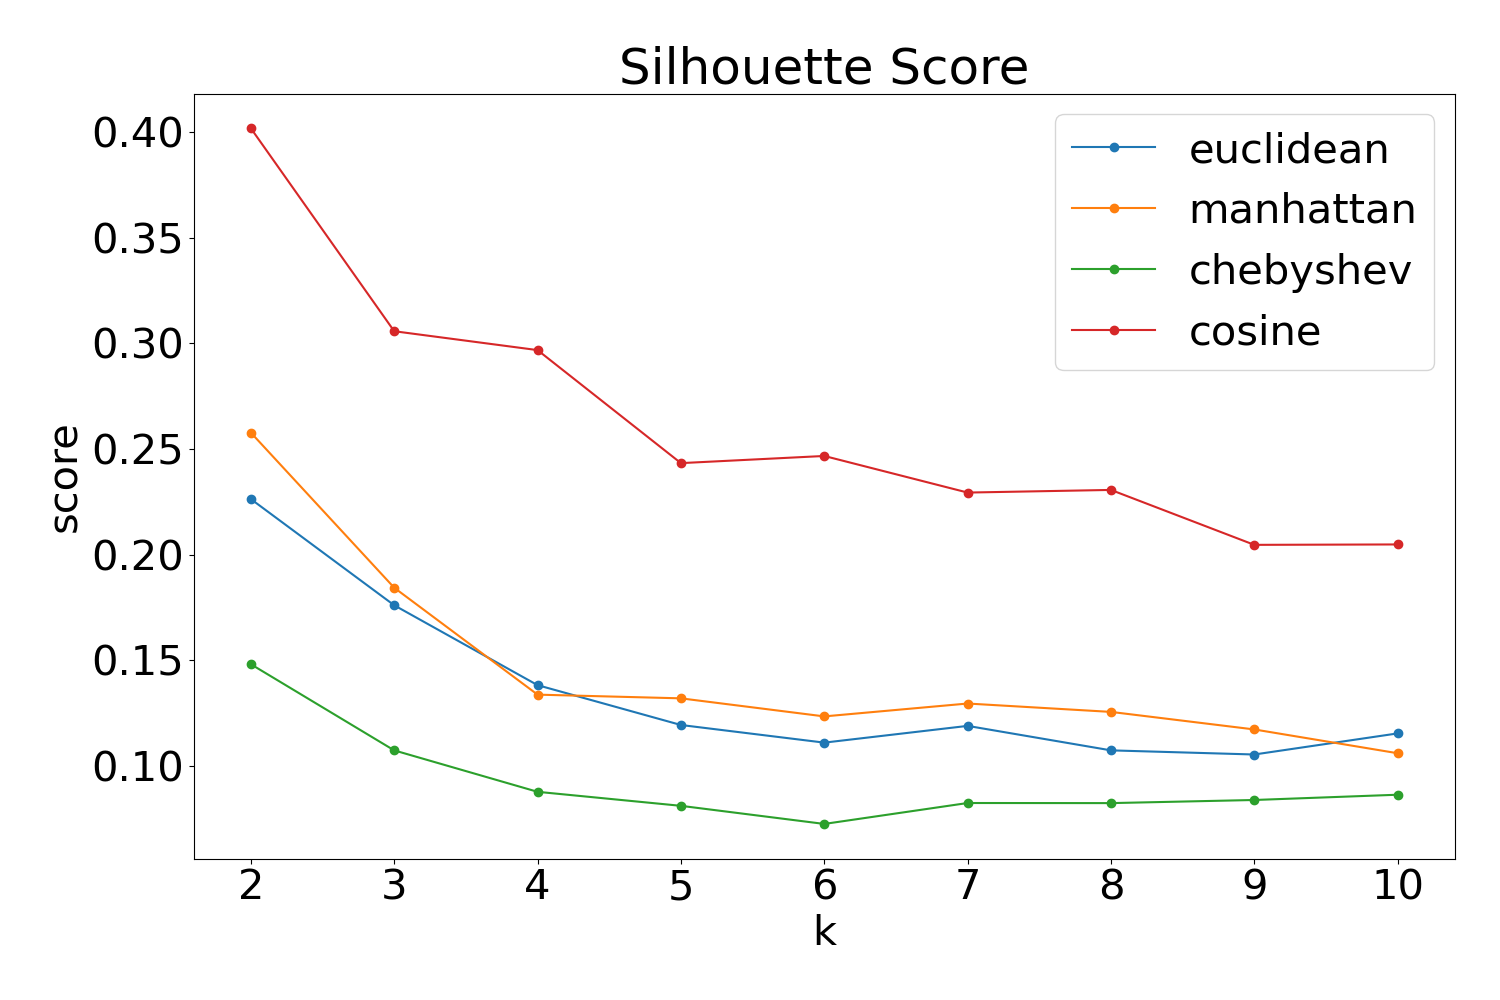
\includegraphics[width=1\textwidth]{../plots/diabetes/kmedoids/Silhouette Score/k_1to10.png} }}%
	
	\caption{Comparison of clustering scores for K-Medoids-clustering on Diabetes dataset}%
	\label{fig:kmedoids_diabetes}
\end{figure}

\begin{figure}[H]
	\centering
	\subfloat[ARI ]{{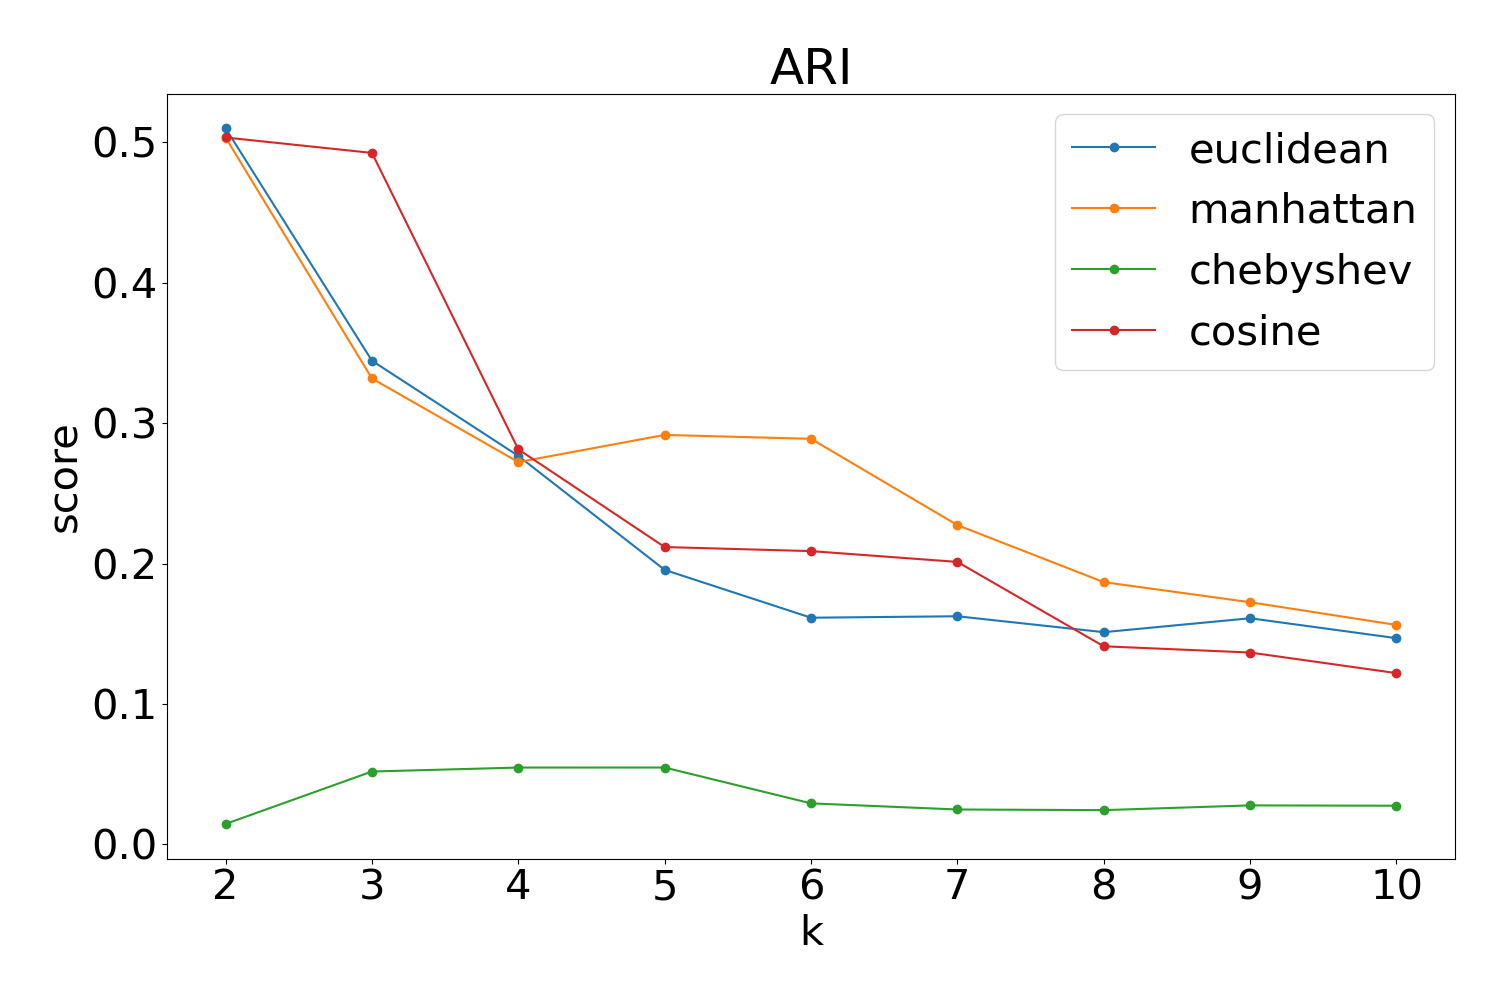
\includegraphics[width=0.45\textwidth]{../plots/housevotes/kmedoids/ARI/k_1to10.png} }}%
	\qquad
	\subfloat[AMI ]{{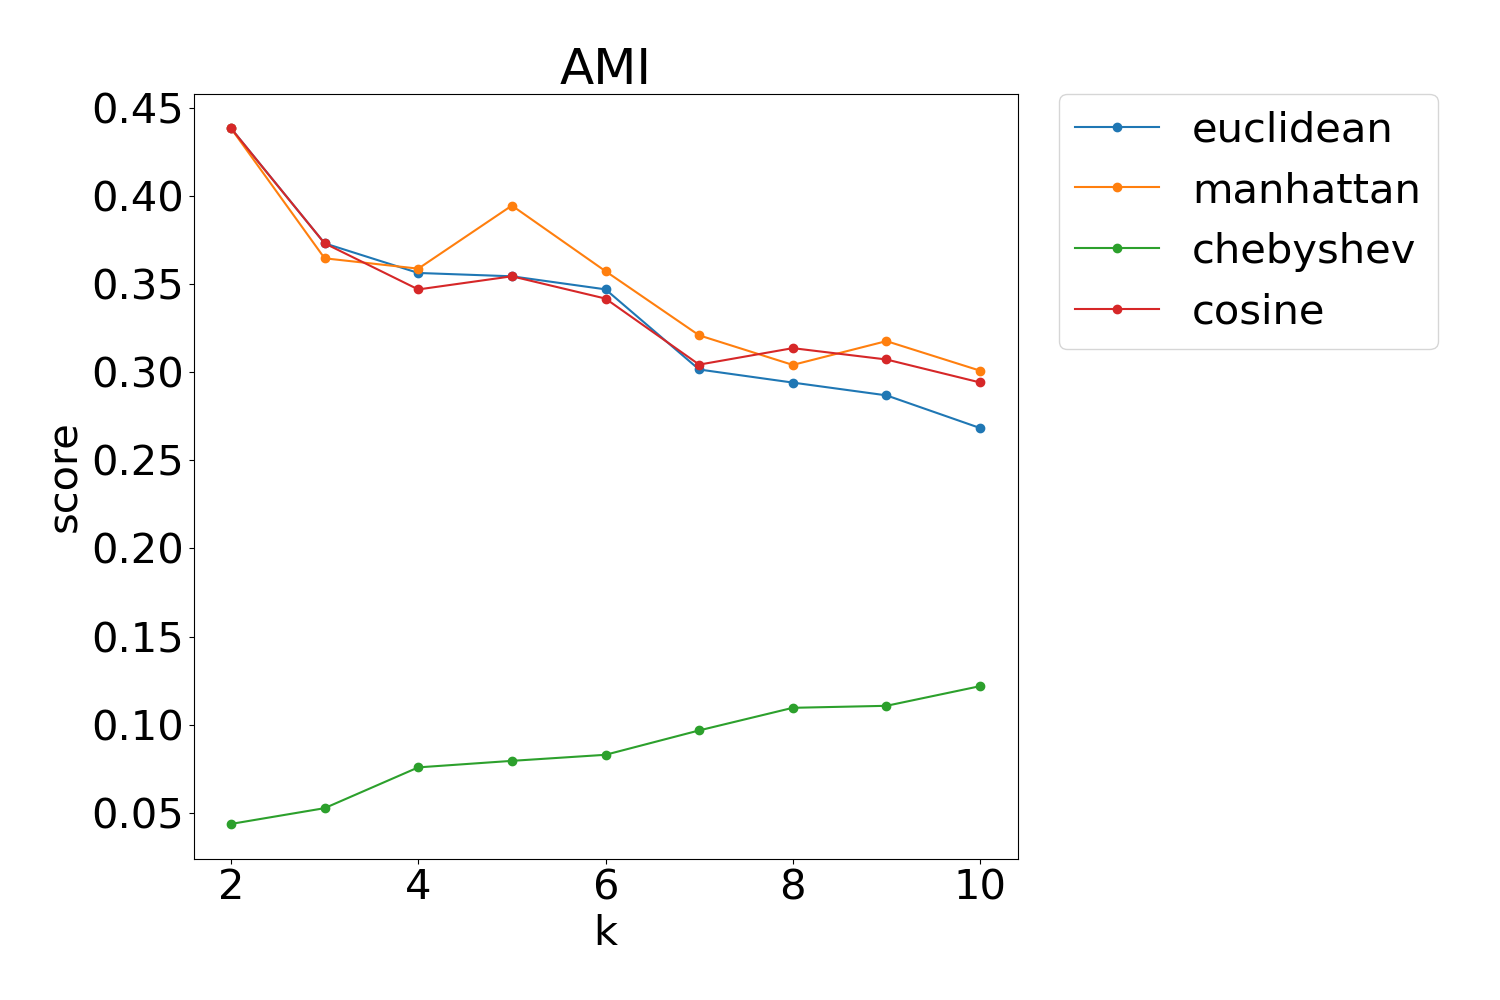
\includegraphics[width=0.45\textwidth]{../plots/housevotes/kmedoids/AMI/k_1to10.png} }}%
	\qquad
	\subfloat[Completeness Score ]{{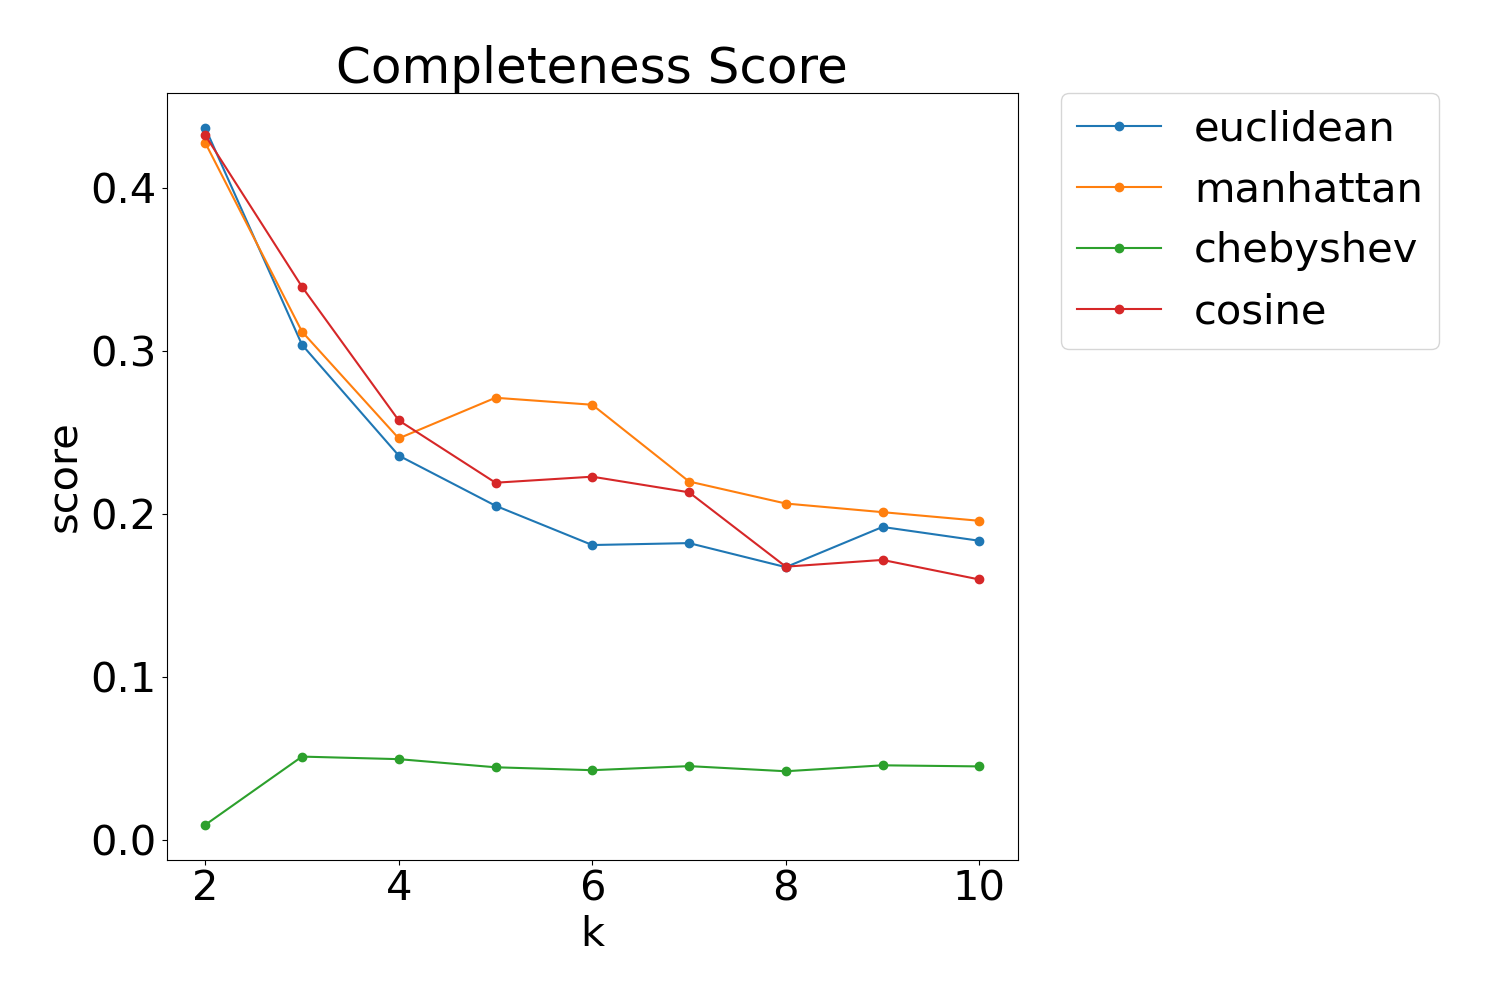
\includegraphics[width=0.45\textwidth]{../plots/housevotes/kmedoids/Completeness Score/k_1to10.png} }}%
	\qquad
	\subfloat[Homogeneity Score ]{{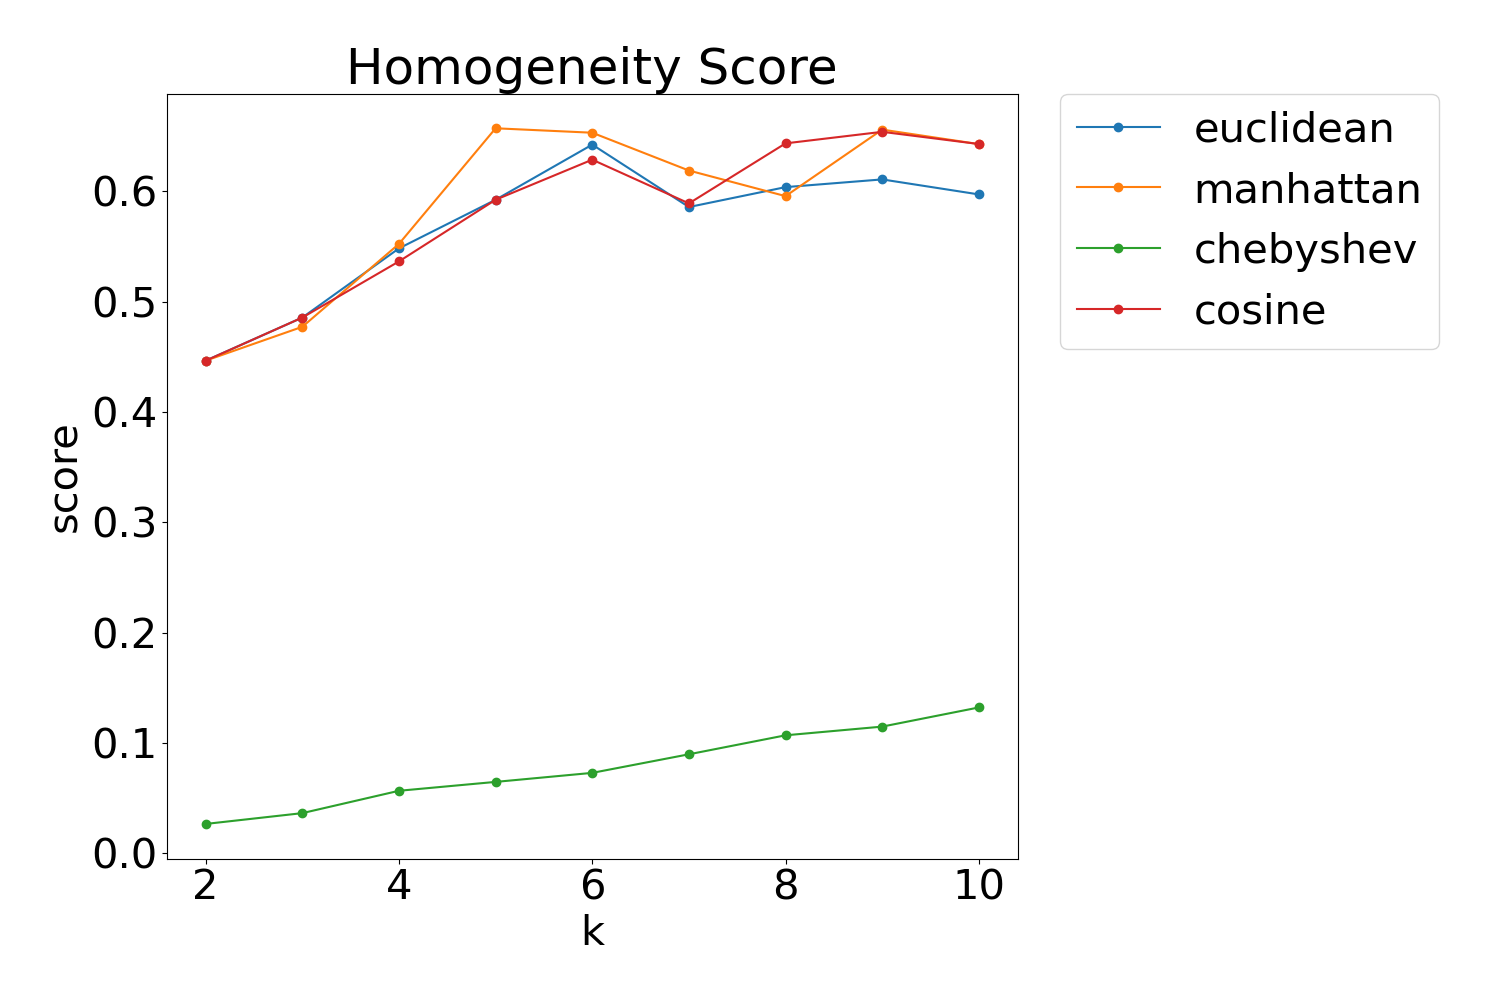
\includegraphics[width=0.45\textwidth]{../plots/housevotes/kmedoids/Homogeneity Score/k_1to10.png} }}%
	\qquad
	\subfloat[Silhouette Score ]{{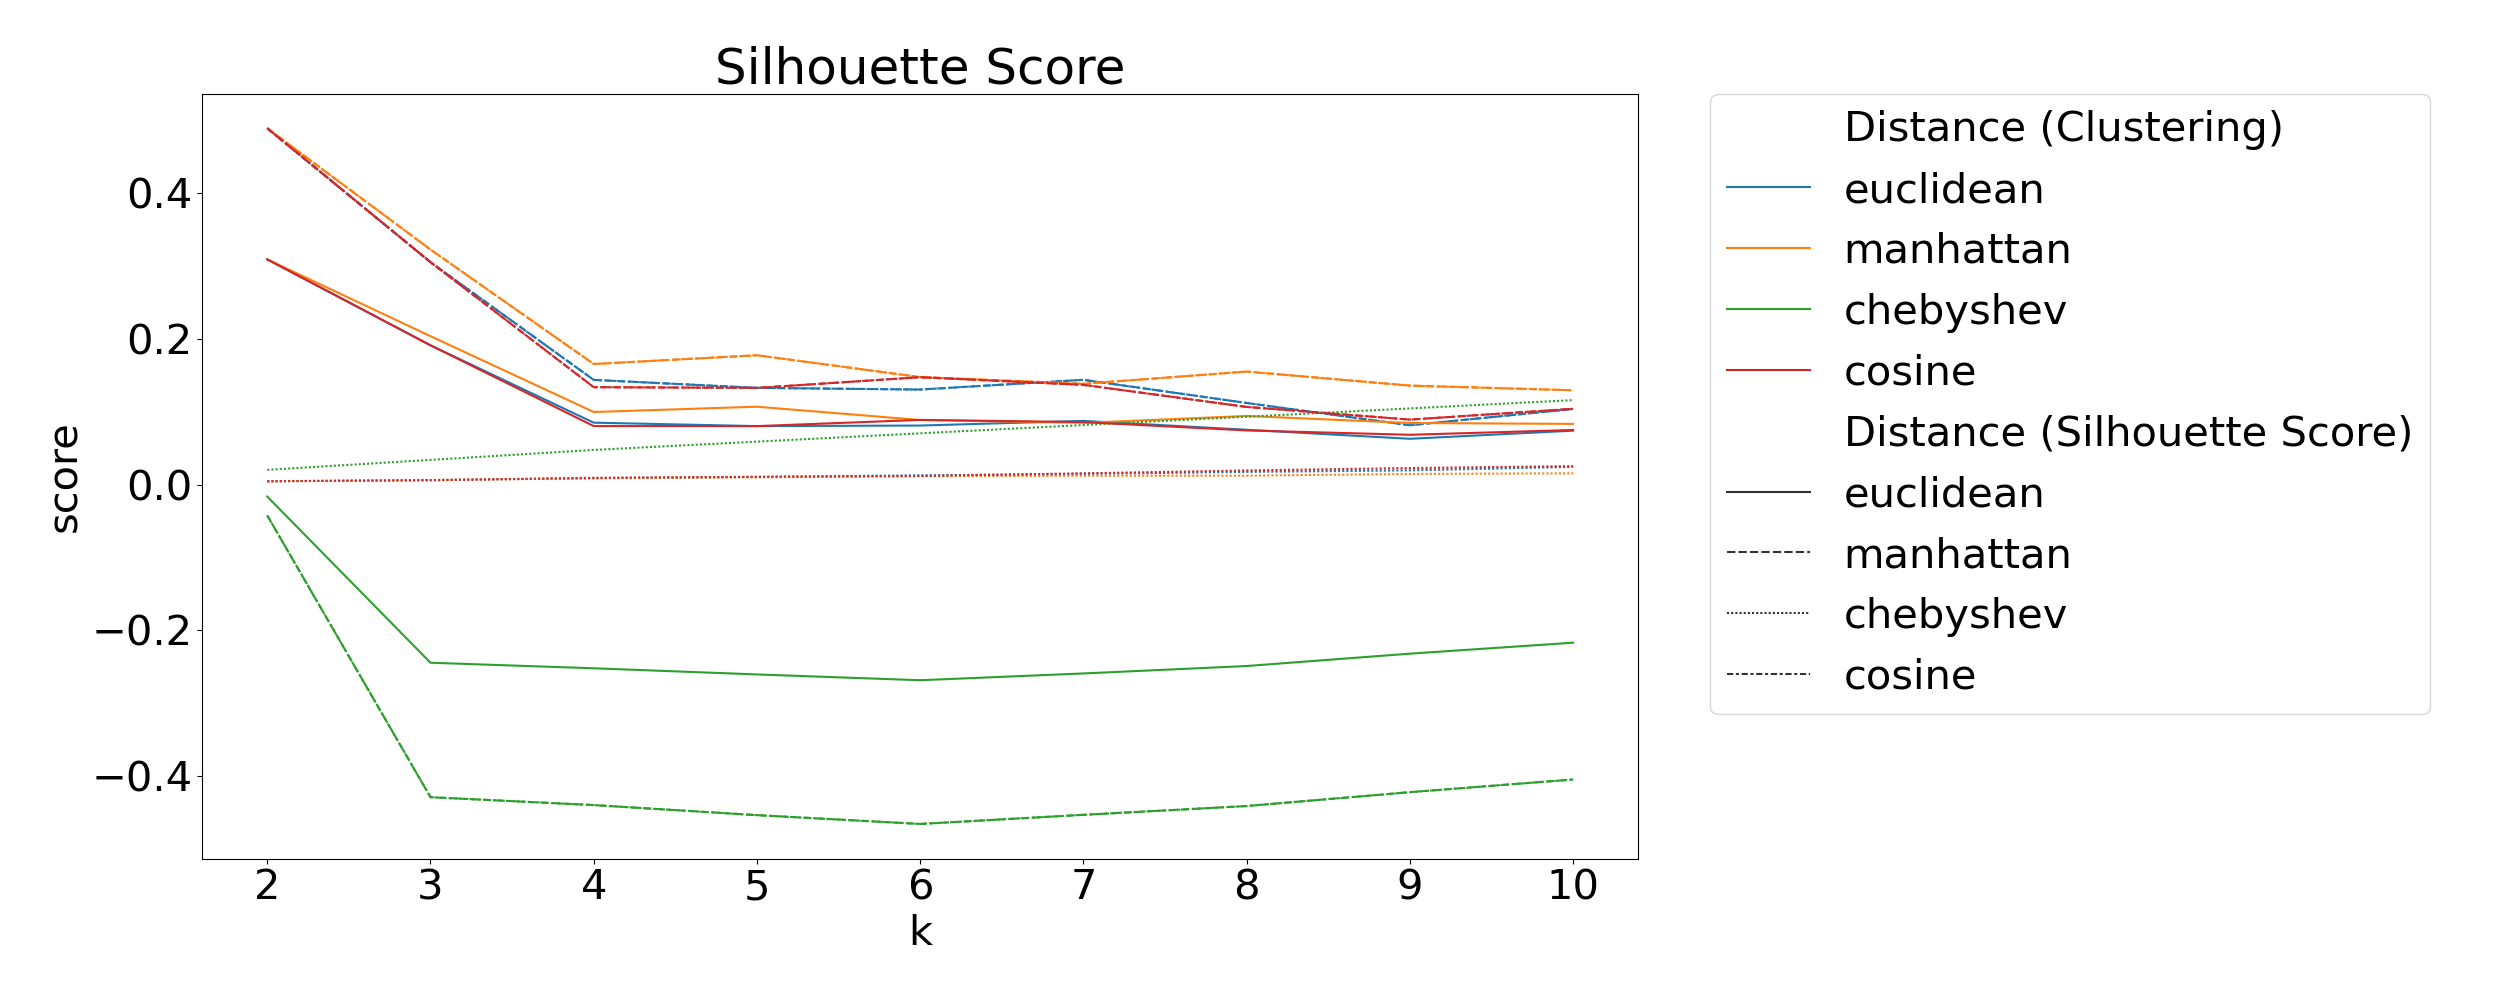
\includegraphics[width=1\textwidth]{../plots/housevotes/kmedoids/Silhouette Score/k_1to10.png} }}%
	
	\caption{Comparison of clustering scores for K-Medoids-clustering on Housevotes dataset}%
	\label{fig:kmedoids_housevotes}
\end{figure}



\subsection{Comparison for Given k Value}
For each dataset we independently compared clustering scores of different algorithms for multiple distances. For the algorithms that require a predefined number of clusters we set the value k to be the number of different classes in the dataset. For the diabetes dataset, which does not have categorical labels we have chosen k to be equal to the k value, that gives the highest Silhouette Score. \\
For the Silhouette Score the mean value and a standard deviation for the score evaluated with all four distance measures is shown. 

\begin{figure}[H]
	\centering
	\subfloat[ARI ]{{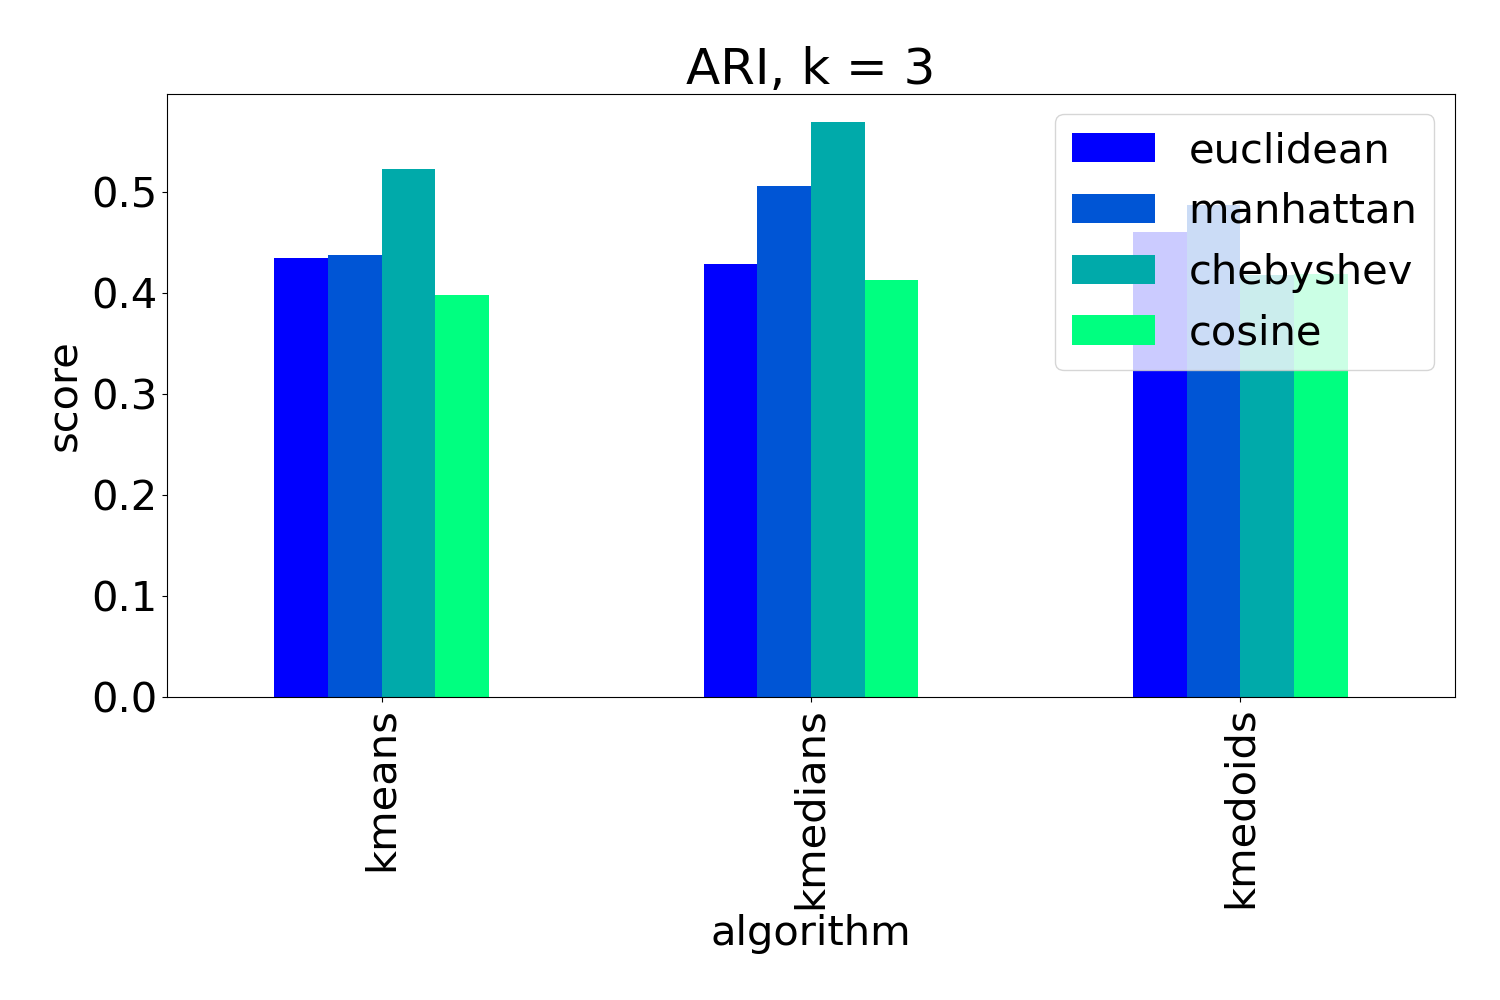
\includegraphics[width=0.45\textwidth]{../plots/iris/combined/ARI/algdist_for_given_k.png} }}%
	\qquad
	\subfloat[AMI ]{{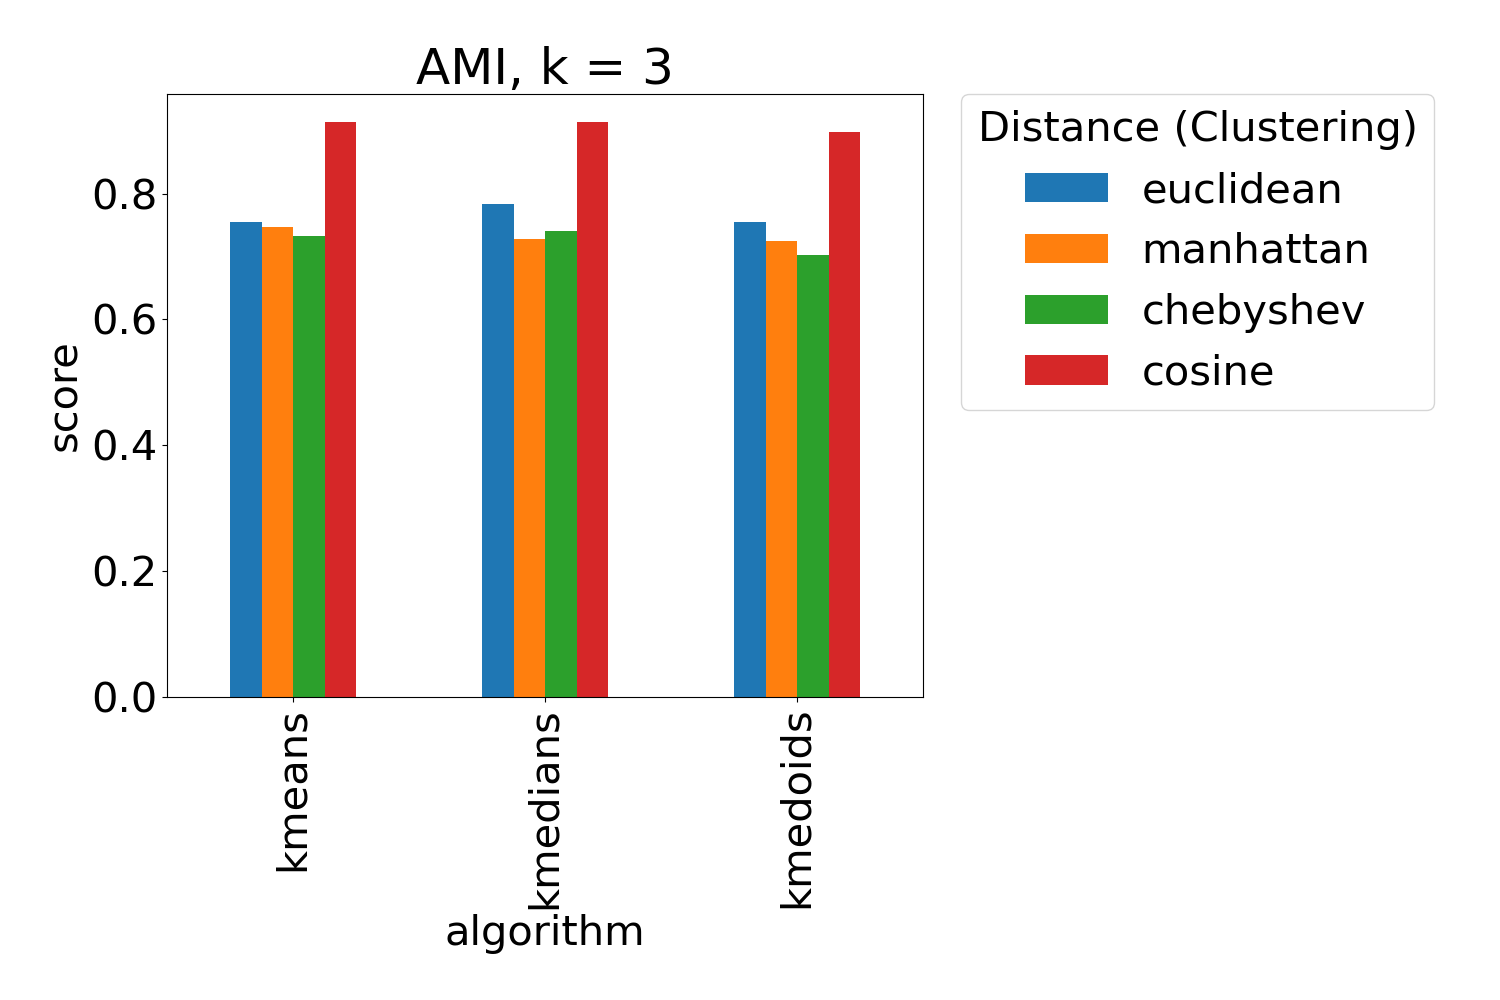
\includegraphics[width=0.45\textwidth]{../plots/iris/combined/AMI/algdist_for_given_k.png} }}%
	\qquad
	\subfloat[Completeness Score ]{{\includegraphics[width=0.45\textwidth]{../plots/iris/combined/Completeness Score/algdist_for_given_k.png} }}%
	\qquad
	\subfloat[Homogeneity Score ]{{\includegraphics[width=0.45\textwidth]{../plots/iris/combined/Homogeneity Score/algdist_for_given_k.png} }}%
	\qquad
	\subfloat[Silhouette Score ]{{\includegraphics[width=0.45\textwidth]{../plots/iris/combined/Silhouette Score/algdist_for_given_k.png} }}%
	
	\caption{Comparison of clustering scores for Iris dataset (given k=3)}%
	\label{fig:comparison_iris}
\end{figure}

\begin{figure}[H]
	\centering
	\subfloat[ARI ]{{\includegraphics[width=0.45\textwidth]{../plots/wine/combined/ARI/algdist_for_given_k.png} }}%
	\qquad
	\subfloat[AMI ]{{\includegraphics[width=0.45\textwidth]{../plots/wine/combined/AMI/algdist_for_given_k.png} }}%
	\qquad
	\subfloat[Completeness Score ]{{\includegraphics[width=0.45\textwidth]{../plots/wine/combined/Completeness Score/algdist_for_given_k.png} }}%
	\qquad
	\subfloat[Homogeneity Score ]{{\includegraphics[width=0.45\textwidth]{../plots/wine/combined/Homogeneity Score/algdist_for_given_k.png} }}%
	\qquad
	\subfloat[Silhouette Score ]{{\includegraphics[width=0.45\textwidth]{../plots/wine/combined/Silhouette Score/algdist_for_given_k.png} }}%
	
	\caption{Comparison of clustering scores for Wine dataset (given k=3)}%
	\label{fig:comparison_wine}
\end{figure}

\begin{figure}[H]
	\centering
	\subfloat[Silhouette Score ]{{\includegraphics[width=0.8\textwidth]{../plots/diabetes/combined/Silhouette Score/algdist_for_given_k.png} }}%
	
	\caption{Comparison of clustering scores for Diabetes dataset (given k=2)}%
	\label{fig:comparison_diabetes}
\end{figure}

\begin{figure}[H]
	\centering
	\subfloat[ARI ]{{\includegraphics[width=0.45\textwidth]{../plots/housevotes/combined/ARI/algdist_for_given_k.png} }}%
	\qquad
	\subfloat[AMI ]{{\includegraphics[width=0.45\textwidth]{../plots/housevotes/combined/AMI/algdist_for_given_k.png} }}%
	\qquad
	\subfloat[Completeness Score ]{{\includegraphics[width=0.45\textwidth]{../plots/housevotes/combined/Completeness Score/algdist_for_given_k.png} }}%
	\qquad
	\subfloat[Homogeneity Score ]{{\includegraphics[width=0.45\textwidth]{../plots/housevotes/combined/Homogeneity Score/algdist_for_given_k.png} }}%
	\qquad
	\subfloat[Silhouette Score ]{{\includegraphics[width=0.45\textwidth]{../plots/housevotes/combined/Silhouette Score/algdist_for_given_k.png} }}%
	
	\caption{Comparison of clustering scores for Housevotes dataset (given k=2)}%
	\label{fig:comparison_housevotes}
\end{figure}

\section{Comparison of Runtimes}
The runtimes were calculated on a custom build computer using a AMD Ryzen 3600X, 16GB 3200MHz DDR4 RAM. We took the average runtime of ten trials. The value k was set to be the number of different classes in the dataset for Iris, Wine and Housevotes dataset. For the Diabetes dataset, which does not have categorical labels we have chosen $k=2$ to be equal to the k value, that gives the highest Silhouette Score. For DBSCAN the parameters were used that give the highest ARI score for Iris, Wine and Housevotes and the highest Silhouette Score for Diabetes dataset. \\

\begin{table}[H]
	\begin{tabular}{lrrrr|r}
		\toprule
		{} &  Euclidean &  Manhattan &  Chebyshev &    Cosine &     Total \\
		\midrule
		K-Means   &   0.001300 &   0.001143 &   0.001214 &  0.057548 &  0.061206 \\
		K-Medians &   0.001824 &   0.002235 &   0.005253 &  0.873826 &  0.883138 \\
		K-Medoids &   0.032768 &   0.026929 &   0.030192 &  0.269327 &  0.359216 \\
		DBSCAN    &   0.000683 &   0.000736 &   0.000640 &  0.000805 &  0.002864 \\
		\midrule
		Total     &   0.036575 &   0.031044 &   0.037299 &  1.201506 &  1.306424 \\
		\bottomrule
		
	\end{tabular}
	\caption{Runtimes for Iris dataset (in seconds)}
\end{table}


\begin{table}[H]
	\begin{tabular}{lrrrr|r}
		\toprule
		{} &  Euclidean &  Manhattan &  Chebyshev &    Cosine &     Total \\
		\midrule
		K-Means   &   0.001686 &   0.001692 &   0.001632 &  0.112143 &  0.117153 \\
		K-Medians &   0.003722 &   0.004837 &   0.005135 &  0.074670 &  0.088364 \\
		K-Medoids &   0.112080 &   0.091926 &   0.102531 &  0.462057 &  0.768594 \\
		DBSCAN    &   0.001123 &   0.001168 &   0.000848 &  0.000895 &  0.004034 \\
		\midrule
		Total     &   0.118611 &   0.099622 &   0.110146 &  0.649764 &  0.978144 \\
		\bottomrule
		
	\end{tabular} 
	\caption{Runtimes for Wine dataset (in seconds)}
\end{table}


\begin{table}[H]
	\begin{tabular}{lrrrr|r}
		\toprule
		{} &  Euclidean &  Manhattan &  Chebyshev &    Cosine &     Total \\
		\midrule
		K-Means   &   0.005803 &   0.003188 &   0.003208 &  0.136975 &  0.149174 \\
		K-Medians &   0.012511 &   0.014224 &   0.014343 &  0.134298 &  0.175376 \\
		K-Medoids &   0.558538 &   0.455667 &   0.481983 &  2.495598 &  3.991786 \\
		DBSCAN    &   0.003577 &   0.004333 &   0.003563 &  0.002348 &  0.013822 \\
		\midrule
		Total     &   0.580429 &   0.477412 &   0.503097 &  2.769219 &  4.330157 \\
		\bottomrule
		
	\end{tabular}
	\caption{Runtimes for Diabetes dataset (in seconds)}
\end{table}


\begin{table}[H]
	\begin{tabular}{lrrrr|r}
		\toprule
		{} &  Euclidean &  Manhattan &  Chebyshev &    Cosine &      Total \\
		\midrule
		K-Means   &   0.005589 &   0.005560 &   0.008237 &  0.341636 &   0.361021 \\
		K-Medians &   0.281766 &   0.285803 &   0.011203 &  0.220306 &   0.799078 \\
		K-Medoids &   2.093371 &   1.815214 &   1.911084 &  6.242655 &  12.062324 \\
		DBSCAN    &   0.011879 &   0.012103 &   0.006456 &  0.004406 &   0.034844 \\
		\midrule
		Total     &   2.392605 &   2.118680 &   1.936980 &  6.809003 &  13.257267 \\
		\bottomrule
	\end{tabular}
	\caption{Runtimes for Housevotes dataset (in seconds)}
\end{table}

